\documentclass[fr]{../../../eplexercises}

\RequirePackage{titlesec}
\titleformat
{\section} % command
[hang] % shape
{\bfseries\Large} % format
{\thesection} % label
{0.5ex} % sep
{} % before-code

\usepackage{../fitch}
\usepackage{pdfpages}

\usepackage{../../../eplcode}
\definecolor{mygray}{rgb}{0.5,0.5,0.5} % needed by: 14, 17
\lstset{language=Prolog, frame = single, numbers=left, numbersep=-0.5cm, numberstyle=\small\color{mygray}, escapeinside={\%*}{*)}}

\newcommand{\true}{\mathrm{true}}
\newcommand{\false}{\mathrm{false}}
\newcommand{\val}{\mathrm{val}}
\newcommand{\VAL}{\mathrm{VAL}}
\newcommand{\decale}{\par\nodecale\hspace*{20pt}\ignorespaces}

\hypertitle{logique-INGI1101}{5}{INGI}{1101}
{Maxime Dimidschstein\and Basile Cassiers\and Nicolas Vanvyve\and Adrien Ballet\and Samuel Monroe\and Sébastien Mottet\and Grâce Musuvaho\and  Mathias Novak\and Céline Deknop}
{Peter Van Roy}

% OR
\pgfkeys{
	orGate/.is family,
	orGate,
	x/.initial=0,
	y/.initial=0,
	l/.initial=or,
}
\newcommand\orGateSet[1]{\pgfkeys{orGate, #1}}
\newcommand\orGate[1][]{
	\orGateSet{#1,
    x/.get=\x,
    y/.get=\y,
		l/.get=\l,
  }
	\draw (\x, 1 + \y) to [out=0,in=120] (0.85 + \x, 0.5 + \y);
	\draw (\x, \y) to [out=0,in=250] (0.85 + \x, 0.5 + \y);
	\draw (\x, \y) to [out=60,in=270] (0.2 + \x, 0.5 + \y);
	\draw (\x, 1 + \y) to [out=300,in=90] (0.2 + \x, 0.5 + \y);
	\draw (\x, 0.2 + \y) -- (0.12 + \x, 0.2 + \y);
	\draw (\x, 0.8 + \y) -- (0.12 + \x, 0.8 + \y);
	\draw (0.85 + \x, 0.5 + \y) -- (1 + \x, 0.5 + \y);
	\node at (\x + 0.5, \y + 0.5) {\tiny \textsf{\l}};
}

% NOR
\pgfkeys{
	norGate/.is family,
	norGate,
	x/.initial=0,
	y/.initial=0,
	l/.initial=nor,
}
\newcommand\norGateSet[1]{\pgfkeys{norGate, #1}}
\newcommand\norGate[1][]{
	\norGateSet{#1,
    x/.get=\x,
    y/.get=\y,
		l/.get=\l,
  }
	\draw (\x, 1 + \y) to [out=0,in=120] (0.85 + \x, 0.5 + \y);
	\draw (\x, \y) to [out=0,in=250] (0.85 + \x, 0.5 + \y);
	\draw (\x, \y) to [out=60,in=270] (0.2 + \x, 0.5 + \y);
	\draw (\x, 1 + \y) to [out=300,in=90] (0.2 + \x, 0.5 + \y);
	\draw (\x, 0.2 + \y) -- (0.12 + \x, 0.2 + \y);
	\draw (\x, 0.8 + \y) -- (0.12 + \x, 0.8 + \y);
	\draw (0.85 + \x, 0.5 + \y) -- (1 + \x, 0.5 + \y);
	\draw[fill = white] (0.85 + \x, 0.5 + \y) circle (0.04);
	\node at (\x + 0.5, \y + 0.5) {\tiny \textsf{\l}};
}

% AND
\pgfkeys{
	andGate/.is family,
	andGate,
	x/.initial=0,
	y/.initial=0,
	l/.initial=and,
}
\newcommand\andGateSet[1]{\pgfkeys{andGate, #1}}
\newcommand\andGate[1][]{
	\andGateSet{#1,
    x/.get=\x,
    y/.get=\y,
		l/.get=\l,
  }
	\draw (0.1 + \x, \y) -- (0.1 + \x, 1 + \y);
	\draw (0.1 + \x, \y) -- (0.6 + \x, \y);
	\draw (0.1 + \x, 1 + \y) -- (0.6 + \x, 1 + \y);
	\draw (0.6 + \x, \y) to [out=0, in=270] (0.9 + \x, 0.5 + \y);
	\draw (0.6 + \x, 1 + \y) to [out=0, in=90] (0.9 + \x, 0.5 + \y);
	\draw (\x, 0.2 + \y) -- (0.1 + \x, 0.2 + \y);
	\draw (\x, 0.8 + \y) -- (0.1 + \x, 0.8 + \y);
	\draw (0.9 + \x, 0.5 + \y) -- (1 + \x, 0.5 + \y);
	\node at (\x + 0.5, \y + 0.5) {\tiny \textsf{\l}};
}

% NAND
\pgfkeys{
	nandGate/.is family,
	nandGate,
	x/.initial=0,
	y/.initial=0,
	l/.initial=nand,
}
\newcommand\nandGateSet[1]{\pgfkeys{nandGate, #1}}
\newcommand\nandGate[1][]{
	\nandGateSet{#1,
    x/.get=\x,
    y/.get=\y,
		l/.get=\l,
  }
	\draw (0.1 + \x, \y) -- (0.1 + \x, 1 + \y);
	\draw (0.1 + \x, \y) -- (0.6 + \x, \y);
	\draw (0.1 + \x, 1 + \y) -- (0.6 + \x, 1 + \y);
	\draw (0.6 + \x, \y) to [out=0, in=270] (0.9 + \x, 0.5 + \y);
	\draw (0.6 + \x, 1 + \y) to [out=0, in=90] (0.9 + \x, 0.5 + \y);
	\draw (\x, 0.2 + \y) -- (0.1 + \x, 0.2 + \y);
	\draw (\x, 0.8 + \y) -- (0.1 + \x, 0.8 + \y);
	\draw (0.9 + \x, 0.5 + \y) -- (1 + \x, 0.5 + \y);
	\draw[fill = white] (0.9 + \x, 0.5 + \y) circle (0.04);
	\node at (\x + 0.5, \y + 0.5) {\tiny \textsf{\l}};
}

% NOT
\pgfkeys{
	notGate/.is family,
	notGate,
	x/.initial=0,
	y/.initial=0,
	l/.initial=not,
}
\newcommand\notGateSet[1]{\pgfkeys{notGate, #1}}
\newcommand\notGate[1][]{
	\notGateSet{#1,
    x/.get=\x,
    y/.get=\y,
		l/.get=\l,
  }
	\draw (0.1 + \x, \y) -- (0.1 + \x, 1 + \y);
	\draw (0.1 + \x, \y) -- (0.9 + \x, 0.5 + \y);
	\draw (0.1 + \x, 1 + \y) -- (0.9 + \x, 0.5 + \y);
	\draw (\x, 0.5 + \y) -- (0.1 + \x, 0.5 + \y);
	\draw (0.9 + \x, 0.5 + \y) -- (1 + \x, 0.5 + \y);
	\draw[fill = white] (0.9 + \x, 0.5 + \y) circle (0.04);
	\node at (\x + 0.4, \y + 0.5) {\tiny \textsf{\l}};
}

% T
\pgfkeys{
	tWire/.is family,
	tWire,
	x/.initial=0,
	y/.initial=0,
}
\newcommand\tWireSet[1]{\pgfkeys{tWire, #1}}
\newcommand\tWire[1][]{
	\notGateSet{#1,
    x/.get=\x,
    y/.get=\y,
  }
	\draw (\x, 0.5 + \y) -- (\x + 1, 0.5 + \y);
	\draw (\x + 0.5, 0.5 + \y) -- (\x + 0.5 , \y);
}

\pgfkeys{
  mygrid/.is family,
  mygrid,
  min x/.initial=-5,
  max x/.initial=5,
  min y/.initial=-5,
  max y/.initial=5,
  small step/.initial=.1,
  step/.initial=1,
  big step/.initial=5,
  color/.initial=red,
}
\newcommand\mygridset[1]{\pgfkeys{mygrid,#1}}
\newcommand\mygrid[1][]{
  \mygridset{#1,
    min x/.get=\gridminx,
    max x/.get=\gridmaxx,
    min y/.get=\gridminy,
    max y/.get=\gridmaxy,
    small step/.get=\gridsmallstep,
    step/.get=\gridstep,
    big step/.get=\gridbigstep,
    color/.get=\gridcolor
  }

  \draw [step=\gridsmallstep, help lines,\gridcolor!20]
  (\gridminx,\gridminy) grid (\gridmaxx,\gridmaxy);
  \draw [step=\gridstep, help lines,\gridcolor!40]
  (\gridminx,\gridminy) grid (\gridmaxx,\gridmaxy);
  \draw [step=\gridbigstep, help lines,\gridcolor!100]
  (\gridminx,\gridminy) grid (\gridmaxx,\gridmaxy);
  \foreach \x in {\gridminx,...,\gridmaxx} {
    \node[below,font=\tiny] at (\x,\gridminy) {$\x$};
    \node[above,font=\tiny] at (\x,\gridmaxy) {$\x$};
  };
  \foreach \y in {\gridminy,...,\gridmaxy} {
    \node[left,font=\tiny] at (\gridminx,\y) {$\y$};
    \node[right,font=\tiny] at (\gridmaxx,\y) {$\y$};
  };
}

\newcommand\loeq{\Lleftarrow\!\!\!\!\Rrightarrow }

\newcommand\enter[0]{
	{\color{white} newline}
}

\newif\ifanswers
\answerstrue

\newenvironment{sol}
{
\textbf{Solution} \\
}
{
\vspace{0.25cm}
}
\renewcommand\t[1]{\text{#1}}


\section*{À propos}
Ce document reprend les solutions des exercices du cours LINGI1101 dispensé par M. Peter Van Roy au cours de l'année académique 2016-2017.\\
La quasi totalité de ces solutions ont été rédigées par des étudiants, et il est donc important de rester critique en les consultant : des erreurs subsistent, et la matière peut avoir changé.

Une partie du document a été révisée par un assistant, François Aubry, et cette correction datant de janvier 2017 se trouve \href{https://github.com/Gp2mv3/Syntheses/tree/master/src/q5/logique-INGI1101/exercises/Other}{ici}.

\vspace{2ex}
N'hésitez pas à vous servir de ce document et à le reprendre pour le corriger, l'améliorer et l'étendre.

\paragraph{\large{N.B. :}} Bien que les TP portent en grande partie sur les preuves, l'examen est lui beaucoup plus théorique et porte sur des exemples vu au cours.
%\section*{TEMPLATE}
Le syllabus peut être trouvé à l'adresse \url{https://github.com/petervanroy/lingi1101}.
C'est de là que proviennent la majorité des templates utilisés dans ce solutionnaire, inspirez-vous en.\\
Lorsque vous trouvez une nouvelle structure qui n'a pas encore été employée dans ce rapport, tapez-en un exemple ici dans une section, en plus de la mettre dans votre partie.
(Et faites en sorte que ça compile!)
Comme ça les prochains pourront également s'en servir sans devoir fouiller partout.\\
Cette partie ne sera pas inclue dans le rapport final, elle sert uniquement lors de sa rédaction.

\subsection*{Quantificateurs et symboles}
\begin{itemize}
    \item \textbf{Et logique} : $\land$
    \item \textbf{Ou logique} : $\lor$
    \item \textbf{Négation} : $\neg$
    \item \textbf{Pour tout} : $\forall$
    \item \textbf{Il existe} : $\exists$
    \item \textbf{Implication} : $\Rightarrow$
    \item \textbf{Si et seulement si} : $\Leftrightarrow$
    \item \textbf{Tautologie} : $\models$
    \item \textbf{Conséquence logique} : $\Rrightarrow$
    \item \textbf{Équivalence logique} : $\Lleftarrow \Rrightarrow$
\end{itemize}


\subsection*{Règle - cas - résultat}
\begin{enumerate}
  \item Règle: $\forall$ $x$, $sac(x)$ $\Rightarrow$ $blanc(x)$
  \item Cas: $sac(a)$, $sac(b)$, $\cdots$\\
  \rule{5.5cm}{.1pt} 
  \item Résultat: $blanc(a)$, $blanc(b)$, $\cdots$
\end{enumerate}

\subsection*{Table de vérité}
\begin{center}
	\begin{tabular}{cc|ccccc}
		$P$ & $Q$ & $\lnot P$ & $\lnot Q$ & $\lnot( P \land Q)$ & $P \land Q$ & $ (\lnot P \lor \lnot Q)$\\
		\hline
		F&F&T&T&T&F&T\\
		T&F&F&T&T&F&T\\
		F&T&T&F&T&F&T\\
		T&T&F&F&F&T&F\\
	\end{tabular}
\end{center}

\subsection*{Règle BNF}
\begin{tabular}{rrl}
  $\textrm{<identificateur>}$ & ::= & $A$ | $B$ | $C$ | $D$ | \dots \\
  $\textrm{<proposition>}$
  & ::= & $\true$ \\
  & | & $\false$ \\
  & | & $\textrm{<identificateur>}$ \\
  & | & $(\textrm{<proposition>})$ \\
  & | & $\lnot \textrm{<proposition>}$ \\
  & | & $\textrm{<proposition>} \land \textrm{<proposition>}$ \\
  & | & $\textrm{<proposition>} \lor \textrm{<proposition>}$ \\
  & | & $\textrm{<proposition>} \Rightarrow \textrm{<proposition>}$ \\
  & | & $\textrm{<proposition>} \Leftrightarrow \textrm{<proposition>}$
\end{tabular}

%\subsection*{Pseudocode}

%\begin{algorithm}[H]
%\While{$false \not\in S$ et $\exists$? clauses résolvables non résolues}{
%	\begin{itemize}
%		\item choisir $C_1,C_2 \in S$ tel que $\exists P \in C_1, \lnot P \in C_2$ 		
%		\item calculer r:=$C_1 - \{P\} \lor C_2 - \{\lnot P\}$
%		\item calculer S:= $S \cup \{r\}$
%	\end{itemize}
%}
%\eIf{$false \in S$}{C est prouvé}{C n'est pas prouvé}
%\end{algorithm}

\subsubsection*{Exemple de résolution}
\begin{tabbing}
\hspace{3cm}\=\hspace{2cm}\=\kill
C$_{1}$ : P $\lor$ Q \\
C$_{2}$ : P $\lor$ R \\
C$_{3}$ : $\lnot$Q $\lor$ $\lnot$R \\
C : P \> \> \{C$_{1}$,C$_{2}$,C$_{3}$,$\lnot$C\}
\end{tabbing}

\noindent \emph{Quelques pas de résolution :}

\noindent C$_{1}$ + $\lnot$C $\rightarrow$  Q (C$_{5}$) \newline
C$_{2}$ + $\lnot$C $\rightarrow$ R  (C$_{6}$) \newline
C$_{3}$ + C$_{5}$ $\rightarrow$ $\lnot$R (C$_{7}$) \newline 
C$_{6}$ + C$_{7}$ $\rightarrow$ \underline{false} ($\in$ S donc C est prouvé) \newline


\subsubsection*{Preuve}

\begin{tabular}{|l|l|}
\hline
1. A$\Rightarrow$B & prémisse \\
2. C$\Rightarrow$D & prémisse \\
3. B$\lor$D $\Rightarrow$E & prémisse \\
4. $\lnot$E & prémisse \\ 
\indent 5. A & hypothèse \\
\indent 6. B & modus ponens (1) \\
\indent 7. B$\lor$D & addition (6) \\
\indent 8. E & modus ponens (7) \\
9. $\lnot$A & preuve indirecte \\
\indent 10. C & hypothèse \\
\indent 11. D & modus ponens (2) \\
\indent 12. D$\lor$B & addition (11) \\
\indent 13. B$\lor$D & commutativité (12)\\
\indent 14. E & modus ponens (9) \\
15. $\lnot$C & preuve indirecte \\
16. $\lnot$A $\land$ $\lnot$C & conjonction (9,15) \\
\hline
\end{tabular}\\

\subsection*{Tracer des graphes avec Tikz}

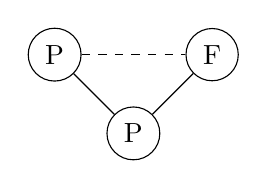
\begin{tikzpicture}
\coordinate (A) at (0,1);
\coordinate (B) at (1,0);
\coordinate (C) at (2,1);


\node[draw,circle] (A) at (A){P};
\node[draw,circle] (B) at (B){P};
\node[draw] (C) at (C){F};

\draw  (A)--(B);
\draw [dashed] (A)--(C);
\draw (C)--(B);

\end{tikzpicture}



\section{}
\subsection{Exercise 1 (Perfect secrecy.)}
We define the following encryption scheme for messages, keys and
ciphertexts in $\mathbb{Z}_n$, where $\mathbb{Z}_n$ is essentially 
the integers in the interval $[0,n[$ 
(in fact $(\mathbb{Z}_n,+)$ forms a group):
\smallskip
\begin{itemize}
  \item $\Gen$ outputs a key $k \in \K$ selected uniformly at random.
  \item $\Enc_k(m) := k+m \mod n$
  \item $\Dec_k(c) := c-k \mod n$
\end{itemize}
\smallskip
Suppose messages are drawn from $\M$ according to the binomial
distribution. More precisely $M\sim \mathrm{Bi}(n-1,p)$ for some probability $p$ 
which means that $\forall m\in \M: \Pr[M=m]=\binom{n-1}{m}p^{m}(1-p)^{n-1-m}$.
\smallskip
\begin{enumerate}
  \item Show that the encryption scheme above is perfectly secret.
  \item Evaluate $\Pr[C=c]$ for every $c \in \C$.
  \item Evaluate $\Pr[K=k|C=c]$ for every $k\in \K$ and $c\in \C$. 
\end{enumerate}

\begin{solution}
  \begin{enumerate}
    \item
      We have secret privacy if : $Pr[C = c | M = m_0] = Pr[C = c | M = m_1] $ for every $m_0, m_1 \in \M$ and $c \in \C$.
      
      Let $c \in \C$ and $m\in \M$.
      We have :
      \begin{align*}
        \Pr[C = c | M = m]
        & = \Pr[M + K = c \pmod{n} | M = m]\\
        & = \Pr[m + K = c \pmod{n}]\\
        & = \Pr[K = c - m \pmod{n}]\\
        & = \frac{1}{n} \text{ (because $K$ is selected \textbf{uniformly at random} in } \K \text{ where } \abs{\K} = n )\\
        & = \Pr[C = c | M = m'] \text{ for every } m' \in \M
      \end{align*}
      Therefore, we have :
      \[
        \Pr[C = c | M = m_1] = \Pr[C = c | M = m_2]
      \]
      for every $c \in \C$ and $m_1,m_2 \in \M$. \\
      Which means we have perfect secrecy.
    \item
        Using the the result obtained at last exercice and the equivalent definitions about private secrecy, we can obtain :
      \begin{align*}
          \Pr[C = c]  & = \Pr[C = c | M = m] \text{ for every } m \in \M \\
          & = \frac{1}{n}
      \end{align*}
      Other way to solve it (thanks to Benoît Legat) : 
      \begin{align*}
        \Pr[C = c]
        & = \sum_{m \in \M} \Pr[\Enc_K(M) = c | M = m] \Pr[M = m]\\
        & = \frac{1}{n} \sum_{m \in \M} \Pr[M = m]\\
        & = \frac{1}{n}.
      \end{align*}
    \item
      \begin{align*}
        \Pr[K = k | C = c]
        & = \Pr[C - M \equiv k \pmod{n} | C = c]\\
        & = \Pr[c - M \equiv k \pmod{n}]\\
        & = \Pr[M \equiv c - k \pmod{n}]\\
        & = {n-1 \choose c-k} p^{c-k} (1-p)^{n-1-c+k}.
      \end{align*}
  \end{enumerate}
\end{solution}


\subsection{Exercise 2 (Negligible functions.)}
\begin{enumerate}
\item Let $f$ be a negligible function in $n$. Show that $g: n \mapsto
  1000\cdot f(n)$ is negligible too.
\item Show that the function $n \mapsto n^{-\log(n)}$ is negligible in $n$.
\end{enumerate}
\begin{solution}
  \begin{enumerate}
    \item Let $p$ be a polynomial,
      let's take $q = 1000p$,
      since it is also a polynomial, we know
      that there exists $N$ such that for all $n \geq N$,
      \[ f(n) \leq \frac{1}{q(n)}. \]
      But that implies that
      \[ 1000 \cdot f(n) \leq \frac{1}{p(n)} \]
      so
      \[ g(n) \leq \frac{1}{p(n)}. \]
    \item Let $p(n) = a_0 + a_1 n + \cdots + a_dn^d$ be an
      arbitrary polynomial of arbitrary degree $d$.
      Let $N_1$ such that $N_1 > r$ for each root $r$ of $p$.
      We know that for $n \geq N_1$, the sign of $p$ is the sign of $a_d$.
      Of course, if $a_d < 0$, our job is impossible but we do not consider these cases.
      Since $p(n) > 0$, our equation is equivalent to
      \[ n^{\log(n)} \geq p(n) \]
      For $n \geq \max(N_1,1)$ we also have
      $p(n) \leq n^d \sum_{i=0}^d|a_i|$.
      Taking the logarithm on both side (we can do it since the logarithm is strictly increasing),
      we have	%Why ? Can you explain this operation ?
      \[ \log^2(n) - d \log(n) - \log\sum_{i=0}^d|a_i| \geq 0 \]
      which is a second order polynomial in $\log(n)$.
      Let $r_1,r_2$ be its roots.
      We can take $N = \max(N_1,1,2^{r_1},2^{r_2})$.
      
      \textbf{There is an other way to show this}. We know that, f is negligible iff for all positive polynomial p, there exist an N such that for all n$\geq$ N : $ f(n) \leq \frac{1}{p(n)}$.
      
      In our case we have $f(n) = n^{-log(n)}$ and we represent any polynomial as $n^c$. Then : 
          $$n^{-log(n)} \leq n^{-c}$$
          $$log(n^{-log(n)}) \leq log(n^{-c})$$
          $$log(n) \geq c $$
      If we take N = exp(c), then our relation will be respected. As there exist an N where n$\leq$ N in wich the relation is respected, then the function is negligible. 
  \end{enumerate}
\end{solution}


\subsection{Exercise 3 (Efficiency.)}
Explain why the function that maps $n$ on a sequence of ``$1$'' of length
$\lfloor \sqrt{n}\rfloor$ cannot be evaluated by any efficient algorithm.

An example of such algorithm is given in Algorithm~\ref{alg1}.
\begin{algorithm}                        
\begin{algorithmic}
    \REQUIRE $n \geq 0$
    \ENSURE A sequence of $\sqrt{n}$ ``$1$''
    \FOR{$i=0$ to $\lfloor\sqrt{n}\rfloor$}
        \STATE Print `1'
    \ENDFOR
\end{algorithmic}    
\caption{example of algorithm}
\label{alg1}      
\end{algorithm}

Hint: see $n$ as a power of $2$.  
\begin{solution}
  An algorithm A is efficient if there exist a PPT p such that : 
  $$ A(x) \leq p(|x|) $$
  As we can see from the exercise : 
  $$A(n) \ = \ \sqrt{n} $$
  $$ |n| \ = \ log_2(n) \ \textbf{because n is encoded as a binary number} $$
  But for all PPT p, 
  \[ \sqrt{n}  >  p(\log_2(n)) \]
  So the algorithm is not efficient. 
  
  \textbf{P.S.} : It would have been efficient if we write the input as $1^n$.
  
  \textbf{Other more intuitive approach : }
  The input $n$ can be expressed under binary form as: $$n = 2^{|n|}$$ 
  Let's say that $k = |n|$. We know that the algorithm has to do at least $\sqrt{n}$ steps.
  $$\sqrt{n} = \sqrt{2^k} = 2^{\frac{k}{2}}$$
  Which is not polynomial.
\end{solution}


\subsection{Exercise 4 (Security model.)}
Let $\negl$ denote a negligible function.
Remember that $\Pi:=\langle \Gen, \Enc, \Dec \rangle$ has \emph{indistinguishable
multiple encryption in the presence of eavesdroppers} if $\forall$
PPT $\A$, $\exists$ $\negl$ :
  $$\Pr[\PrivKmult(n)=1]\leq\frac12+\negl(n) \,,$$
where $\PrivKmult(n)$ is defined as follows.
%
\smallskip
\begin{enumerate}
\item   $\A$ outputs $M_0=(m_0^1,\ldots,m_0^t),
M_1=(m_1^1,\ldots,m_1^t)$
\item Choose $k \leftarrow \G(1^n)$ and $b \leftarrow \{0,1\}$, and send
  $(\Enc_k(m_b^1),\ldots,\Enc_k(m_b^t))$ to $\A$
\item $\A$ outputs $b'$
\item Define $\PrivKmult(n):=1$ iff $b=b'$
\end{enumerate}
%
\smallskip
Also remember that $\Pi:=\langle \Gen, \Enc, \Dec \rangle$ has \emph{indistinguishable
encryption under a chosen-plaintext attack} if $\forall$ PPT $\A$,
$\exists$ $\negl$ :
  $$\Pr[\PrivKcpa(n)=1]\leq\frac12+\negl(n) \,,$$
where $\PrivKcpa(n)$ is defined as follows.
\smallskip
\begin{enumerate}
  \item Choose $k\leftarrow \Gen(1^n)$
  \item \textbf{$\A$ is given oracle access to $\Enc_k(\cdot)$}
  \item $\A$ outputs $m_0, m_1 \in \M$
  \item Choose $b\leftarrow\{0,1\}$ and send $\Enc_k(m_b)$ to $\A$
  \item \textbf{$\A$ is again given oracle access to $\Enc_k(\cdot)$}
  \item $\A$ outputs $b'$
  \item Define $\PrivKcpa(n):=1$ iff $b=b'$
\end{enumerate}
\smallskip

Define the concept of indistinguishable \emph{multiple} encryption under a chosen-plaintext attack.

\begin{solution}
%Sending it once (in a vector) or with a loop is exactly the same, so I think only one definition is sufficient...
  Two definition can be proposed.
  The first one is the one given in the reference \cite[p.~84]{katz2007introduction}.

  Both are equally good since it can be proven they are equivalent to the definition of indistinguishably of a \emph{single} encryption
  under CPA.
  Proving that if $\Pi$ has indistinguishable \emph{multiple} encryption under CPA then it also has indistinguishable \emph{single} encryption
  is trivial.
  The other way is quite tricky.
  However in public key cryptosystems, CPA is the same than EAV since $\A$ has the public key and can therefore oracle access to $\Enc$.
  There is therefore the same property in asymmetric crypto for EAV than for symmetric crypto with CPA.
  This is stated by the \cite[theorem~10.10]{katz2007introduction} which is proven.
  The proof is very similar to the proof we have to make to show the equivalence so if you are in doubt, just check it out.

  \begin{enumerate}

    \item
      $\Pi := \langle\Gen, \Enc, \Dec\rangle$ has indistinguishable \emph{multiple} encryption under a chosen-plaintext attack
      if $\forall$ PPT $\A$, $\exists \epsilon$:
      \[ \Pr[\PrivKmultcpa_{\A,\Pi}(n) = 1] \leq \frac{1}{2} + \epsilon(n), \]
      where $\PrivKmultcpa_{\A,\Pi}(n)$ is defined as follows.
      \begin{enumerate}
        \item Choose $k \leftarrow \Gen(1^n)$
        \item $\A$ is given oracle access to $\Enc_k(\cdot)$
        \item $\A$ outputs $M_0 = (m_0^1, \ldots, m_0^t)$, $M_1 = (m_1^1, \ldots, m_1^t)$
        \item Choose $b \leftarrow \{0,1\}$, and send $(\Enc_k(m_b^1), \ldots, \Enc_k(m_b^t))$ to $\A$
        \item $\A$ is again given oracle access to $\Enc_k(\cdot)$
        \item $\A$ outputs $b'$
        \item Define $\PrivKmultcpa_{\A,\Pi}(n) := 1$ iff $b = b'$
      \end{enumerate}
	

    \item
      $\Pi := \langle\Gen, \Enc, \Dec\rangle$ has indistinguishable \emph{multiple} encryption under a chosen-plaintext attack
      if $\forall$ PPT $\A$, $\exists \epsilon$:
      \[ \Pr[\PrivKmultcpa_{\A,\Pi}(n) = 1] \leq \frac{1}{2} + \epsilon(n), \]
      where $\PrivKmultcpa_{\A,\Pi}(n)$ is defined as follows.
      
      \begin{enumerate}
        \item Choose $k \leftarrow \Gen(1^n)$
        \item $\A$ is given oracle access to $\Enc_k(\cdot)$
        \item Choose $b \leftarrow \{0,1\}$
        \item For $k' \in \{1, \ldots, t\}$
          \begin{enumerate}
            \item $\A$ outputs $(m_0^{k'}, m_1^{k'})$
            \item Send $\Enc_k(m_b^{k'})$ to $\A$
            \item $\A$ is again given oracle access to $\Enc_k(\cdot)$
          \end{enumerate}
        \item $\A$ outputs $b'$
        \item Define $\PrivKmultcpa_{\A,\Pi}(n) := 1$ iff $b = b'$
      \end{enumerate} 
  \end{enumerate}
\end{solution}


\subsection{Exercise 5 (Pseudorandomness.)}
Let $F: \{0,1\}^* \times \{0,1\}^* \rightarrow \{0,1\}^*$ be a
(length-preserving) pseudorandom function, that is, if $k$ is selected
uniformly at random in $\{0,1\}^n$, then $F_k(\cdot)$ is
computationnaly indistinguishable from a function $f$ selected randomly in the set of
functions from $\{0,1\}^n$ to $\{0,1\}^n$. More formally, $\forall$ PPT $D$, $\exists$ negl. $\negl$:
$$\left|\Pr[D^{F_k(\cdot)}(1^n)=1]-\Pr[D^{f(\cdot)}(1^n)=1]\right|\leq\negl(n)$$

Show that F cannot seem random in front of an adversary who has an unbounded computational power, 
in the sense that she can distinguish it from a random function.
\begin{solution}
  There are $|\{0,1\}^n|^{|\{0,1\}|^n} = {2^n}^{2^n}$ function from $\{0,1\}^n$ to $\{0,1\}^n$.
  However, since there are only $2^n$ different $k$, $F_k$ can only be $2^n$ different functions.
  If the distinguisher $D^g$ is unbounded, he can just check the output of $g$ for every possible input and for all $k \in \{0,1\}^n$, he can check if it has the same output of $g$.
  If it has the same output of $F_k$ for at least one $k$, then $D^g(1^n) = 1$, else $D^g(1^n) = 0$.
  More formally
  \[
    D^g(1^n) \overset{\Delta}{=} 
    \left\{ \begin{array}{rl} 
        1 & \mbox{if }\exists k \in \{0,1\}^n, \forall m \in \{0,1\}^n, F_k(m) = g(m)\\
		0 & \mbox{otherwise.}\\
    \end{array} \right.
  \]
  We can see that
  \[ \Pr[D^{F_k}(1^n) = 1] = 1 \]
  for all $k \in \{0,1\}^n$.
  Since there could be $k_1,k_2$ such that $F_{k_1}(m) = F_{k_2}(m)$ for all $m \in \{0,1\}^n$,
  \[ |\{f : \{0,1\}^n \to \{0,1\}^n | \exists k \in \{0,1\}^n, \forall m \in \{0,1\}^n f(m) = F_k(m) \}| \leq 2^n. \]
  Therefore
  \[ \Pr[D^{f}(1^n) = 1] \leq \frac{2^n}{{2^n}^{2^n}} = {2^n}^{(1-2^n)}. \]
\end{solution}


\subsection{Exercise 6 (Reduction.)}
Let $\Pi=\langle \Gen,\Enc,\Dec\rangle$ be an encryption scheme having
indistinguishable encryption under a chosen plaintext attack. Suppose we
define a new scheme $\Pi':=\langle \Gen',\Enc',\Dec'\rangle$ as follows.
\smallskip
\begin{itemize}
  \item $\Gen':=\Gen$
  \item $\Enc_k'(m):=\Enc_k(m)||1$ (i.e. a `1' bit is appended to the ciphertext)
  \item $\Dec_k'(c):=\Dec_k(c_1)$, where $c_1$ is obtained by discarding the last bit of $c$.
\end{itemize}
\smallskip
Is $\Pi'$ also a CPA secure encryption scheme? Provide either an (efficient) attack/adversary
or a (polynomial) reduction, depending on your claim.

\begin{solution}
  $\Pi$ is a secure encryption scheme under CPA. $\Pi$ is public, only the key is hidden from $\A$. Adding a 1 at the end will just give no information to $\A$.

  %To prove it rigorously, we can prove that ``if $\Pi'$ is insecure then $\Pi$ is insecure'' since it is the contraposition of ``if $\Pi$ is secure then $\Pi'$ is secure''. % Perso je trouve la formulation rend confus
  This proof methodology is called ``reduction''.
  
    %TODO define more clearly the interface with the adversary and with the oracle
  Let $\C$ be the challenger trying to break $\Pi$ and an efficient adversary $\A$ that can break $\Pi'$ with a non-negligible probability. $\O$ is the oracle that gives the challenge to break the scheme $\Pi$.
  \begin{enumerate}
    \item $\O$ is given $1^n$ as input as $\C$ that will transmit it to $\A$.
    \item First query phase:
      \begin{itemize}
        \item $\A$ outputs $m_i$ as message to $\C$.
        \item $\C$ outputs $m_i$ as message to $\O$.
        \item $\O$ outputs $c_i = Enc_k(m_i)$ as message to $\C$.
        \item $\C$ sends back $c_i||1$ to $\A$.
      \end{itemize}
    \item Challenge phase:
      \begin{itemize}
        \item $\A$ outputs $m_0^\ast, m_1^\ast$ to $\C$.
        \item $\C$ outputs $m_0^\ast, m_1^\ast$ as message to $\O$.
        \item $\O$ choose randomly $b \leftarrow \{0,1\}$.
        \item $\O$ outputs $c^\ast = Enc_k(m_b^\ast)$ to $\C$.
        \item $\C$ sends back $c^\ast||1$ to $\A$.
      \end{itemize}
    \item Second query phase: same as the first one.
    \item $\A$ outputs $b'$ to $\C$.
    \item $\C$ outputs $b'$.
  \end{enumerate}
  We have:
  $$Pr[b'=b] = Pr[\A \text{ wins over } \Pi']$$
  If $\A$ has a non-negligible probability to win against the $\Pi'$ scheme then $\C$ has also a non negligible probability to win against the $\Pi$ scheme. We can conclude that $\Pi'$ is also a secure scheme.
\end{solution}

\subsection{Exercise 7 (Reduction and/or attacks.)}
Let $\Pi_1=\langle \Gen^1,\Enc^1,\Dec^1\rangle$ and $\Pi^2=\langle \Gen^2,\Enc^2,\Dec^2\rangle$ be an encryption scheme with $\Enc^1:\mathcal{K}\times \mathcal{M}^1 \longmapsto \mathcal{C}^1$ and $\Enc^2:\mathcal{K}\times \mathcal{M}^2 \longmapsto \mathcal{C}^2$ 
\begin{enumerate}
\item[a] If $\mathcal{C}^1 = \mathcal{M}^2$, let $\Pi=\langle \Gen,\Enc,\Dec\rangle$ with
\begin{itemize}
  \item $\Gen:=(\Gen_1,\Gen_2)$ (that is, we obtain two different keys $(k_1,k_2)$
  \item $\Enc_{(k_1,k_2)}(m):=\Enc_{k_2}^2(\Enc^1_{k_1}(m))$ 
  \item $\Dec_{(k_1,k_2)}(c):=\Dec^1_{k_1}(\Dec^2_{k_2}(c))$ 
\end{itemize}
\smallskip
\item If $\Pi^1$ is CPA secure, is it $\Pi$ CPA secure?
\item If $\Pi^2$ is CPA secure, is it $\Pi$ CPA secure? 
\item If $\Pi$ is CPA secure, is it $\Pi^1$ CPA secure?
\item If $\Pi$ is CPA secure, is it $\Pi^2$ CPA secure?
\item[b] If $\mathcal{M}^1 = \mathcal{M}^2$ and $\mathcal{C}^1 = \mathcal{C}^2$. let $\Pi'=\langle \Gen',\Enc',\Dec'\rangle$ with
\begin{itemize}
  \item $\Gen':=(\Gen^1,\Gen^2)$ (that is, we obtain two different keys $(k_1,k_2)$
  \item $\Enc'_{(k_1,k_2)}(m):=(c_1,c_2)$ with $c_1=\Enc^1_{k_1}(m),~c_2=\Enc^2_{k_2}(m))$ 
  \item $\Dec'_{(k_1,k_2)}(c):=\Dec_{k_1}(c_1)$ with $c=c_1\|c_2$ ($c_1$ is the first half of $c$)
\end{itemize}
\smallskip
\item If $\Pi^1$ is CPA secure, is it $\Pi'$ CPA secure?
\item If $\Pi^2$ is CPA secure, is it $\Pi'$ CPA secure? 
\item If $\Pi'$ is CPA secure, is it $\Pi^1$ CPA secure?
\item If $\Pi'$ is CPA secure, is it $\Pi^2$ CPA secure?
\end{enumerate}
\begin{solution}
\begin{enumerate}
	\item Let's assume $\Pi$ is not CPA secure: There exist an adversary A.\\
	We build an adversary $A^1$ for $\Pi_1$
	$$\begin{aligned}
		Pr[b''=b;b''\leftarrow a^1] &= Pr[b'=b;b'\leftarrow a]\\
		Pr[b''=b] &= Pr[b'=b] \le 1/2+\varepsilon
	\end{aligned}$$
	
	\item \textbf{If $\Pi^2$ is CPA secure, is it $\Pi$ CPA secure?}\\
	We ($D$) define an oracle ($O(\Pi^2)$) that can securely encode a message with $\Pi^2$ and instantiate an Attacker ($A$). As we have to challenge the $\Pi$ scheme knowing the $\Pi^2$ is CPA secure we will proceed as follow.
	\begin{description}
		\item[First learning phase:] We begin by encrypting the messages from the attacker with $\Pi^1$ to send them to the oracle. The oracle responds by encrypting the message received with $\Pi^2$ and we just pass this response to the attacker.
		\item[Challenge phase:] The attacker choose two messages and we transmit the two messages with the first encryption. The oracle will choose witch message to encrypt and will respond with one of the two messages encrypted that we will send back to the attacker.
		\item[Second learning phase:] Same as the first one.
	\end{description}
	\begin{center}
		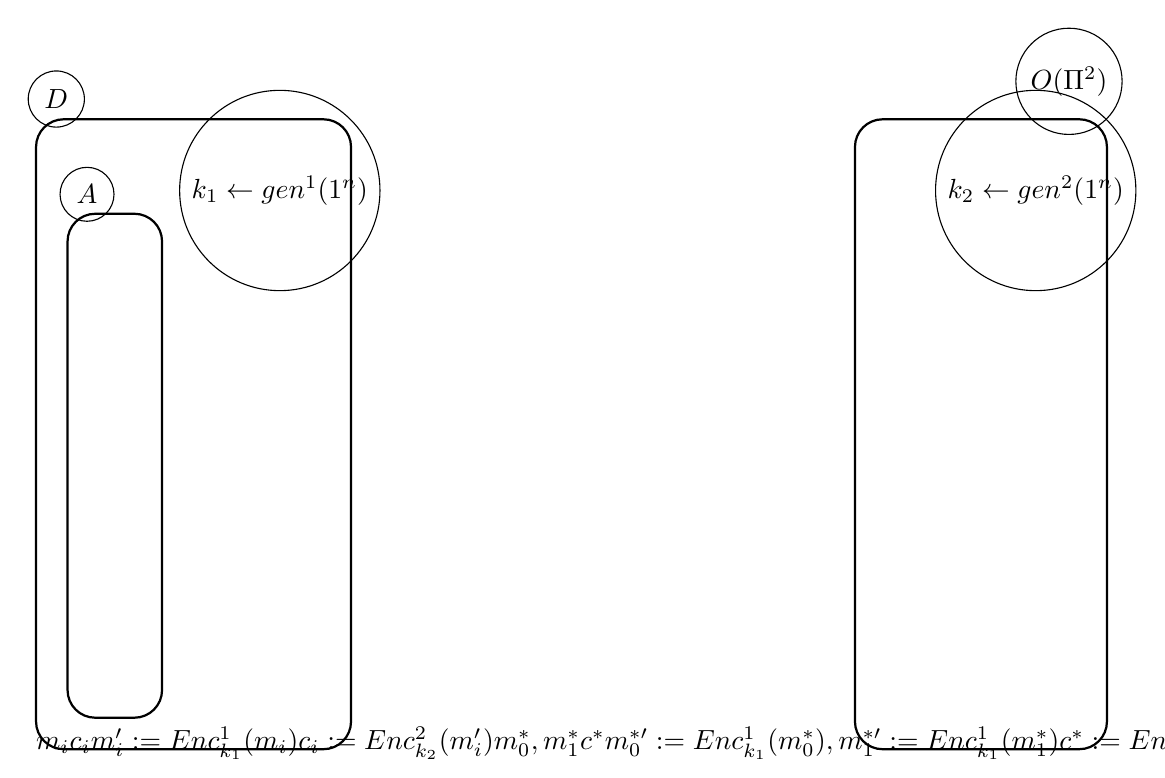
\begin{tikzpicture}[scale=0.8]
			%structure
			\draw[rounded corners=10pt,thick] (0,0) rectangle (5,10);
			\draw[rounded corners=10pt,thick] (0.5,0.5) rectangle (2,8.5);
			\draw[rounded corners=10pt,thick] (13,0) rectangle (17,10);
			\node[above right] at (0,10) {$D$};
			\node[above right] at (0.5,8.5) {$A$};
			\node[above left] at (17,10) {$O(\Pi^2)$};
			\node[below left] at (5,10) {$k_1 \leftarrow gen^1(1^n)$};
			\node[below left] at (17,10) {$k_2 \leftarrow gen^2(1^n)$};
			
			%train phase
			\flect (2,8) -- (4,8) \mess {$m_i$};
			\flect (4,7) -- (2,7) \mess {$c_i$};
			\flect (5,8) -- (13,8) \mess {$m_i':=Enc_{k_1}^1(m_i)$};
			\flect (13,7) -- (5,7) \mess {$c_i:=Enc_{k_2}^2(m_i')$};
			
			%challenge phase
			\flecc (2,5.5) -- (4,5.5) \mess {$m^{\ast}_0,m^{\ast}_1$};
			\flecc (4,4.5) -- (2,4.5) \mess {$c^\ast$};
			\flecc (5,5.5) -- (13,5.5) \mess {$m
			_0^{\ast\prime}:=Enc_{k_1}^{1}(m_0^\ast),m_1^{\ast\prime}:=Enc_{k_1}^{1}(m_1^{\ast})$};
			\flecc (13,4.5) -- (5,4.5) \mess {$c^\ast:=Enc_{k_2}^{2}(m_b^{\ast\prime})$};
			\node[below right] at (13,5.5) {$b \leftarrow \{0,1\}$};
			
			%train phase
			\flect (2,3) -- (4,3) \mess {$m_i$};
			\flect (4,2) -- (2,2) \mess {$c_i$};
			\flect (5,3) -- (13,3) \mess {$m_i':=Enc_{k_1}^1(m_i)$};
			\flect (13,2) -- (5,2) \mess {$c_i:=Enc_{k_2}^2(m_i')$};
			
			% output
			\flec (2,1) -- (3,1) node[pos=1,right] {$b'$};
			\flec (5,1) -- (6,1) node[pos=1,right] {$b''=b'$};
		\end{tikzpicture}
	\end{center}
	As we can see in every case, the distinguisher will have the same probability to find the message encrypted by the oracle than the attacker to break the scheme. As the attacker can only have a probability of $1/2 + \varepsilon$ to succeed the distinguisher will have the same probability. So, the scheme $\Pi$ is secure.
	
	\item As seen in the previous development, if $\Pi^2$ is CPA secure, $\Pi$ is CPA secure. There is no restriction on $\Pi^1$ in that case. Therefore $\Pi^1$ could be such that $Enc^1_{k_1}(m):=m$ which is obviously not CPA secure. So the proposition is false.
	
	\item Idem
	
	\item \textbf{If $\Pi^1$ is CPA secure, is it $\Pi'$ CPA secure?}\\
	The $\Pi'$ scheme is CPA secure if and only if $\Pi^2$ is also CPA secure.
	
	For example, if $Enc_{k_2}^2(m) = m$ then the scheme $\Pi'$ is not CPA secure.
	
	TO DEVELOP. (solution of the teaching assistant?)
	
	\item TODO
	
	\item TODO
	
	\item TODO
\end{enumerate}

\end{solution}


\section{TP 2}
%\addcontentsline{toc}{section}{TP 2}


% \section*{Rappel}

% \begin{center}
% \textbf{Liste des équivalences logiques}
% \end{center}

% \textsf{Lois commutatives}
% \begin{enumerate}
% 	\item $p \vee q \Lleftarrow\!\!\!\!\Rrightarrow q \vee p$ \textit{(commutativité de $\vee$)}
% 	\item $p \wedge q \Lleftarrow\!\!\!\!\Rrightarrow q \wedge p$ \textit{(commutativité de $\wedge$)}
% 	\item $p \Leftrightarrow q \Lleftarrow\!\!\!\!\Rrightarrow q \Leftrightarrow q$ \textit{(commutativité de $\Leftrightarrow$)}
% \end{enumerate}

% \textsf{Lois associatives}
% \begin{enumerate}
% 	\item $(p \vee q) \vee r \Lleftarrow\!\!\!\!\Rrightarrow p \vee (q \vee r)$ \textit{(associativité de $\vee$)}
% 	\item $(p \wedge q) \wedge r \Lleftarrow\!\!\!\!\Rrightarrow p \wedge (q \wedge r)$ \textit{(associativité de $\wedge$)}
% \end{enumerate}

% \textsf{Lois distributives}
% \begin{enumerate}
% 	\item $p \wedge (q \vee r) \Lleftarrow\!\!\!\!\Rrightarrow (p \wedge q) \vee (p \wedge r)$ \textit{(distributivité de $\wedge$ sur $\vee$)}
% 	\item $p \vee (q \wedge r) \Lleftarrow\!\!\!\!\Rrightarrow (p \vee q) \wedge (p \vee r)$ \textit{(distributivité de $\vee$ sur $\wedge$)}
% \end{enumerate}

% \textsf{Lois de De Morgan}
% \begin{enumerate}
% 	\item $\neg(p \wedge q) \Lleftarrow\!\!\!\!\Rrightarrow \neg p \vee \neg q$ \textit{(loi 1 de De Morgan)}
% 	\item $\neg(p \vee q) \Lleftarrow\!\!\!\!\Rrightarrow \neg p \wedge \neg q$ \textit{(loi 2 de De Morgan)}
% \end{enumerate}

% \textsf{Loi de la négation}
% \begin{enumerate}
% 	\item $\neg \neg p \Lleftarrow\!\!\!\!\Rrightarrow p$
% \end{enumerate}

% \textsf{Loi du tiers exclu}
% \begin{enumerate}
% 	\item $p \vee \neg p \Lleftarrow\!\!\!\!\Rrightarrow \textbf{true} $
% \end{enumerate}

% \textsf{Loi de la contradiction}
% \begin{enumerate}
% 	\item $p \wedge \neg p \Lleftarrow\!\!\!\!\Rrightarrow \textbf{false}$
% \end{enumerate}

% \textsf{Loi de l'implication}
% \begin{enumerate}
% 	\item $p \Rightarrow q \Lleftarrow\!\!\!\!\Rrightarrow \neg p \vee q$
% \end{enumerate}

% \textsf{Loi du contraposée}
% \begin{enumerate}
% 	\item $p \Rightarrow q \Lleftarrow\!\!\!\!\Rrightarrow \neg q \Rightarrow \neg p$
% \end{enumerate}

% \textsf{Loi de l'équivalence}
% \begin{enumerate}
% 	\item $p \Leftrightarrow q \Lleftarrow\!\!\!\!\Rrightarrow (p \Rightarrow q) \wedge (q \Rightarrow p)$
% \end{enumerate}

% \textsf{Lois de l'idempotence}
% \begin{enumerate}
% 	\item $p \Lleftarrow\!\!\!\!\Rrightarrow p \vee p$ \textit{(idempotence de $\vee$)}
% 	\item $p \Lleftarrow\!\!\!\!\Rrightarrow p \wedge p$ \textit{(idempotence de $\wedge$)}
% \end{enumerate}

% \textsf{Lois de simplification}
% \begin{enumerate}
% 	\item $p \wedge \textbf{true} \Lleftarrow\!\!\!\!\Rrightarrow p$
% 	\item $p \vee \textbf{true} \Lleftarrow\!\!\!\!\Rrightarrow \textbf{true}$
% 	\item $p \wedge \textbf{false} \Lleftarrow\!\!\!\!\Rrightarrow \textbf{false}$
% 	\item $p \vee \textbf{false} \Lleftarrow\!\!\!\!\Rrightarrow p$
% 	\item $p \vee (p \wedge q) \Lleftarrow\!\!\!\!\Rrightarrow p$
% 	\item $p \wedge (p \vee q) \Lleftarrow\!\!\!\!\Rrightarrow p$
% \end{enumerate}

% \begin{center}
% \textbf{Liste des règles d'inférence}
% \end{center}

% \begin{tabular}{c c c c}

% \textsf{Conjonction} & \textsf{Simplification} & \textsf{Addition} & \textsf{Syllogisme disjoint}   \\

% \begin{tabular}{l}
% $p$ \\
% $q$ \\
% \hline
% $p \wedge q$
% \end{tabular}

% &

% \begin{tabular}{l}
% $p \wedge q$ \\
% \hline
% $p$
% \end{tabular}

% &

% \begin{tabular}{l}
% $p$ \\
% \hline
% $p \vee q$
% \end{tabular}

% &

% \begin{tabular}{l}
% $p \vee q$ \\
% $\neg p$ \\
% \hline
% $q$
% \end{tabular} \\

% \textsf{Modus ponens} & \textsf{Modus tollens} & \textsf{Contradiction} & \textsf{Double négation} \\

% \begin{tabular}{l}
% $p \Rightarrow q$ \\
% $p$ \\
% \hline
% $q$
% \end{tabular}

% &

% \begin{tabular}{l}
% $p \Rightarrow q$ \\
% $\neg q$ \\
% \hline
% $\neg p$
% \end{tabular}

% &

% \begin{tabular}{l}
% $p$ \\
% $\neg p$ \\
% \hline
% $q$
% \end{tabular}

% &
% \begin{tabular}{l}
% $\neg \neg p$ \\
% \hline
% $p$
% \end{tabular} \\

% \textsf{Transitivité} & \textsf{Lois de l'équivalence} & \textsf{Théorème de la déduction} & \textsf{Réduction à l'absurde} \\

% \begin{tabular}{l}
% $p \Leftrightarrow q$ \\
% $q \Leftrightarrow r$ \\
% \hline
% $p \Leftrightarrow r$
% \end{tabular}

% &

% \begin{tabular}{l}
% $p \Leftrightarrow q$ \\
% \hline
% $p \Rightarrow q$ \\
% $q \Rightarrow p$
% \end{tabular}

% &

% \begin{tabular}{l}
% $p, \ldots, r, \boxed{s} \vdash t$ \\
% \hline
% $p, \ldots, r \vdash s \Rightarrow t$
% \end{tabular}

% &

% \begin{tabular}{l}
% $p, \ldots, q, \boxed{r} \vdash s$ \\
% $p, \ldots, q, \boxed{r} \vdash \neg s$ \\
% \hline
% $p, \ldots, q \vdash \neg r$
% \end{tabular}

% \end{tabular}

% \newpage
% \section*{Exercices}

\subsection*{Exercice 1}
Démontrez les équivalences logiques suivantes.

\begin{enumerate}
	\item $p \wedge (q \wedge r)  \Lleftarrow\!\!\!\!\Rrightarrow (p \wedge q) \wedge r$
	\item $p \Rightarrow (q \Rightarrow r) \Lleftarrow\!\!\!\!\Rrightarrow (p \Rightarrow q) \Rightarrow (p \Rightarrow r)$
	\item $p \wedge (p \Rightarrow q) \Rightarrow q \Lleftarrow\!\!\!\!\Rrightarrow \textbf{true}$
	\item $(p \vee q) \wedge (\neg p \vee q) \Lleftarrow\!\!\!\!\Rrightarrow q$
	\item $(p \vee q) \vee (\neg p \wedge \neg q) \Lleftarrow\!\!\!\!\Rrightarrow \textbf{true}$
% 	\item $(p \vee q) \wedge (\neg p \wedge \neg q) \Lleftarrow\!\!\!\!\Rrightarrow \textbf{false}$
	\item $p \vee (q \wedge r) \Lleftarrow\!\!\!\!\Rrightarrow \neg (\neg (p \vee q) \vee \neg (p \vee r))$
	\item $(p \vee q) \wedge \neg (p \wedge q) \Lleftarrow\!\!\!\!\Rrightarrow (p \wedge \neg q) \vee (\neg p \wedge q)$
	\item $p \wedge q \Lleftarrow\!\!\!\!\Rrightarrow (p \vee q) \wedge (p \Leftrightarrow q)$
\end{enumerate}

    \subsubsection*{Solution}
    Notons d'abord que toutes les preuves suivantes peuvent aussi être réalisées grâce aux table de vérités.
\begin{enumerate}
	\item
    \begin{flalign*}
    p \land (q \land r) &\Lleftarrow\!\!\!\!\Rrightarrow \lnot \lnot (p \land ( q \land r )) \tag*{Double négation}\\
    &\Lleftarrow\!\!\!\!\Rrightarrow \lnot ( \lnot (q \land r) \lor \lnot p ) \tag*{De Morgan}\\
    & \Lleftarrow\!\!\!\!\Rrightarrow \lnot ((\lnot r \lor \lnot q) \lor \lnot p) \tag*{De Morgan} \\
    & \Lleftarrow\!\!\!\!\Rrightarrow \lnot(( \lnot p \lor \lnot q) \lor \lnot r) \tag*{Associativité}\\
    & \Lleftarrow\!\!\!\!\Rrightarrow \lnot (\lnot p \lor \lnot q) \land \lnot \lnot r \tag*{De Morgan} \\
    & \Lleftarrow\!\!\!\!\Rrightarrow (p \land q) \land r \tag*{De Morgan et double négation}
    \end{flalign*}

	\item
	\begin{flalign*}
    p \Rightarrow (q \Rightarrow r)& \Lleftarrow\!\!\!\!\Rrightarrow p \Rightarrow (\lnot q \lor r) \tag*{Implication} \\
    & \Lleftarrow\!\!\!\!\Rrightarrow \lnot p \lor (\lnot q \lor r) \tag*{Implication} \\
    & \Lleftarrow\!\!\!\!\Rrightarrow (\lnot p \lor \lnot q) \lor r \tag*{Associativité}\\
    & \Lleftarrow\!\!\!\!\Rrightarrow (\text{true} \land (\lnot p \lor \lnot q)) \lor r \tag*{Simplification inverse} \\
    & \Lleftarrow\!\!\!\!\Rrightarrow ((\lnot p \lor p) \land  (\lnot p \lor \lnot q)) \lor r \tag*{Loi du tiers exclus}\\
    & \Lleftarrow\!\!\!\!\Rrightarrow (\lnot p \lor (p \land \lnot q)) \lor r \tag*{Distributivité}\\
    & \Lleftarrow\!\!\!\!\Rrightarrow ((p \lor \lnot q) \lor \lnot p) \lor r \tag*{Associativité} \\
    & \Lleftarrow\!\!\!\!\Rrightarrow (p \land \lnot q) \lor (\lnot p \lor r) \tag*{Associativité} \\
    & \Lleftarrow\!\!\!\!\Rrightarrow \lnot \lnot (p \land \lnot q) \lor (\lnot p \lor r) \tag*{Double négation} \\
    & \Lleftarrow\!\!\!\!\Rrightarrow \lnot (\lnot p \lor q ) \lor ( \lnot p \lor \lnot r) \tag*{De Morgan}\\
    & \Lleftarrow\!\!\!\!\Rrightarrow (p \Rightarrow q) \Rightarrow (p \Rightarrow r) \tag*{Implication}
    \end{flalign*}

	\item
	\begin{flalign*}
    p \land (p \Rightarrow q ) \Rightarrow q & \Lleftarrow\!\!\!\!\Rrightarrow p \land (\lnot p \lor q ) \Rightarrow q \tag*{Implication} \\
    & \Lleftarrow\!\!\!\!\Rrightarrow \lnot (p \land ( \lnot p \lor q )) \lor q \tag*{Implication}\\
    & \Lleftarrow\!\!\!\!\Rrightarrow \lnot p \lor \lnot ( \lnot p \lor q ) \lor q \tag*{De Morgan}\\
    & \Lleftarrow\!\!\!\!\Rrightarrow \lnot p \lor (p \land \lnot q) \lor q \tag*{De Morgan}\\
    & \Lleftarrow\!\!\!\!\Rrightarrow (( \lnot p \lor p ) \land ( \lnot p \lor \lnot q )) \lor q \tag*{Distributivité}\\
    & \Lleftarrow\!\!\!\!\Rrightarrow (\text{true} \land ( \lnot p \lor \lnot q )) \lor q \tag*{Loi du tiers exclu}\\
    & \Lleftarrow\!\!\!\!\Rrightarrow ( \lnot p \lor \lnot q ) \lor q \tag*{Simplification}\\
    & \Lleftarrow\!\!\!\!\Rrightarrow \lnot p \lor (\lnot q \lor q ) \tag*{Associativité}\\
    & \Lleftarrow\!\!\!\!\Rrightarrow \lnot p \lor \text{true} \tag*{Loi du tiers exclu}\\
    & \Lleftarrow\!\!\!\!\Rrightarrow \text{true} \tag*{Simplification}\\
    \end{flalign*}

	\item
    \begin{flalign*}
    (p \lor q) \land (\lnot p \lor q) & \Lleftarrow\!\!\!\!\Rrightarrow (q \lor p) \land (q \lor \lnot p) \tag*{Loi commutative}\\
    & \Lleftarrow\!\!\!\!\Rrightarrow q \lor (p \land \lnot p) \tag*{Distributivité}\\
    & \Lleftarrow\!\!\!\!\Rrightarrow q \lor \text{false} \tag*{Simplification}\\
    & \Lleftarrow\!\!\!\!\Rrightarrow q \tag*{Simplification}
    \end{flalign*}

	\item
    \begin{flalign*}
    (p \vee q) \vee (\neg p \wedge \neg q) & \Lleftarrow\!\!\!\!\Rrightarrow (p \vee q) \vee \neg ( p \vee q) \tag*{De Morgan} \\
    & \Lleftarrow\!\!\!\!\Rrightarrow \text{true} \tag*{Loi du tiers exclu}
    \end{flalign*}

	\item
    \begin{flalign*}
    \lnot ( \lnot ( p \lor q ) \lor \lnot (p \lor r ) ) & \Lleftarrow\!\!\!\!\Rrightarrow (p \lor q ) \land ( p \lor r) \tag*{De Morgan}\\
    & \Lleftarrow\!\!\!\!\Rrightarrow p \lor ( q \land r ) \tag*{Distributivité}
    \end{flalign*}

	\item
    \begin{flalign*}
    (p \lor q) \land \lnot ( p \land q) & \Lleftarrow\!\!\!\!\Rrightarrow \lnot (\lnot (p \lor q ) \lor (p \land q)) \tag*{Double négation et De Morgan}\\
    & \Lleftarrow\!\!\!\!\Rrightarrow \lnot (( \lnot p \land \lnot q) \lor ( p \land q)) \tag*{De Morgan}\\
    & \Lleftarrow\!\!\!\!\Rrightarrow \lnot ((\lnot p \lor p) \land (\lnot p \lor q) \land (\lnot q \lor p) \land (\lnot q \lor q)) \tag*{Distributivité}\\
    & \Lleftarrow\!\!\!\!\Rrightarrow \lnot (\text{true} \land (\lnot p \lor q) \land (\lnot q \lor p) \land \text{true}) \tag*{Simplification}\\
    & \Lleftarrow\!\!\!\!\Rrightarrow \lnot ((\lnot p \lor q) \land (\lnot q \lor p)) \tag*{Simplification}\\
    & \Lleftarrow\!\!\!\!\Rrightarrow \lnot (\lnot p \lor q) \lor \lnot(\lnot q \lor p) \tag*{De Morgan}\\
    & \Lleftarrow\!\!\!\!\Rrightarrow (p \land \lnot q) \lor ( q \land \lnot p) \tag*{De Morgan}
    \end{flalign*}

	\item
    \begin{flalign*}
    (p \lor q) \land (p \Leftrightarrow q) & \Lleftarrow\!\!\!\!\Rrightarrow (p \lor q) \land (\lnot p \lor q) \land (p \lor \lnot q) \tag*{Double implication + loi de l'équivalence}\\
    & \Lleftarrow\!\!\!\!\Rrightarrow (p \land \lnot p \land p) \lor (p \land \lnot p \land \lnot q) \lor (p \land q \land p) \lor (p \land q \land \lnot q)\\
    & \lor (q \land \lnot p \land p)\lor (q \land \lnot p \land \lnot q) \lor (q \land q \land p) \lor (q \land q \land \lnot q) \tag*{Distributivité}\\
    & \Lleftarrow\!\!\!\!\Rrightarrow \text{false} \lor \text{false} \lor (p \land q \land p) \lor \text{false} \lor \text{false} \lor \text{false} \lor (q \land q \land p) \lor \text{false} \tag*{Simplification}\\
    & \Lleftarrow\!\!\!\!\Rrightarrow (p \land q) \lor (q \land p) \tag*{Simplification}\\
    & \Lleftarrow\!\!\!\!\Rrightarrow (p \land q) \tag*{Simplification}
    \end{flalign*}

\end{enumerate}


\subsection*{Exercice 2}
Démontrez, à l'aide d'une table de vérité, la validité des arguments suivants:

\begin{enumerate}
	\item \enter

	\begin{flushleft}
	\begin{tabular}{l}
		$p \vee q$ \\
		$\neg p$ \\
	\hline
	$q$
	\end{tabular}
\end{flushleft}


	\item \enter

	\begin{flushleft}
	\begin{tabular}{l}
		$p$ \\
		\hline
	$p \vee q$
	\end{tabular}

\end{flushleft}

	\item \enter

	\begin{flushleft}
	\begin{tabular}{l}
		$p \Rightarrow q$ \\
		$q \Rightarrow r$ \\
	\hline
	$p \Rightarrow r$
	\end{tabular}

\end{flushleft}

\end{enumerate}

    \subsubsection*{Solution}

    \begin{enumerate}
    	\item \hspace{1em}

    \begin{center}
	\begin{tabular}{cc|ccc}
		$p$ & $q$ & $\lnot p$ & $p \lor q$ & $(\lnot p) \land (p \lor q)$ \\
		\hline
		T&T&F&T&F\\
		T&F&F&T&F\\
		F&\color{red}T&T&T&\color{red}T\\
		F&F&T&F&F\\
	\end{tabular}
    \end{center}

    On remarque que quand $(\lnot p) \land (p \lor q)$ est vrai, $q$ est vrai.

	\item  \hspace{1em}
    \begin{center}
    	\begin{tabular}{cc|c}
    		$p$ & $q$ & $p \lor q$ \\
    		\hline
    		\color{red}T&T&\color{red}T\\
    		\color{red}T&F&\color{red}T\\
    		F&T&T\\
    		F&F&F\\
    	\end{tabular}
    \end{center}

    On remarque que quand $p$ est vrai, $p \lor q$ est vrai.

	\item  \hspace{1em}
    \begin{center}
    	\begin{tabular}{ccc|cccc}
    		$p$ & $q$ & $r$ & $(p \Rightarrow q)$ & $\land$ & $(q \Rightarrow r)$ & $(p \Rightarrow r)$ \\
    		\hline
    		T&T&T&T&\color{red}T&T&\color{red}T\\
    		T&T&F&T&F&F&F\\
    		T&F&T&F&F&T&T\\
    		T&F&F&F&F&T&F\\
    		F&T&T&T&\color{red}T&T&\color{red}T\\
    		F&T&F&T&F&F&T\\
    		F&F&T&T&\color{red}T&T&\color{red}T\\
    		F&F&F&T&\color{red}T&T&\color{red}T\\
    	\end{tabular}
    \end{center}

    On remarque que quand $(p \Rightarrow q) \land (q \Rightarrow r)$ est vrai, $(p \Rightarrow r)$ est vrai.


\end{enumerate}
\subsection*{Exercice 3}
Démontrez que les arguments suivants ne sont pas valides.

\begin{enumerate}
	\item \enter

	\begin{flushleft}
	\begin{tabular}{l}
		$p \vee q$ \\
		$\neg p$ \\
	\hline
	$\neg q$
	\end{tabular}

\end{flushleft}

	\item \enter

	\begin{flushleft}
	\begin{tabular}{l}
		$p \Leftrightarrow q$ \\
		$p \Rightarrow r$ \\
	$r$ \\
	\hline
	$p$
	\end{tabular}

\end{flushleft}


% 	\item \enter
%
% 	\begin{flushleft}
% 	\begin{tabular}{l}
% 		$p \vee q$ \\
% 		$q$ \\
% 	\hline
% 	$p$
% 	\end{tabular}
%
% \end{flushleft}

	\item \enter

	\begin{flushleft}
	\begin{tabular}{l}
		$p \Rightarrow q$ \\
		$q \Rightarrow p$ \\
	\hline
	$p \wedge q$
	\end{tabular}

\end{flushleft}

% 	\item \enter
%
% 	\begin{flushleft}
% 	\begin{tabular}{l}
% 		$p \Rightarrow q$ \\
% 		$q$ \\
% 	\hline
% 	$p$
% 	\end{tabular}
% \end{flushleft}

\end{enumerate}

    \subsubsection*{Solution}
    Il y a deux façons de résoudre cet exercice.
    Nous faisons avec le premier un exemple de ces deux méthodes.
\begin{enumerate}
	\item
    Tout d'abord, l'algorithme de preuve :

    \begin{center}
    \begin{tabular}{|l|l|}
    \hline
    1. $p \lor q$ & Prémisse \\
    2. $\lnot p$ & Prémisse \\
    \hspace{0.5cm} 3. $\lnot q$ & Hypothèse \\
    \hspace{0.5cm} 4. $p$ & Syllogisme disjoint (1, 3) \\
    5. $q$ & Réduction à l'absurde \\
    \hline
    \end{tabular}
    \end{center}

    Ensuite une table de vérité :

    \begin{center}
    	\begin{tabular}{cc|ccc|c}
    		$P$ & $Q$ & $(P \lor Q) $ & $\land$ & $\neg P$ & $\neg Q$ \\
    		\hline
    		T & T & T & F & F & F\\
    		T & F & T & F & F & T\\
    		F & T & T & \color{red}T & T & \color{red}F\\
    		F & F & F & F & T & T\\
    	\end{tabular}
    \end{center}

    On constate que lorsque $(P \lor Q) \land \neg P$ est vrai, $\neg Q$ est faux.

	\item
    Il suffit de trouver une interprétation où c'est faux. Ici on peut prendre :

    \begin{flalign*}
    VAL_{I}(p) &= \text{false}\\
    VAL_{I}(q) &= \text{false}\\
    VAL_{I}(r) &= \text{true}\\
    \end{flalign*}

    Les prémisses sont vraies, pas la conclusion.

	\item
    Il suffit de trouver une interprétation où c'est faux. Ici on peut prendre :

    \begin{flalign*}
    VAL_{I}(p) &= \text{false}\\
    VAL_{I}(q) &= \text{false}\\
    \end{flalign*}

    Les prémisses sont vraies, pas la conclusion.
\end{enumerate}

\subsection*{Exercice 4}
Pour chaque ensemble de prémisses, démontrez la conclusion qui suit. Faites attention à bien identifier les
lois logiques et les règles d'inférence utilisées.
\begin{enumerate}

% \item Premisses: $A \vee B \vee C, \ \neg A, \ \neg B$ \\
% 			Conclusion: $C$
% \item Premisses: $(p \wedge q) \vee r$ \\
%       Conclusion: $\neg q \Rightarrow r$
\item Premisses: $p \Rightarrow q$, \ $q \Rightarrow r$ \\
      Conclusion: $p \Rightarrow r$
\item Premisses: $p \Rightarrow q$, \ $r \Rightarrow t$, \ $q \vee t \Rightarrow u$, \ $\neg u$ \\
      Conclusion: $\neg p \wedge \neg r$
\item Premisses: $\neg p \Rightarrow (q \Rightarrow r)$, \ $t \vee \neg r \vee u$, \ $p \Rightarrow t$, \ $\neg t$ \\
      Conclusion: $q \Rightarrow u$
% \item Premisses: $A \Rightarrow B, \ C \Rightarrow D, \ (B \vee D) \Rightarrow E, \ \neg E$ \\
% 			Conclusion: $\neg A \wedge \neg C$


\item Premisses: $p \Rightarrow \neg q, \ q \vee r \vee s, \ \neg r \vee s \Rightarrow p, \ \neg r$  \\
			Conclusion: $s$


\item Premisses: $\neg p \Rightarrow (q \Rightarrow r), \ s \vee \neg r \vee t, \ p \Rightarrow s, \ \neg s$ \\
			Conclusion: $q \Rightarrow t$


%   \item Premisses: $p \wedge q$ \\
%        ronclusion: $p \vee q$
%  \item Premisses: $(p \wedge q) \vee r$ \\
%        ronclusion: $r \vee q$
 \item Premisses: $\neg ( \neg p \wedge q), \ \neg (\neg q \vee r)$ \\
       Conclusion: $p$
%  \item Premisses: $p \vee q$ \\
%        ronclusion: $p \vee \neg \neg q$
 \item Premisses: $p \vee q, \ \neg q \vee r$ \\
       Conclusion: $p \vee r$
 \item Premisses: $(p \wedge q) \vee (r \wedge s), \ (q \wedge r) \vee (s \wedge t)$ \\
       Conclusion: $r \vee (p \wedge t)$

\end{enumerate}

    \subsubsection*{Solution}
    \begin{enumerate}

    %%% 4.1 %%%
	\item  \hspace{1em}
    \begin{center}
    \begin{tabular}{|l|l|}
    \hline
    1. $p \Rightarrow q$ & Prémisse \\
    2. $q \Rightarrow r$ & Prémisse \\
    \hspace{0.5cm} 3. $p$ & Hypothèse \\
    \hspace{0.5cm} 4. $q$ & Modus ponens (1, 3) \\
    \hspace{0.5cm} 5. $r$ & Modus ponens (2, 4) \\
    6. $p \Rightarrow r$ & Théorème de déduction (3, 5) \\
    \hline
    \end{tabular}
    \end{center}

    %%% 4.2 %%%
	\item  \hspace{1em}
    \begin{center}
    \begin{tabular}{|l|l|}
    \hline
    1. $p \Rightarrow q$ & Prémisse \\
    2. $r \Rightarrow t$ & Prémisse \\
    3. $q \lor t \Rightarrow u $ & Prémisse \\
    4. $\lnot u$ & Prémisse \\
    5. $\lnot (q \lor t)$ & Modus tollens (3, 4) \\
    6. $\lnot q \land \lnot t$ & De Morgan (5) \\
    7. $\lnot t$ & Simplification (6) \\
    8. $\lnot r$ & Modus tollens (2, 7) \\
    9. $\lnot q$ & Simplification (6) \\
    10. $\lnot p$ & Modus tollens (1, 9) \\
    11. $\lnot r \land \lnot p$ & Conjonction (8, 10) \\
    \hline
    \end{tabular}
    \end{center}

    %%% 4.3 %%%
	\item  \hspace{1em}
    \begin{center}
    \begin{tabular}{|l|l|}
    \hline
    1. $\lnot p \Rightarrow (q \Rightarrow r)$ & Prémisse \\

    2. $t \lor \lnot r \lor u$ & Prémisse \\
    3. $p \Rightarrow t$ & Prémisse \\
    4. $\lnot t$ & Prémisse \\
    5. $\lnot p$ & Modus tollens (3, 4) \\
    6. $q \Rightarrow r$ & Modus ponens (1, 5) \\
    7. $\lnot r \lor u$ & Syllogisme disjoint (2, 4) \\
    \hspace{0.5cm} 8. $q$ & Hypothèse \\
    \hspace{0.5cm} 9. $r$ & Modus ponens (6, 8) \\
    \hspace{0.5cm} 10. $u$ & Syllogisme disjoint (7,9) \\
    11. $q \Rightarrow u$ & Déduction (8, 10) \\
    \hline
    \end{tabular}
    \end{center}

    %%% 4.4 %%%
	\item  \hspace{1em}
    \begin{center}
    \begin{tabular}{|l|l|}
    \hline
    1. $p \Rightarrow \lnot q$ & Prémisse \\
    2. $q \lor r \lor s$ & Prémisse \\
    3. $\lnot r \lor s \Rightarrow p$ & Prémisse \\
    4. $\lnot r$ & Prémisse \\
    5. $q \lor s$ & Syllogisme disjoint (2, 4) \\
    6. $\lnot r \lor s$ & Addition(4) \\
    7. $p$ & Modus ponens (3, 6) \\
    8. $\lnot q$ & Modus ponens (1, 7) \\
    9. $s$ & Syllogisme disjoint (5, 8) \\
    \hline
    \end{tabular}
    \end{center}

    %%% 4.5 %%%
	\item  \hspace{1em}
    \begin{center}
    \begin{tabular}{|l|l|}
    \hline
    1. $\lnot p \Rightarrow (q \Rightarrow r)$ & Prémisse \\
    2. $s \lor \lnot r \lor t$ & Prémisse \\
    3. $p \Rightarrow s$ & Prémisse \\
    4. $\lnot s$ & Prémisse \\
    5. $\lnot p$ & Modus tollens (3, 4) \\
    6. $q \Rightarrow r$ & Modus ponens (1, 5) \\
    7. $\lnot r \lor t$ & Syllogisme disjoint (2, 4) \\
    \hspace{0.5cm} 8. $q$ & Hypothèse \\
    \hspace{0.5cm} 9. $r$ & Modus ponens (6, 8) \\
    \hspace{0.5cm} 10. $t$ & Syllogisme disjoint (7,9) \\
    11. $q \Rightarrow t$ & Déduction (8, 10) \\
    \hline
    \end{tabular}
    \end{center}

    %%% 4.6 %%%
	\item  \hspace{1em}
    \begin{center}
    \begin{tabular}{|l|l|}
    \hline
    1. $\lnot ( \lnot p \land q)$ & Prémisse \\
    2. $\lnot ( \lnot q \lor r)$ & Prémisse \\
    3. $p \lor \lnot q$ & De Morgan (1) \\
    4. $q \land \lnot r$ & De Morgan (2) \\
    5. $q$ & Simplification (4) \\
    6. $p$ & Syllogisme disjoint (3, 5) \\
    \hline
    \end{tabular}
    \end{center}

    %%% 4.7 %%%
	\item  \hspace{1em}
    \begin{center}
    \begin{tabular}{|l|l|}
    \hline
    1. $p \lor q$ & Prémisse \\
    2. $\lnot q \lor r$ & Prémisse \\
    3. $q \Rightarrow r$ & Loi de l'implication (2) \\
    \hspace{0.5cm} 4. $\lnot(p \lor r)$ & Hypothèse \\
    \hspace{0.5cm} 5. $\lnot p \land \lnot r$ & De Morgan (4) \\
    \hspace{0.5cm} 6. $\lnot p$ & Simplification (5) \\
    \hspace{0.5cm} 7. $\lnot r$ & Simplification (5) \\
    \hspace{0.5cm} 8. $q$ & Syllogisme disjoint (1, 6) \\
    \hspace{0.5cm} 9. $\lnot q$ & Syllogisme disjoint (2, 7) \\
    10. $p \lor r$ & Réduction à l'absurde (4)\\
    \hline
    \end{tabular}
    \end{center}

    %%% 4.8 %%%
	\item  \hspace{1em}
    \begin{center}
    \begin{tabular}{|l|l|}
    \hline
    1. $(p \land q) \lor (r \land s)$ & Prémisse \\
    2. $(q \land r) \lor (s \land t)$ & Prémisse \\
    3. $(p \lor r) \land (p \lor s) \land (q \lor s) \land (q \lor r)$ & Distributivité (1) \\
    4. $(q \lor s) \land (q \lor t) \land (r \lor s) \land (r \lor t)$ & Distributivité (2) \\
    5. $p \lor r$ & Simplification (3) \\
    6. $r \lor t$ & Simplification (4) \\
    7. $(p \lor r) \land (r \lor t)$ & Conjonction (5, 6) \\
    8. $r \lor (p \land t)$ & Distributivité (7) \\
    \hline
    \end{tabular}
    \end{center}
\end{enumerate}

\subsection*{Exercice 5}
Pour chaque ensemble de prémisses, démontrez la conclusion qui suit. Faites attention à bien identifier les
lois logiques et les règles d'inférence utilisées.
\begin{enumerate}
\item Premisses: \\
      Conclusion: $p \vee \neg (p \wedge q)$
\item Premisses: \\
      Conclusion: $(p \wedge q) \vee \neg p \vee \neg q$
\item Premisses: \\
      Conclusion: $\neg p \vee \neg (\neg q \wedge (\neg p \vee q))$
\end{enumerate}

    \subsubsection*{Solution}
    \begin{enumerate}

	\item  \hspace{1em}
    \begin{center}
    \begin{tabular}{|l|l|}
    \hline
    \hspace{0.5cm} 1. $\neg p$ & Hypothèse \\
    \hspace{0.5cm} 2. $\neg p \lor \neg q$ & Addition (1) \\
    \hspace{0.5cm} 3. $\neg \neg(\neg p \lor \neg q)$ & Négation (2) \\
    \hspace{0.5cm} 4. $\neg(p \land q)$ & De Morgan (3)\\
    5. $\neg p \Rightarrow \neg(p \land q)$ & Déduction (1, 4) \\
    6. $\neg \neg p \lor \neg(p \land q)$ & Implication (5)\\
    7. $p \lor \neg(p \land q)$ & Double négation (6)\\
    \hline
    \end{tabular}
    \end{center}

	\item  \hspace{1em}
    \begin{center}
    \begin{tabular}{|l|l|}
    \hline
    \hspace{0.5cm} 1. $\neg (p \land q)$ & Hypothèse \\
    \hspace{0.5cm} 2. $\neg p \lor \neg q$ & De Morgan (1) \\
    3. $\neg (p \land q) \Rightarrow (\neg p \lor \neg q)$ & Déduction (1, 2) \\
    4. $(\neg \neg(p \land q)) \lor (\neg p \lor \neg q)$ & Implication (3) \\
    5. $(p \land q) \lor (\neg p \lor \neg q)$ & Double négation (4) \\
    \hline
    \end{tabular}
    \end{center}

	\item  \hspace{1em}
    \begin{center}
    \begin{tabular}{|l|l|}
    \hline
    \hspace{0.5cm} 1. $p$ & Hypothèse \\
    \hspace{0.5cm} 2. $p \lor q$ & Addition (1) \\
    \hspace{0.5cm} 3. $(\neg p \lor q) \Leftrightarrow q$ & ex. 2.1 \\
    \hspace{0.5cm} 4. $((\neg p \lor q) \land \neg q) \Leftrightarrow (q \land \neg q)$ & Mystification \\
    \hspace{0.5cm} 5. $\neg ((\neg p \lor q) \land \neg q)$ & Contradiction \\
    6. $p \Rightarrow \neg ((\neg p \lor q) \land \neg q)$ & Déduction (1, 5) \\
    7. $\neg p \lor \neg ((\neg p \lor q) \land \neg q)$ & Implication (6) \\
    \hline
    \end{tabular}
    \end{center}

    \end{enumerate}

\section{}
\subsection{Exercise 1 (Blue-ray security)}
\copypaste{2}{7}

\subsection{Exercise 2 (Authenticated encryption)}
Let $\Pi = \langle \Gen, \Enc, \Dec\rangle$ be an authenticated encryption
scheme such that $\Enc$ encrypts messages of $n$ bits.
%
Do the following systems provide authenticated encryption?  For those
that do, briefly explain why.  For those that do not, present an
attack that breaks one of the security properties of an authenticated
encryption scheme.

\begin{enumerate}
	\item $\Pi' = \langle \Gen, \Enc', \Dec'\rangle$ with
	$\Enc'_k(m) = (\Enc_k(m), \Enc_k(m \oplus (0^{n-1}\|1)))$ and
	$\Dec'_k(c_1, c_2) = \Dec_k(c_1)$ if
	$\Dec_k(c_1) \oplus \Dec_k(c_2) = 0^{n-1}\|1$ and $\bot$ otherwise.

	\item $\Pi' = \langle \Gen, \Enc', \Dec'\rangle$ with
	$\Enc'_k(m) = (\Enc_k(m), \Mac_k(m))$ and $\Dec'_k(c_1, c_2) = \Dec_k(c_1)$
	
	if $\Vrfy_k(\Dec_k(c_1), c_2)=1$ and $\bot$ otherwise. Here, $\Mac$
	and $\Vrfy$ are deterministic algorithms that are part of a secure
	MAC scheme that is compatible with $\Gen$.

\end{enumerate}

\begin{solution}
$\Pi := \langle \text{Gen, Enc, Dec} \rangle$ is an authenticated encryption scheme (AE) if it is CCA-secure and unforgeable.
\begin{enumerate}
    \item The system $\Pi'$ is not AE because it is \textbf{forgeable} and we can show it with this example. If the adversary A asks for the message $m$ ($m'$ corresponds to the message m with the last bit changed) to the oracle access, he will receive the cipher text $(c_1, c_2)$, where $c_1 = Enc_k(m)$ and $c_2 = Enc_k(m\xor 0^{n-1}||1) = Enc_k(m')$ . 
    
    If $\A$ outputs the pair (m',$(c_2, c_1)$), this is a forgery. 
    
    $Dec_k'(c_2,c_1) = Dec_k(c_2) = Dec_k(Enc_k(m')) = m' \neq \perp $ because $Dec_k(c_2) \oplus Dec_k(c_1) = m' \oplus m = m \oplus 0^{n-1}||1 \oplus m = 0^{n-1}||1 $. And $m'$ has not been requested before.
    
    Then we have EncForge$_{A, \Pi'}$(n) = 1  and Pr[EncForge$_{A, \Pi'}$(n)] = 1. $\Pi'$ is then forgeable and it is not an AE. 
    \newline
    With the same technique, an adversary can break the CCA-security of this scheme by querying two different messages $m_1$ and $m_2$, obtaining their encryption, sending \newline
    ($m'_1,m'_2$) = ($m_1 \oplus 0^{n-1}||1, m_2 \oplus 0^{n-1}||1$) for the challenge, and compare the encryption of $m'_b$ with the two previously received ciphertexts.
    \item The sytem $\Pi'$ is not AE because it is not \textbf{CCA-secure} and we can show it because $Mac_k(m)$ does not assure any security (only authentication). So if We use as Mac : 
    $$ Mac_k(m) = m||Mac'_k(m) $$
    It is a good mac but it is trivial to show that is does not hold $CCA-Secure$. $\Pi'$ is then not an AE.
\end{enumerate}
\end{solution}

\subsection{Exercise 3 (Euclidean algorithm for gcd)}
Let $a,b \in \mathbb{Z}$ , $b \neq 0$, consider the following algorithm, presented in Algorithm~\ref{algo:gcd}. ($r=a \% b$ means that $a=qb+r$ where $q$ is the quotient and $r$ is the remainder).

Prove that $x$, the value returned by Algorithm~\ref{algo:gcd}, is $\mathsf{gcd} (a,b)$.

Hint:
\begin{itemize}
\item Prove that $x$ divides  $ \mathsf{gcd} (a,b)$
\item Prove that $ \mathsf{gcd} (a,b)$ divides $x$
\end{itemize}

\begin{algorithm}
	\KwIn{$a$, $b$}
	\KwOut{$\mathsf{gcd}(a,b)$}
	
	\While{ $b\neq 0$}
	{
		$r \leftarrow a\%b$\;
		
		$a \leftarrow b$\;	
		
		$b \leftarrow r$\;	
	}
	\Return($a$)
	
\caption{The Euclidean $\mathsf{gcd}$ algorithm.}\label{algo:gcd}
\end{algorithm}
\begin{solution}
According to the algorithm, we will have as successive value for the different remainder : 
$$ (r_2 = r_0 \% r_1, r_3 = r_1 \% r_2, \ r_4 = r_2 \% r_3, \ ... \ , r_n =  r_{n-2} \% r_{n-1})$$
Where $r_0 = a$, $r_1 = b$ and $r_n$ is the last non null remainder. Then we have the property that :
$$ gcd(r_{i}, r_{i+1}) = gcd(r_{i+1}, r_{i+2}) \ \forall i : \ 0 \leq i \leq n - 2 $$
Otherwise if it was not the case, $\exists i < n $ such that $r_i = 0$. But as $r_n$ is the last non null remainder, we prove by contradiction this property.

As $gcd(r_{n-1}, r_n) = r_n $ because $r_n | r_{n-1}$ (since $r_{n+1} = r_{n-1} \% r_n = 0$), we can conclude that 
$$ gcd(r_0, r_1) = gcd(a, b) = gcd(r_{n-2}, r_{n-1}) = r_n$$
We have proved the value returned by the algorithm is the $gcd(a,b)$
\end{solution}

\subsection{Exercise 4}
Consider the group $\mathbb{Z}^{\ast}_{17}$.
\begin{enumerate}
\item Compute $5^{-1}$.
\item Compute $3^2$, $3^3$ and $3^4$.
\item Does $3$ generate the group?
\item Find $\log_{7}(11)$.
\end{enumerate}
\begin{solution}
Here because p is not too big, it is possible to evaluate "quickly" and "intuitively" the solutions. If it is too hard, there is an algorithm in the slides. 
\begin{enumerate}
    \item Because 35 mod 17 = 1, and $5 \cdot 7 = 35$. \newline Then $5^{-1} = 7$.  ($5 \cdot 7 = 1 \text{ (mod 17)}$)
    \item \begin{itemize}
        \item $3^2 = 9 \text{ (mod 17)}$
        \item $3^3 = 3^2 \cdot 3 = 27 \text{ (mod 17)} = 10 \text{ (mod 17)}$
        \item $3^3 = 3^3 \cdot 3 = 30 \text{ (mod 17)} = 13 \text{ (mod 17)}$
    \end{itemize}
    \item According to \textit{Fermat's little theorem}, if ord(g) = i then if $i|m = |G|$, where G is the commutative group. To see if 3 generate the group, we have to check if $3^i \neq 1$ where $i$ are the divisor of $(p-1) = 16$ (except 16 of course !).
    \begin{itemize}
        \item $3^1$ = 3 mod 17 (trivial)
        \item $3^2$ = 9 mod 17 (evaluated previously)
        \item $3^4$ = 13 mod 17 (evaluated previously)
        \item $3^8$ = $(3^4)^2$ = $(13)^2 \text{ (mod 17)}$ = $(-4)^2 \text{ (mod 17)}$ = 16 mod 17
    \end{itemize}
    We can see that 3 is a generator of the group. 
    
    \textbf{P.S.} : The trick here is to remember the property of the modulo operation here in a $Z^*_p$:
    $$ x = -(p - x) \text{ (mod p)} $$  
    It can make a lot of computing easier (it can become a real pain in the ass).
    \item Here we have to find x such that : 
    $$ 7^x = 11 \text{ (mod 17)} $$
    After (boring) computations, we have here :
    \begin{itemize}
        \item $7^1$ = 7 mod 17
        \item $7^2$ = 15 mod 17 = -2 mod 17
        \item $7^3$ = -14 mod 17 = 3 mod 17
        \item $7^4$ = 4 mod 17
        \item $7^5$ = 11 mod 17 (Bingo)
    \end{itemize}
    Then $log_7(11)$ = 5
\end{enumerate}
\end{solution}

\subsection{Exercise 5 (Group order)}
In this exercise we consider the group $\mathbb{Z}_{59}^*$.

\begin{enumerate}
	\item What is the order of $58$?
	\item What are the possible orders of an element of this group?
	\item Find an element of order more than $20$.
	
\end{enumerate}
\begin{solution}
The order of $g \in \mathbb{Z}^*_{59}$ is the smallest $i$ where $g^i = 1$ 
\begin{enumerate}
    \item ord(58) = 2 because :
    \begin{itemize}
        \item  $58^1$ = 58 mod 59 = -1 mod 59
        \item  $58^2$ = -58 mod 59 = 1 mod 59
    \end{itemize}
    \item According to \textit{Fermat's little theorem}, the possible orders of a group $\mathbb{Z}^*_{p}$ are the divisor of p-1. Then, the possible orders are : 
    \begin{itemize}
        \item 1
        \item 2
        \item 29
        \item 58
    \end{itemize}
    \item The best strategy here is to find a number g where 
    $$ ord(g) > 2 $$
    (To assure you this is correct, just look at the possible ordrers).  \newline
    2 is a correct candidate. 
\end{enumerate}
\end{solution}

\subsection{Exercise 6 (Decisional Diffie-Hellman and \texorpdfstring{$\mathbb{Z}_p^\ast$}{Zp*})}
\label{subsec:4.6}
The goal of this exercise is to show that in some groups DDH and CDH assumptions are conjectured not equivalent, as DDH is easy whereas CDH is conjectured to be hard.

\begin{enumerate}
	\item For all element $a$ of $\mathbb{Z}_{11}^*$, compute $a^2 \mod 11$.
	
	For a prime number $p$, we denote $QR_p$ the set $\{x \in \mathbb{Z}_{p}^* \; | \; \exists a\in \mathbb{Z}_{p}^*, a^2=x\}$, such $x$ are called quadratic residues modulo $p$. Show that if $p$ is odd then $|QR_p|=\frac{p-1}{2}$.
	
		\item For all element $a$ of $\mathbb{Z}_{11}^*$, compute $a^5 \mod 11$. Show that for any odd prime $p$, $x \in QR_p \Leftrightarrow x^{\frac{p-1}{2}}= 1 \mod p$, and that $x \not \in QR_p \Leftrightarrow x^{\frac{p-1}{2}}= -1 \mod p$.
	
	\item Show that $2$ is a generator of $\mathbb{Z}_{11}^*$. For the following pairs $(a,b)$, compute $g^a, g^b$ and $g^{ab}$ in $\mathbb{Z}_{11}^*$ where $g=2$:
	\begin{itemize}
		\item $(2,8)$,
		\item $(1,4)$,
		\item $(3,5)$.
	\end{itemize}
    Show that for $p$ an odd prime, $g^{ab} \not \in QR_p \Leftrightarrow g^a \not \in QR_p \text{ and } g^b \not \in QR_p$.
	
	\item Show that DDH does not hold in $\mathbb{Z}_{p}^*$ with $p$ an odd prime.
\end{enumerate}
\begin{solution}
For this exercise we will work with $\Z_{11}^* = \{1,2,3,4,5,6,7,8,9,10\}$
\begin{enumerate}
    \item 
		For all element $a$ of $\Z_{11}^*$, I've calculated $a^2$ mod $11$.
		$$1^2 = 1 \quad 2^2 = 4 \quad 3^2 = 9 \quad 4^2 = 5 \quad 5^2 = 3 \quad 6^2 = 3 \quad 7^2 = 5 \quad 8^2 = 9 \quad 9^2 = 4 \quad 10^2 = 1$$
		We see that with $p$ odd, we have $\left|QR_p\right| = \frac{p-1}{2}$. We can show it with this development:
		
	\item
		For all element $a$ of $\Z_{11}^*$, I've calculated $a^5$ mod $11$.
		$$1^5 = 3^5 = 4^5 = 5^5 = 9^5 = 1 \qquad 2^5 = 6^5 = 7^5 = 8^5 = 10^5 = 10$$
		We can see that for $p$ prime, we have $x \in QR_p \Leftrightarrow x^{\frac{p-1}{2}} = 1 \mod p$ and  $x \notin QR_p \Leftrightarrow x^{\frac{p-1}{2}} = p-1 \mod p$.
		\begin{itemize}
			\item $x \in QR_p \Leftrightarrow x^{\frac{p-1}{2}} = 1 \mod p$:\\
			We know that $$x \in QR_p \Leftrightarrow \exists a \st x = a^2 \mod p$$
			So we have now $$x = a^2 \mod p \Leftrightarrow x^{\frac{p-1}{2}} = 1 \mod p$$
			If we replace $x$ by $a$ we obtain $a^{2^{(\frac{p-1}{2})}} = 1 \mod p$.\\ 
			But also more simply $a^{p-1} = 1 \mod p$ which is true by the group theory.
			\item $x \notin QR_p \Leftrightarrow x^{\frac{p-1}{2}} = p-1 \mod p$:\\
			We know that $$x \notin QR_p \Leftrightarrow \exists a \st x = a^{1+2n} \mod p$$
			So we have now $$x = a^{1+2n} \mod p \Leftrightarrow x^{\frac{p-1}{2}} = -1 \mod p$$
			We replace $x$ by $a$ and we get $$a^{\frac{p-1}{2}} a^{n(p-1)} \mod p = -1 \mod p$$ 
			We know that $ a^{n(p-1)} \mod p = 1$, thus we simplify the equation like $$a^{\frac{p-1}{2}} \mod p = -1 \mod p$$ 
			We know that $g = a^{\frac{p-1}{2}} \mod p \ne 1 \mod p$ but $g^2 = a^{p-1} = 1 \mod p$. The only solution of these two equations is $g = -1 \mod p$ which is equivalent to $$x^{\frac{p-1}{2}} = p-1 \mod p$$
		\end{itemize}
	
	\item
		The number $2$ is a generator of $\Z_{11}^*$, because ord($2$) $= 10$. In fact, we have $2^1 = 2$, $2^2 = 4$, $2^5 = 10$ and $2^10 = 1$. (Fermat's little theorem)
		We have $g = 2$ so:
		\begin{itemize}
			\item $(2,8):\quad g^2 = 4$, $g^8 = 3$ and $g^{16} = -2$ 
			\item $(1,4):\quad g^1 = 2$, $g^4 = 5$ and $g^{4} = 5$
			\item $(3,5):\quad g^3 = -3$, $g^5 = -1$ and $g^{15} = -1$ TODO
		\end{itemize}
		We have to show that $g^{ab} \notin QR_p \Leftrightarrow g^a \notin QR_p \text{ and } g^b \notin QR_p$.\\
		We know by the definition of the $QR_p$ set that
		$$g^n \notin QR_p \Leftrightarrow \exists m \st n = 2m+1$$
		We can thus extract from $g^{ab} \notin QR_p$ that $\exists m \st ab = 2m+1$.
	    
	    % not necessary
		%We can do a proof by contradiction:\newline 
		%If $a = 2v$ then $ab = 2bv$ and can not be equal to $2m + 1$.\\
		%If $b = 2v$ then $ab = 2av$ and can not be equal to $2m + 1$.\\
		
		So we are assured that $a$ and $b$ are not pairs, so we have the relation $g^a \notin QR_p \text{ and } g^b \notin QR_p$ if and only if $ab = 2m+1$ which is equivalent to $g^{ab} \notin QR_p$. That was what we had to proof.
		
	\item
		We have to show that DDH does not hold in $\Z_p^*$ with p an odd prime number.
		
		We define an attacker that can see $p$, $g$, $g^a$, $g^b$ and receive $h_b = g^{ab}$ or $g^z$.\\ 
		The attitude of the attacker will be this one:
		\begin{itemize}
			\item It receives $g^a \notin QR_p$ and $g^b \notin QR_p$:\\
				It will answer in function of $h_b$:
				\begin{itemize}
					\item $h_b \notin QR_p$:\\
						It answers $h_b = g^{ab}$
					\item $h_b \in QR_p$:\\
						It answers $h_b = g^z$
				\end{itemize}
			\item It receives $g^a \in QR_p$ or $g^b \in QR_p$:\\
				It answers randomly.
		\end{itemize}
		We can identify four cases with their chances of success and appearance (we already know that $\left|QR_p\right|$ is of size $\frac{p-1}{2}$):
		\begin{enumerate}[a)]
			\item $g^a \in QR_p$ or $g^b \in QR_p$ appears $3/4$ of the time with success = $1/2$.
			\item $g^a \notin QR_p$ and $g^b \notin QR_p$ with $h_b = g^{ab}$  appears $1/8$ of the time with success = $1$.
			\item $g^a \notin QR_p$ and $g^b \notin QR_p$ with $h_b = g^z$ and $g^z \in QR_p$  appears $1/16$ of the time with success = $1$.
			\item $g^a \notin QR_p$ and $g^b \notin QR_p$ with $h_b = g^z$ and $g^z \notin QR_p$  appears $1/16$ of the time with success = $0$.
		\end{enumerate}
		We can now recalculate the expected value of success of our attacker:
		$$\begin{array}{rcl}
			\mathbb{E}(success) &=& \frac{3}{4}\cdot \frac{1}{2} +  \frac{1}{8}\cdot 1 + \frac{1}{16}\cdot 1 + \frac{1}{16}\cdot 0\\
								&=& \frac{1}{2} + \frac{1}{16}
		\end{array}$$
		This attacker has one sixteenth of probability more than one half which is not a negligible function (in fact it is a constant function). It is not DDH secure.
\end{enumerate}
\end{solution}
\section{TP 4}
%\addcontentsline{toc}{section}{TP 4}


% \newpage

% \section*{Rappel}

% \textbf{Forme normale conjonctive (FNC):} \\

% $$
% \bigwedge_{i = 1}^n \bigvee_{j = 1}^{m_i} L_{ij}
% $$

% avec $L_{ij}$ litéral, cet-à-dire, une proposition primaire (ex. $A$) ou sa négation (ex. $\neg A$). \\

% \textbf{Example:}

% $$
% (\neg A \vee B) \wedge (B \vee C) \wedge (\neg B \vee C \vee \neg D)
% $$

% \vspace{0.5cm}

% \textbf{Algorithme de normalisation:} \\

% \begin{enumerate}
%  \item Eliminer les $\Rightarrow$ et $\Leftrightarrow$ en les remplaçant par des formules équivalentes a l'aide des lois de l'implication et
%  de l'équivalence. 
%  $$
%  p \Rightarrow q \loeq \neg p \vee q \quad \text{et} \quad p \Leftrightarrow q \loeq (p \Rightarrow q) \wedge (q \Rightarrow p)
%  $$
 
%  \item Déplacer les négations vers l'intérieur et utilisant les lois de De Morgan.
 
%  \item Déplacer les disjonctions ($\vee$) vers l'intérieur en utilisant les lois distributives.
 
%  \item Simplifier en éliminant les formes ($P \vee \neg P$) dans chaque disjonction.
 
% \end{enumerate}

% \vspace{0.5cm}

% \textbf{Règle de résolution:} \\

% \begin{tabular}{l}
% $p_1 \vee p_2 \vee \ldots \vee p_{i - 1} \vee c \vee p_{i + 1} \vee \ldots \vee p_n$ \\
% $q_1 \vee q_2 \vee \ldots \vee q_{j - 1} \vee \neg c \vee q_{j + 1} \vee \ldots \vee q_m$ \\
% \hline
% $p_1 \vee \ldots \vee p_{i - 1} \vee p_{i + 1} \vee \ldots \vee p_n \vee q_1 \vee \ldots \vee q_{j - 1} \vee q_{j + 1} \vee \ldots \vee q_m$ 
% \end{tabular}

% \vspace{0.5cm}

% \textbf{Example:}

% \begin{tabular}{l}
% $p \vee \neg q $ \\
% $\neg r \vee q$ \\
% \hline
% $p \vee \neg r$ 
% \end{tabular}

% \newpage

% \textbf{Algorithme de résolution:} \\

% \begin{enumerate}
%  \item Mettre les prémisses et la négation en FNC dans $S$
%  \item Tant que \textbf{false} $\notin S$ et qu'il existent $p, q$ résolvables, non résolues
%  \begin{enumerate}
%   \item Apliquer la résolution sur $p$ et $q$
%   \item Ajouter le résultat dans $S$
%  \end{enumerate}
%   \item Si \textbf{false} $\in S$ alors c'est prouvé
%   \item Sinon il n'y a pas de preuve
% \end{enumerate}

% \vspace{0.5cm}

% \textbf{Propriétés de l'algorithme:} \\

% Soit $P = \{p_1, \ldots p_n \}$ l'ensemble de prémisses et $c$ une proposition. \\

% \textit{Soundness (adéquat):} Si $P \vdash c$ alors $P \models c$ 

% \textit{Completeness (complet):} Si $P \models c$ alors $P \vdash c$

% \textit{Decidable (décidable):} L'algorithme se termine après un nombre fini d'étapes.

% \newpage

% \section*{Exercices}

\subsection*{Exercice 1}
Prouvez que la régle de résolution est valide.

\paragraph*{NB:} Règle de résolution : 
 \begin{tabular}{l}
 $p_1 \vee p_2 \vee \ldots \vee p_{i - 1} \vee c \vee p_{i + 1} \vee \ldots \vee p_n$ \\
 $q_1 \vee q_2 \vee \ldots \vee q_{j - 1} \vee \neg c \vee q_{j + 1} \vee \ldots \vee q_m$ \\
 \hline
 $p_1 \vee \ldots \vee p_{i - 1} \vee p_{i + 1} \vee \ldots \vee p_n \vee q_1 \vee \ldots \vee q_{j - 1} \vee q_{j + 1} \vee \ldots \vee q_m$ 
 \end{tabular}

 \vspace{0.5cm}

    \subsubsection*{Solution}

La règle de résolution peut s'écrire comme suit :

\begin{center}
\begin{tabular}{c}
$p \lor q$ \\
$r \lor \neg q$\\
\hline
$p \lor r$\\
\end{tabular}\\
\end{center}

Elle peut être démontrée de la manière suivante :

\begin{tabular}{|l|l|}
\hline
1. $p \lor q$ & prémisse \\
2. $r \lor \neg q$ & prémisse \\
\indent 3. $\neg (p \lor r)$ & supposition \\
\indent 4. $\neg p \land \neg r$ & De Morgan 2 \\ 
\indent 5. $\neg p$ & simplification \\
\indent 6. $q$ & syllogisme disjoint (1, 5) \\
\indent 7. $\neg r$ & simplification (4)\\
\indent 8. $\neg q$ & syllogisme disjoint (2, 7) \\
9. $\neg (\neg (p \lor r))$ & contradiction (3) \\
10. $p \lor r$ & négation \\
\hline
\end{tabular}

\subsection*{Exercice 2}
Est-ce que cette application de la règle de résolution est correcte? Justifiez.
$$
res(P \vee Q, \neg P \vee \neg Q) = \textbf{false}
$$

    \subsubsection*{Solution}
    
res($P \lor Q$, $\neg P \lor \neg Q$) = \textbf{false} n'est pas une application valable de la règle de résolution.\\
En effet, si on prend $R$ tel que $R \Lleftarrow\!\!\!\!\Rrightarrow \neg P$, on peut appliquer :
\begin{center}
\begin{tabular}{c}
$P \lor Q$ \\
$R \lor \neg Q$\\
\hline
$P \lor R$\\
\end{tabular}\\
\end{center}
On obtient donc $P \lor R$.
Or $(P \lor R) \Lleftarrow\!\!\!\!\Rrightarrow (P \lor \neg P)$.
Puisque $(P \lor \neg P)$ est toujours vrai, on en conclut que res($P \lor Q$, $\neg P \lor \neg Q$) = \textbf{true}.

\subsection*{Exercice 3}
Pour chaque ensemble de prémisses montrez avec l'algorithme de résolution que la conclusion est une conséquence logique des prémisses.
\begin{enumerate}
 \item 
 Prémisses: $P \Rightarrow Q, Q \Rightarrow R$ \\
 Conclusion: $P \Rightarrow R$
 \item
 Prémisses: $P \vee Q, P \Rightarrow R, Q \Rightarrow R$ \\
 Conclusion: $R$
 \item
 Prémisses: $(P \Leftrightarrow Q) \Leftrightarrow R, P$ \\
 Conclusion: $Q \Leftrightarrow R$
 \item
 Prémisses: $P \Rightarrow Q, R \Rightarrow T, Q \vee T \Rightarrow U, \neg U$ \\
 Conclusion: $\neg P \wedge \neg R$
 \item
 Prémisses: $\neg P \Rightarrow (Q \Rightarrow R), T \vee \neg R \vee U, P \Rightarrow T, \neg T$ \\
 Conclusion: $Q \Rightarrow U$
\end{enumerate}

    \subsubsection*{Solution}
  
    \subsection*{Rappel : Algorithme de résolution}
    
        \begin{enumerate}
            \item On met les prémisses et la $\neg$ conclusion en FNC
            \item $While(false \notin S$ AND p q resolvable)
            \begin{itemize}
                \item Résolution sur p et q
                \item Ajouter résultat dans S
            \end{itemize}
            \item Si $false \in S \rightarrow Proof$
            \item Sinon $\rightarrow No proof $
        \end{enumerate}
        
    \subsection*{1.}
    
    \begin{table}[H]
        \centering
        %\caption{My caption}
        \label{my-label}
        \begin{tabular}{lll}
        $ p \Rightarrow q$ & \textbf{Conversion} & $ \neg p \lor q $  \\
        $ q \Rightarrow r$ &                     & $ \neg q \lor r $  \\ \cline{1-1} \cline{3-3} 
        $ p \Rightarrow r$ &                     & $ p \land \neg r $
        \end{tabular}
    \end{table}
    
    
    \begin{flalign*}
        &S = \left \{ \neg p \lor q, \neg q \lor r,    
        \neg r \right \} &\\
        & res \left (\neg p \lor q, \neg q \lor r \right ) = \neg p \lor r &\\
        &S = \left \{ \neg p \lor q, \neg q \lor r, p \land \neg r , \neg p \lor r \right \}&\\
        & res \left (\neg p \lor r, \neg r \right ) = \neg p &\\
        &S = \left \{ \neg p \lor q, \neg q \lor r, p \land \neg r , \neg p \lor r, \neg p \right \}&\\
        & res \left (\neg p , p \right ) = \textbf{false} &\\
    \end{flalign*}
    
    $p \Rightarrow r$ est une conséquence logique des prémisses.\\
        
        
    \subsection*{2.}
    
    On convertit les prémisses, et on les ajoute dans S (ainsi que $\lnot \text{conclusion}$).\\
    
    \begin{flalign*}
        &S = \left\{ P \lor Q, \lnot P \lor R, \lnot Q \lor R, \lnot R, P\right\} &\\
        & res \left (P \lor Q,  \lnot P \lor R \right ) = Q \lor R &\\
        &S = \left\{ Q \lor R, \lnot Q \lor R, \lnot R \right\} &\\
        & res \left (Q \lor R, \lnot Q \lor R, \right ) = R \lor R = R &\\
        &S = \left\{ R, \lnot R \right\} &\\
        & res \left (R, \lnot R \right ) = \textbf{false} &\\
    \end{flalign*}
    
    $R$ est une conséquence logique des prémisses.\\
        


\subsection*{Exercice 4}
Demontrez que $p_1 \wedge \ldots \wedge p_n \models c$ si et seulement si $p_1 \wedge \ldots \wedge p_n \wedge \neg c \models \textbf{false}$.

    \subsubsection*{Solution}

\noindent \fbox{$\implies$} Par hypothèse, tous les modèles de $p_1 \wedge \ldots \wedge p_n$ sont des modèles de $c$. Autrement dit, $c$ est vraie à chaque fois que  $p_1,p_2,...,p_n$ sont vrais en même temps. Par conséquent, la formule $p_1 \wedge \ldots \wedge p_n \wedge \neg c$ est fausse pour tous les modèles de $p_1 \wedge \ldots \wedge p_n$. Autrement dit, $p_1 \wedge \ldots \wedge p_n \wedge \neg c$ n'a aucun modèle ou $p_1 \wedge \ldots \wedge p_n \wedge \neg c \models \textbf{false}$. \\

\noindent \fbox{$\impliedby$} Soit $M$ un modèle quelconque de  $p_1 \wedge \ldots \wedge p_n$. Puisqu'il n'y a aucun modèle pour  $p_1 \wedge \ldots \wedge p_n \wedge \neg c$, $c$ doit être vraie dans $M$ pour satisfaire le membre de droite. Autrement dit, tous les modèles de $p_1 \wedge \ldots \wedge p_n$ sont des modèles de $c$ ou $p_1 \wedge \ldots \wedge p_n \models c$.

\section{}
\subsection{Exercise 0 (A variation of ElGamal in \texorpdfstring{$PKE$}{PKE})}
\copypaste{4}{4}

\subsection{Exercise 1 (Commitment scheme)}
\copypaste{4}{7}

\subsection{Exercise 2}
By design secure public-key encryption schemes are perfectly binding commitment schemes (which are also computationally hiding, why?). 
Then, if perfect hiding property is not a concern, do commitment schemes really consist of a new usefull cryptographic building block? 
This exercise aims to build a perfectly hiding commitment scheme which supports a \emph{batching} property that encryption schemes
cannot achieve. \medskip \\
Let $p$ be a prime and let $g \in QR(p)$ be an element of prime order $q>2^l$. 
We let $G$ denote the group generated by $g$ and we let $I$ denote the set of integers $\{1,\dots, q\}$. 
Fix $n$ random values $g_1,\dots, g_n \in G$ and define the commitment function $\Com : I^n \rightarrow G$ by 
$$\Com(x_1,\dots, x_n\,; r) = g^r g_1^{x_1}g_2^{x_2}\cdots g_n^{x_n}$$
\begin{enumerate}
  \item Describe formally the commitment scheme. Discuss its efficiency and its correctness.
	\item Show that the scheme is computationally binding assuming that DLog is intractable in $G$. 
	      That is, show that an adversary computing two openings of a commitment $c$ for random 
				$g,g_1,\dots, g_n \in G$ can be used to compute discrete-log in $G$.\\
				\emph{Hint:} given a pair $g, h \in G$ your goal is to find an $\alpha \in \mathbb{Z}_q$ such that $g^\alpha = h \mod p$. 
				             Choose $g_1,\dots, g_n \in G$ so that two valid openings will reveal $\alpha$.
	\item Show that the scheme results in a perfectly hiding commitment on several messages. Compare the size of the construction
	      with respect to an encryption (viewed as a commitment) of all these messages.
\end{enumerate}


\begin{solution}
  \begin{enumerate}
    \item
      We define $\langle \Gen, \Com, \Open \rangle$ as:
      \begin{itemize}
        \item $\Gen(1^n, 1^l)$ sets $pk$ as $(p,q,g)$ where $q > 2^l$ ang $g$ has order $q$ modulo $p$ (since $\phi(p)$ is even, that means that $g \in QR(p)$).
        \item $\Com_{pk}(x_1, \ldots, x_n)$ provides $(c,d)$ where:
          \begin{itemize}
            \item $c := g^r g_1^{x_1} g_2^{x_2} \cdots g_n^{x_n}$ (for a random $r \in \mathrm{Z}_q$)
            \item $d := r,x_1,...,x_n$
          \end{itemize}
        \item $\Open_{pk}(c,d)$ outputs $x_1, \ldots, x_n$ if it can recompute $c$ from $d$ and $pk$,
          or $\perp$ otherwise.
      \end{itemize}
      We can see that there are different possible $x_1, \ldots, x_n$ that are valid.
      If we fix $x_2, \ldots, x_n$,
      there is an $x_1$ such that $g_1^{x_1} = c / (g^r g_2^{x_2} \cdots g_n^{x_n})$
      so there is $q^n$ possible opening.
      However, it is not easy to find for a PPT algorithm.

      I should maybe have defined $d := (r, x_1, \ldots, x_n)$ because here it is weird because $\Open$ can have different outputs.
    \item %\textcolor{red}{Olivier : pas trop d'accord avec ce qu'ils disent.}
    
      For a random $\alpha$, we need to find it from $g^\alpha$.

      Pick a random $i^*$ and set $g_{i^*} = g^\alpha$ and for $i \neq i^*$, random $\alpha_i$ and $g_i = g^{\alpha_i}$.
      From $g^rg_1^{x_1} \cdots g_n^{x_n} = g^{r'}g_1^{x_1'} \cdots g_n^{x_n'}$ we get
      \[ r + \alpha_1 x_1 + \cdots + \alpha_n x_n \equiv r' + \alpha_1 x_1' + \cdots + \alpha_n x_n' \pmod{q} \]
      so we get
      \[ (x_{i^*} - x_{i^*}') \alpha \equiv r' - r + \sum_{i \neq i^*}^n (x_i' - x_i) \alpha_i \pmod{q} \]
      We know that at least one $x_i \neq x_i'$ so we have at least one chance out of $q$ that $x_{i^*} \not\equiv x_{i^*}' \pmod{q}$.
      If this is the case, we can find the inverse of $(x_{i^*} - x_{i^*}')$ and solve the $\DLog$ problem.
    \item
      As r is randomly selected in $\mathrm{Z}_q$ and g generates G, $g^rg_1^{x_1}...g_n^{x_n}$ could be any element of G, whatever the values of ($g_1,...,g_n$) and ($x_1,...,x_n$) so the commitment looks random and is thus perfectly hiding.

      The size is $n$ times smaller.
  \end{enumerate}
\end{solution}

\subsection{Exercise 3 (Zero knowledge Petersen)}
The Schnorr protocol, used to prove the knowledge of discrete
logarithm, is (honest-verifier) zero-knowledge. However, the value
$y=g^x \pmod{p}$ (for a safe prime $p=2q+1$) leaks some information
about the discrete logarithm $x$ (since for a given generator $g$ of
order $q$ there is exactly one such $x$ in $\mathbb{Z}_q$). On the
other hand, the Pedersen commitment is perfectly hiding and thus does
not reveal information about the committed value. The following
protocol attempts to merge the both properties i.e., to prove the
knowledge of a commited value under the Pedersen commitment scheme in
a zero-knowledge manner.
\\
\indent \emph{The protocol.} The public inputs of the proof are the prime $p$,
the Pedersen public key $(g, h)$, a security parameter $k$ and a
(hypothetic) commitment $c\in QR(p)$. The prover's private intputs are
$x$ and $r$ in $\mathbb{Z}_q$ s.t. $c=g^xh^r$ (mod $p$). The protocol executes as follows. 
\begin{itemize}
	\item The prover randomly chooses $y,s \in_R \mathbb{Z}_q$ and sends $d=g^yh^s  \pmod{p}$ to the verifier.
	\item The verifier randomly chooses $e\in_R \{0,1\}^k$ and sends it to the prover.
	\item The prover computes $z=y-ex$ and  $t=s-er$ modulo $q$ and sends it to the verifier.
	\item The verifier accepts the proof iff $d = c^e g^zh^t
          \pmod{p}$.
\end{itemize}
If the verifier accepts the proof, we say that the conversation $\langle d,e,(z,t) \rangle$ is valid.
%
\begin{enumerate}
	\item Prove the correctness property of this construction.
	\item Assume you are able to ``rewind'' an adversarial prover
          who tries to build a valid conversation. How can you use
          this faculty to extract an opening of $c$. Which property
          did you break ? Briefly discuss the soundness property of
          the protocol.

          	\item Show how a valid conversation $\langle
          d,e,(z,t) \rangle$ can be simulated from $c$, without the use of any
          private inputs. (Assume that the valid conversation involves
          honest parties.)
	\item Generalize the process to prove the knowledge of an opening to 
	        a multi-Pedersen commitment as in exercise 2.
\end{enumerate}

\begin{solution}
  \begin{enumerate}
      \item The conversation is correct if Pr[$d \neq c^eg^zh^t$] $\leq \epsilon(n)$. Let's evaluate this probability : 
      $$Pr[d \neq c^eg^zh^t] = Pr[g^yh^s \neq g^{xe+z}h^{re+t}]  = Pr[g^yh^s \neq g^{xe+z}h^{re+t}] = 0$$
      Then our construction is correct.
      \item When we get the conversation (d, e, (z,t)), we can "rewind" the conversation to submit another e' and get new z' and t'. Therefore we can obtain the private key (x,r) by doing those calculations :
      $$\begin{cases} z = y - ex \\ z' = y - e'x \end{cases} \Rightarrow x = \frac{z-z'}{e'-e}
      $$
      $$\begin{cases} t = s - er \\ t' = s - e'r \end{cases} \Rightarrow r = \frac{t-t'}{e'-e}
      $$
      We broke the zero-knowledge property since the verifier can extract the private key using such power. \newline
      According to the assistants, since it is not zero-knowledge, there is no point of discussing the soundness property.
      \item It is easy to show, with honest parties, how we can simulate from $c$ a new valid conversation : 
      \begin{enumerate}
          \item We pick e 
          \item We pick z and t
          \item We evaluate d as : $d = c^ez^zh^t$
      \end{enumerate}
      \item To generalize the process, we have : 
      \begin{itemize}
          \item pk = $g^x_1$, ..., $g^x_n$, h
          \item sk = $x_1$, ..., $x_n$, r
          \item c = $g^x_1 \cdot ... \cdot g^x_n \cdot h^r$
      \end{itemize}
  \end{enumerate}
\end{solution}

\subsection{Exercise 4}
\label{subsec:4b.4}
Let $f$ be a one-way permutation on $\{0,\,1\}^\lambda$. 
Consider the following signature scheme for messages in the set 
$\{1,\ldots,\,n\}$, where $n\in\mathsf{poly}(\lambda)$: \vspace{3mm}

\begin{enumerate}
	\item[\textbullet] To generate keys, choose $x\leftarrow \{0,\,1\}^\lambda$ at random
	      and set $y:=f^n(x)$. The public key is $y$ and the private key is $x$.
	\item[\textbullet] To sign message $i\in\{1,\ldots,\,n\}$, output $f^{n-i}(x)$
	      (where $f^0(x)\stackrel{\mbox{\small def}}{=}x$).
	\item[\textbullet] To verify signature $\sigma$ on message $i$ with respect to
	      public key $y$, check whether $y\stackrel{?}{=}f^i(\sigma)$. 
\end{enumerate}

\begin{enumerate}
	\item Show that the above is not a one-time signature scheme. Given
	      a signature on a message $i$, for what messages $j$ can an 
	      adversary output a forgery?
	\item Prove that no \texttt{PPT} adversary given a signature on $i$
	      can output a forgery on any message $j>i$ except with negligible
	      probability.
	\item Suggest how to modify the scheme so as to obtain a one-time 
	      signature scheme. \\
	      \emph{Hint: include two values $y,\,y'$ in the public key.}
\end{enumerate}
\begin{solution}
  \begin{enumerate}
    \item
      A has $(i, \sigma(i))$ with $\sigma (i) = f^{n-i} (x)$. We know (because $f$ is a permutation function) that:
      $$f(\sigma(i)) = f^{n-i+1}(x) = f^{n-(i-1)}(x) = \sigma(i-1)$$
      Then it's possible to compute a valid forgery for every $j < i$. The scheme is then not a one time-signature.
    \item
      Need schema drawn at TP !! It's a lot simpler with it...

      $\Pr[Success (\A_\sigma)] = \epsilon(\lambda)$, $\Pr[Abort] = \frac{n-k}{n}$, $\Pr[Success] = \frac{n-k}{n-m-1}$ then:
      $$ \Pr[Success(\A_{owf})] = \epsilon(\lambda) \frac{n-k}{n} \frac{n-k}{n-m-1}$$

      If $\epsilon(\lambda)$ is not negligible, then the probability of success is not negligible.
    \item
      We have $s_k = (x, x')$, $p_k = (f^n(x), f^n(x'))$.
      Then $m \rightarrow \sigma = (f^{n-m}(x), f^m(x'))$.

  \end{enumerate}
\end{solution}


\subsection{Exercise 5 (Jan 2011 evaluation)}
\label{subsec:4b.5}
Consider the following one-time signature scheme $\Pi:=\langle \Gen,
\mathsf{Sign}, \Vrfy\rangle$, parameterized by a PPT function $f: \{0,1\}^*
\rightarrow \{0,1\}^*$.
\begin{itemize}
\item $\Gen$: on input $1^n$, select $(x_0,x_1) \leftarrow
  \{0,1\}^n\times \{0,1\}^n$ uniformly at random, compute $(y_0,y_1) :=
  (f(x_0),f(x_1))$ and output the pair $(pk,sk):=
  ((y_0,y_1),(x_0,x_1))$.
\item $\mathsf{Sign}$: the signature $\sigma$ of the bit $m$ is $x_m$.
\item $\Vrfy$: on input $(m,\sigma)$, output 1 iff $y_m = f(\sigma)$.
\end{itemize}

Show that if $\Pi$ is existentially unforgeable under a single-message
attack, then $f$ is a one-way function.
\begin{solution}
  Two solution have been proposed. (Actually they are the same but with a different explanation)
  \begin{itemize}
    \item
      Let's show that if $f$ is not one way, then $\Pi$ is not existentially unforgeable.
      Let $\A$ be the inverter of $f$, we will build $\A'$ that builds an existential forgery with non-negligible probability.

      \begin{itemize}
        \item $\A'$ receives $pk = (y_0, y_1)$
        \item $\A'$ ask the signature of 0 and gets $\sigma$, he does not really care about it
        \item $\A'$ gives $y_0$ (or $y_1$) to $\A$ which outputs $x_0$ (or $x_1$) with non-negligible probability.
        \item $\A'$ outputs $(0,x_0)$ (or $(1, x_1)$)
      \end{itemize}
      Since $y_1$ is the image of a random $x_1$, we are exactly in the inverting experiment so $f(x_1') = y_1$
      with probability $\Pr[\Invert_{\A,f}(n) = 1]$.

      We know that
      \[
        \Pr[\Sigforgeone_{\A',\Pi}(n) = 1] = \Pr[\Invert_{\A,f}(n) = 1]
      \]
    \item
      Let assume that $f$ is not one way function $y = f(x)$.
      Then, we can recover $x$ with a non negligible probability $\epsilon_x (n)$.

      So, $(y_0, y_1) \Rightarrow (x_0, x_1)$ with probabilities $(\epsilon_{x_0} (n), \epsilon_{x_1} (n))$.
      We cannot compute a pre-image by asking the oracle. So I output $(0, x_0)$ and $(1, x_1)$ as a forgery.

      The probability $\Pr[\Sigforge_{\A,\Pi}(n)=1]= \Pr[f^{-1}(\cdot)_{Inv,f(\cdot)}(n)=1] \leq \epsilon(n)$. As $\Pi$ is supposed to be existentially unforgeable under a single-message attack, then $\epsilon(n)$ is negligible and this implies that f is a one-way function.
  \end{itemize}
\end{solution}
\section{}
\subsection{Exercise 0}
Same as exercise \ref{subsec:4b.4}
\copypaste{5}{4}

\subsection{Exercise 1}
Same as exercise \ref{subsec:4b.5}
\copypaste{5}{5}

\subsection{Exercise 2 (Jan 2011 evaluation)}
The Digital Signature Standard (DSS, also often called DSA) is one of
the most commonly used signature algorithms. Its three algorithms
$\Gen$, $\mathsf{Sign}$ and $\Vrfy$ work as follows.
\begin{itemize}
	\item $\Gen$: on input $1^n$, select prime integers $p$ and $q$ such
	that $|q|=n$, $q | (p-1)$ and $q^2 \not | \, (p-1)$, together with an
	integer $g$ that generates the subgroup of $\mathbb{Z}_p^*$ of prime
	order $q$. Also choose a hash function $H : \{0,1\}^* \rightarrow
	\mathbb{Z}_q$. Then, select $x \leftarrow \mathbb{Z}_q$ uniformly at
	random, and compute $y:= g^x \mod p$. The public key is $\langle H,
	p, q, g, y\rangle$, and the private key is $\langle x\rangle$.
	\item $\mathsf{Sign}$: in order to sign the message $m \in \{0,1\}^*$, choose
	$k \leftarrow \mathbb{Z}_q^*$ uniformly at random and set $r:= [g^k
	\mod p] \mod q$. Then, compute $s:= (H(m) + xr) \cdot k^{-1} \mod
	q$, and output the signature $(r,s)$.
	\item $\Vrfy$: compute $u_1 := H(m)\cdot s^{-1} \mod q$ and $u_2 := r
	\cdot s^{-1} \mod q$, and output 1 if and only if $r = [g^{u_1} y^{u_2} \mod p] \mod q$. 
\end{itemize}

\begin{enumerate}
	\item Show the correctness of the DSS algorithm.
	\item 
	As randomness is an expensive resource, it is proposed to select
	the random value $k$ once and for all, and to sign all messages
	using that value of $k$. Is this variant of DSS secure? \\
	\emph{(Hint: see what you can deduce from the signature of two
		different messages.)}
\end{enumerate}
\begin{solution}
  \begin{enumerate}
    \item
      $(r, s) = ([g^k \pmod{p}] \pmod{q}, [H(m) + xr]k^{-1} \pmod{q})$, then:
      $u_1 = H(m)s^{-1} \pmod{q}$,  $u_2 = rs^{-1} \pmod{q}$, $r = [g^{u_1} g^{u_2} \pmod{p}] \pmod{q}$, $y = g^x$

      $$\Rightarrow g^{u_1 + xu_2} = g^{s^{-1}(H(m) + rx)} = [g^k \pmod{p}] \pmod{q} = r$$
    \item
      $s = (H(m) + xr)k^{-1} \pmod{q}$, $s' = (H(m') + xr)k^{-1} \pmod{q}$ ($s \neq s'$ otherwise we have a collision).
      $s - s' = (H(m) - H(m'))k^{-1} \pmod{q}$, $k = \frac{H(m) - H(m')}{s - s'}$.
      $s = (H(m) + xr)k^{-1}$ so $\frac{sk - H(m)}{r} = x$ where x is the secret.
  \end{enumerate}
\end{solution}

\subsection{Exercise 3 (RSA permutation with modulus 221)}
Suppose we decide to use an RSA permutation with modulus $221$, we consider RSA encryption scheme, and RSA signature.
\begin{enumerate}
	\item What is the smallest non trivial public exponent $e$ than can be
	chosen?
	\item Can we choose $e=11$? What is the corresponding private exponent $d$? Give the public and private key of the corresponding RSA encryption scheme.
	\item Compute $c := 219^e \pmod{221}$.
	\item Verify that $c^d = 219 \pmod{221}$ as expected.\\
	
	\item How Alice (owning the private key) could sign a message $m$? Sign the message $m=3$ (hint: $22^7= 61 \pmod{221}$).
	\item Is $160$ a valid signature for $m=218$?
	% \emph{Hint: use the square and multiply algorithm.}
\end{enumerate}
\begin{solution}
We suggest you to use a calculator to do this exercise, the assistants said we could (pour faire taire les rageux).
  \begin{enumerate}
      \item \textbf{What is the smallest non trivial public exponent $e$ that can be chosen ?} \newline \newline
      First we have to find $\phi$(221). As 221 is not a prime, we must find $p$ and $q$ such that $221 = pq$. After a few try, we find $p = 13$ and $q = 17$. Wet get then $\phi(221) = (p-1)(q-1) = 192$. \newline 
      The searched smallest $e$ should respect the condition $gcd(192, e) = 1$. Again, after a few try, we find $e = 5$.
      \item \textbf{Could we choose $e = 11$ ?} Yeah, since 11 is a prime, then $gcd(192, 11) = 1$. \newline \newline
      \textbf{What is the corresponding private exponent d ?} $$ ed = 1 \text{ mod 192} \\ 11d = 1 \text{ mod 192} \\ d = \frac{192k + 1}{11}$$
      If we take k=2, we find $d = 35$.\newline \newline
      \textbf{Give the public and private key of the corresponding RSA encryption scheme} \newline
      pk = $(221, 11)$ 
      sk = $(221, 35)$
      \item \textbf{Compute c := $219^e$}(boring calculations) 
      \begin{itemize}
          \item $219^{1} = -2 $
          \item $219^{2} = 4  $
          \item $219^{4} = 16 $
          \item $219^{5} = -32$
          \item $219^{10} = 140$
          \item $219^{11} = 162$
      \end{itemize}
      \item \textbf{Verify that $c^d = 219$} 
      \begin{itemize}
          \item $162^{1} = -59 $
          \item $162^{2} = -55 $
          \item $162^{4} = -69 $
          \item $162^{5} = 93 $
          \item $162^{6} = 38 $
          \item $162^{7} = -32 $
          \item $162^{35} = -2 = 219 $
      \end{itemize}
      \item \textbf{How Alice could sign a messsage m ?} According the scheme described in the slides, $Sign_{(N, d)}(m) := [m^d mod N]$ \newline \newline
      \textbf{Sign the message m = 3} 
      \begin{itemize}
          \item $3^{1} = 3 $
          \item $3^{2} = 9 $
          \item $3^{4} = 81 $
          \item $3^{5} = 22 $
          \item $3^{35} = 61 $ (using the hint given)
      \end{itemize}
      \item \textbf{Is 160 a valid signature for m = 218}
      Let's calculate (yipie) 
      \begin{itemize}
          \item $218^{1} = -3 $
          \item $218^{2} = 9 $
          \item $218^{4} = 81 $
          \item $218^{5} = -22 $
          \item $218^{35} = -61 = 160$
      \end{itemize}
      Yes it is a valid signature
  \end{enumerate}
\end{solution}

\section{}


\subsection{Exercise 1 (Commitment scheme)}
\label{subsec:commit-scheme}

Define the bit-commitment scheme $\langle \G, \Com, \Open \rangle$ with the following PPT algorithms:
\begin{itemize}
	\item $\Gen(1^n)$ sets $pk$ as $(\PRG,R)$, where
	\begin{itemize}
		\item $\mathsf{G}$ is a random generator $\lbrace 0,1 \rbrace^n \longmapsto \lbrace 0,1\rbrace^{3n}$
		\item $R$ is a random $3n$-bit string
	\end{itemize}
	\item $\Com_{pk}(b)$ with $b\in\{0,1\}$ provides $(c,d)$ where:
	\begin{itemize}
		\item $Y$ is an $n$-bit string
		\item  if $b=0$ $c=\mathsf{G}(Y)$
		\item if $b=1$, $c=\mathsf{G}(Y) \oplus R$
		\item $d=(b,Y)$
	\end{itemize}
	\item $\Open_{pk}(c,d)$ outputs $b$ if it can recompute $c$ from $d$ and $pk$, or $\bot$ otherwise
\end{itemize}

\begin{enumerate}
	\item Is this scheme perfectly hiding?
	\item Is this scheme computationaly binding?
	\item If the committer choose $R$ is the scheme secure?
\end{enumerate}


\begin{solution}
	\begin{enumerate}
		\item For a scheme to be perfectly hiding, we need that $\forall \A$:
		\[ \Pr[\ComHide_{\A,\Pi}=1]=\frac12 \Leftrightarrow \Pr[c|b=0] = \Pr[c|b=1] \]
		If $b=0$, then $c$ has as much randomness as $\mathsf{G}$, which has as much randomness as $Y$, so $n$ bits of randomnes (=there are $2^n$ possible values for $c$).

		If $b=1$, then $c$ has as much randomness as $\mathsf{G}$ and $R$, so basically $3n$ bits of randomness (=there are $2^{3n}$ possible values for $c$).

		If we have unbounded computational power, then we could enumerate all possible outputs $\mathsf{G}(Y)$, and see if $c$ is in this set of values.
		If $b=0$, we are sure they are in;
		if $c=1$, there are $2^{2n}$ possible $R$ such that $\mathsf{G}(y) \oplus R$ cannot be distinguished from $\mathsf{G}(Y')$ (simply, $R=\mathsf{G}(Y)\oplus \mathsf{G}(Y')$), so there is a probability $\frac{2^{2n}}{2^{3n}}=\frac{1}{2^{n}}$ that $c \in \{\mathsf{G}(Y)\}$.
		So the probability of success for an unbounded adversary is
		\[ \frac{1}{2} \cdot 1 + \frac{1}{2} (1-\frac{1}{2^{n}}) = 1-\frac{1}{2^{n+1}} \]
		So, an unbounded adversary has near-certainty of breaking the hiding property.

		To break the hiding property, an adversary would need to enumerate all possible outputs of $\mathsf{G}$ (requires $2^n$ steps) if $G(Y) \oplus R \notin \{x | \forall u : x = G(u)\}$.

		But this kind of event has a negligible chance of probability ($\Pr = \frac{|\mathsf{G}(Y)|}{|\mathsf{G}(Y) \oplus R|} = \frac{2^n}{2^{3n}} = \frac{1}{2^{2n}} = \negl(n)$) so an adversary with an unbounded power of calculation can easily break the property of perfectly hiding.

		It is however simple to prove that the scheme is computationally hiding.

		\item For the scheme to be computationally binding, it should be intractable to find $(c, d_0, d_1)$ such that $\Open_{pk}(c, d_0)=0$ and $\Open_{pk}(c, d_1)=1$.
		If we replace, we find that it is equivalent to find $Y_0, Y_1$ such that
		\[ c=\mathsf{G}(Y_0) = \mathsf{G}(Y_1) \oplus R \]
		For this to be possible at all, we need to have $R=\mathsf{G}(Y_0) \oplus \mathsf{G}(Y_1)$ for some $Y_0, Y_1$.
		But, we have that $|\{R\}|=2^{3n}$ while $|\{ \mathsf{G}(Y_0) \oplus \mathsf{G}(Y_1) \}| \le 2^{2n}$, so the probability of $R$ being correct for this to happen is at most $\frac{2^{2n}}{2^{3n}}=\frac{1}{2^n}$, which is negligible.
		And so, \[ \Pr[\ComBind_{\A, \Pi}(n)=1] \le \frac{1}{2^n} \quad \forall \A. \]
		So even if we have an adversary capable of finding $Y_0$ and $Y_1$ with near-certainty, the fact that $R$ can just be badly chosen for him causes its probability of success to be \emph{in all cases} negligible.
		So, the scheme is computationally binding.

		\item Not secure, because if the committer chooses $R = G(Y)$, then the opposite player can easily deduce the value of b. If $c = 0$, $b = 1$, else $b = 0$.
	\end{enumerate}
\end{solution}



\subsection{Exercise 2 (Commitment with DL)}

Let $(\mathbb{G}, \cdot)$ be a group in which the discrete logarithm is difficult, with $|\mathbb{G}|=q$.
Let $g$ be a generator of the group and $h$ be a random element of the group ($(g, h)$ may be seen as the key of the hash function).
Define the following hash funtion $\mathsf{H}\colon \Z^*_q \times \Z^*_q \mapsto \mathsf{G}$:
\[ \mathsf{H}_{g,h} (\alpha, \beta) \define g^\alpha h^\beta \]
Prove that if the DL is difficult, then, the hash function is collision resistant.
For simplicity we assume that $q$ is prime.


\begin{solution}
	I don't know, maybe a reduction might be useful? It's been such a long time!

	For the reduction, let's assume that we have an adversary $\A$ that can break the collision resistance by finding a collision with advantage $\negl(2n)$.
	We have $2n$ instead of $n$ because the seed of the hash function has $2n$ bits instead of $n$.
	Then, we can build an adversary $\D$ that can solve the DL problem:
	\begin{enumerate}
		\item Run $\mathcal{G}(1^n)$ to obtain $(\mathbb{G}, q, g)$ where $g$ generates $\mathbb{G}$ of order $q$ with $|q|=n$.
		\item Choose $h \pick \mathbb{G}$.
		\item Send $(\mathbb{G}, q, g, h)$ to $\D$.
		\item $\D$ uses $\A$: he sends $(g, h)$ as the seed.
		Then, with probability $\negl(2n)$, $\A$ answers with $(\alpha, \beta)$ and $(\alpha', \beta')$ such that $\alpha\neq\alpha' \vee \beta\neq\beta'$ and
		\[ g^\alpha h^\beta = g^{\alpha'} g^{\beta'} \]
		From this, if we want to find $x$ such that $g^x=h$, then we just replace:
		\begin{align*}
		g^\alpha (g^x)^\beta &= g^{\alpha'} (g^x)^{\beta'} \\
		\alpha + x \beta &= \alpha' + x \beta' \\
		x &= \frac{\alpha'-\alpha}{\beta-\beta'}
		\end{align*}
	\end{enumerate}
	We have
	\[ \Pr[\DLog_{\D, \mathcal{G}}(n)=1] = \Pr[g^x=h] = \Pr[\HashColl_{\A, \mathsf{H}}(n)=1] = \negl(2n) \le \negl'(n)\]
	And, as we know that the DL problem is hard is $\mathbb{G}$, then we know that these probabilities should be negligible, and so that finding a collision is also hard.
\end{solution}



% OK
\subsection{Exercise 3 (Commitment scheme and batching)}

\copypaste{9}{0}



\subsection{Exercise 4 (Decisional Diffie-Hellman and \texorpdfstring{$\mathbb{Z}_p^\ast$}{Zp*})}

The goals of this exercise are to define $QR_p$, prove some of its properties, and to show that in some groups DDH and CDH assumptions are conjectured not equivalent, as DDH is easy whereas CDH is conjectured to be hard.

\begin{enumerate}
	\item For all element $a$ of $\mathbb{Z}_{11}^*$, compute $a^2 \mod 11$.

	For a prime number $p$, we denote $QR_p$ the set $\{x \in \mathbb{Z}_{p}^* \; | \; \exists a\in \mathbb{Z}_{p}^*, a^2=x\}$, such $x$ are called quadratic residues modulo $p$. Show that if $p$ is odd then $|QR_p|=\frac{p-1}{2}$.

	\item Show that, if $p$ is odd, $QR_p$ is a cyclic group (therefore, $QR_p$ is a subgroup of $\Z^*_p$).

	\item For all element $a$ of $\mathbb{Z}_{11}^*$, compute $a^5 \mod 11$. Show that for any odd prime $p$, $x \in QR_p \Leftrightarrow x^{\frac{p-1}{2}}= 1 \mod p$, and that $x \not \in QR_p \Leftrightarrow x^{\frac{p-1}{2}}= -1 \mod p$.

	\item Show that $2$ is a generator of $\mathbb{Z}_{11}^*$. For the following pairs $(a,b)$, compute $g^a, g^b$ and $g^{ab}$ in $\mathbb{Z}_{11}^*$ where $g=2$:
	\begin{itemize}
		\item $(2,8)$,
		\item $(1,4)$,
		\item $(3,5)$.
	\end{itemize}
	Show that for $p$ an odd prime, $g^{ab} \not \in QR_p \Leftrightarrow g^a \not \in QR_p \text{ and } g^b \not \in QR_p$.

	\item Show that DDH does not hold in $\mathbb{Z}_{p}^*$ with $p$ an odd prime.
\end{enumerate}


% TODO rewrite this to use the official proof
\begin{solution}
	An official solution was given in the exercise session.

	For this exercise we will work with $\Z_{11}^* = \{1,2,3,4,5,6,7,8,9,10\}$
	\begin{enumerate}
		\item
		For all element $a$ of $\Z_{11}^*$, I've calculated $a^2$ mod $11$.
		\[1^2 = 1 \quad 2^2 = 4 \quad 3^2 = 9 \quad 4^2 = 5 \quad 5^2 = 3 \quad 6^2 = 3 \quad 7^2 = 5 \quad 8^2 = 9 \quad 9^2 = 4 \quad 10^2 = 1\]
		We see that with $p$ odd, we have $\left|QR_p\right| = \frac{p-1}{2}$. We can show it with this development:

		\item
		\nosubsolution

		\item
		For all element $a$ of $\Z_{11}^*$, I've calculated $a^5$ mod $11$.
		\[1^5 = 3^5 = 4^5 = 5^5 = 9^5 = 1 \qquad 2^5 = 6^5 = 7^5 = 8^5 = 10^5 = 10\]
		We can see that for $p$ prime, we have $x \in QR_p \Leftrightarrow x^{\frac{p-1}{2}} = 1 \mod p$ and  $x \notin QR_p \Leftrightarrow x^{\frac{p-1}{2}} = p-1 \mod p$.
		\begin{itemize}
			\item $x \in QR_p \Leftrightarrow x^{\frac{p-1}{2}} = 1 \mod p$:\\
			We know that \[x \in QR_p \Leftrightarrow \exists a \st x = a^2 \mod p\]
			So we have now \[x = a^2 \mod p \Leftrightarrow x^{\frac{p-1}{2}} = 1 \mod p\]
			If we replace $x$ by $a$ we obtain $a^{2^{(\frac{p-1}{2})}} = 1 \mod p$.\\
			But also more simply $a^{p-1} = 1 \mod p$ which is true by the group theory.
			\item $x \notin QR_p \Leftrightarrow x^{\frac{p-1}{2}} = p-1 \mod p$:\\
			We know that \[x \notin QR_p \Leftrightarrow \exists a \st x = a^{1+2n} \mod p\]
			So we have now \[x = a^{1+2n} \mod p \Leftrightarrow x^{\frac{p-1}{2}} = -1 \mod p\]
			We replace $x$ by $a$ and we get \[a^{\frac{p-1}{2}} a^{n(p-1)} \mod p = -1 \mod p\]
			We know that $ a^{n(p-1)} \mod p = 1$, thus we simplify the equation like \[a^{\frac{p-1}{2}} \mod p = -1 \mod p\]
			We know that $g = a^{\frac{p-1}{2}} \mod p \ne 1 \mod p$ but $g^2 = a^{p-1} = 1 \mod p$. The only solution of these two equations is $g = -1 \mod p$ which is equivalent to
			\[x^{\frac{p-1}{2}} = p-1 \mod p\]
		\end{itemize}

		\item
		The number $2$ is a generator of $\Z_{11}^*$, because ord($2$) $= 10$. In fact, we have $2^1 = 2$, $2^2 = 4$, $2^5 = 10$ and $2^10 = 1$. (Fermat's little theorem)
		We have $g = 2$ so:
		\begin{itemize}
			\item $(2,8):\quad g^2 = 4$, $g^8 = 3$ and $g^{16} = -2$
			\item $(1,4):\quad g^1 = 2$, $g^4 = 5$ and $g^{4} = 5$
			\item $(3,5):\quad g^3 = -3$, $g^5 = -1$ and $g^{15} = -1$ TODO
		\end{itemize}
		We have to show that $g^{ab} \notin QR_p \Leftrightarrow g^a \notin QR_p \text{ and } g^b \notin QR_p$.\\
		We know by the definition of the $QR_p$ set that
		\[g^n \notin QR_p \Leftrightarrow \exists m \st n = 2m+1\]
		We can thus extract from $g^{ab} \notin QR_p$ that $\exists m \st ab = 2m+1$.

		% not necessary
		%We can do a proof by contradiction:\newline
		%If $a = 2v$ then $ab = 2bv$ and can not be equal to $2m + 1$.\\
		%If $b = 2v$ then $ab = 2av$ and can not be equal to $2m + 1$.\\

		So we are assured that $a$ and $b$ are not pairs, so we have the relation $g^a \notin QR_p \text{ and } g^b \notin QR_p$ if and only if $ab = 2m+1$ which is equivalent to $g^{ab} \notin QR_p$. That was what we had to proof.

		\item
		We have to show that DDH does not hold in $\Z_p^*$ with p an odd prime number.

		We define an attacker that can see $p$, $g$, $g^a$, $g^b$ and receive $h_b = g^{ab}$ or $g^z$.
		The behaviour of the attacker will be this one:
		\begin{itemize}
			\item It receives $g^a \notin QR_p$ and $g^b \notin QR_p$:\\
			It will answer in function of $h_b$:
			\begin{itemize}
				\item $h_b \notin QR_p$:\\
				It answers $h_b = g^{ab}$
				\item $h_b \in QR_p$:\\
				It answers $h_b = g^z$
			\end{itemize}
			\item It receives $g^a \in QR_p$ or $g^b \in QR_p$:\\
			It answers randomly.
		\end{itemize}
		We can identify four cases with their chances of success and appearance (we already know that $\left|QR_p\right|$ is of size $\frac{p-1}{2}$):
		\begin{enumerate}[a)]
			\item $g^a \in QR_p$ or $g^b \in QR_p$ appears $3/4$ of the time with success = $1/2$.
			\item $g^a \notin QR_p$ and $g^b \notin QR_p$ with $h_b = g^{ab}$  appears $1/8$ of the time with success = $1$.
			\item $g^a \notin QR_p$ and $g^b \notin QR_p$ with $h_b = g^z$ and $g^z \in QR_p$  appears $1/16$ of the time with success = $1$.
			\item $g^a \notin QR_p$ and $g^b \notin QR_p$ with $h_b = g^z$ and $g^z \notin QR_p$  appears $1/16$ of the time with success = $0$.
		\end{enumerate}
		We can now recalculate the expected value of success of our attacker:
		\begin{align*}
		\mathbb{E}(success) &= \frac{3}{4}\cdot \frac{1}{2} +  \frac{1}{8}\cdot 1 + \frac{1}{16}\cdot 1 + \frac{1}{16}\cdot 0\\
		&= \frac{1}{2} + \frac{1}{16}
		\end{align*}
		This attacker has one sixteenth of probability more than one half which is not a negligible function (in fact it is a constant function). It is not DDH secure.
	\end{enumerate}
\end{solution}


\subsection{Exercise 5}

\copypaste{8}{1}

\section{TP 8}
%\addcontentsline{toc}{chapter}{TP 8}



% \subsection*{Exercice }
% Soit l'interpr\'{e}tation suivante: \\
% \begin{center}
% \begin{tabular}{r l}
% $D_I$ & $= \mathbb{N}$ \\
% $val_I(a)$ & $= 0$ \\
% $val_I(f)$ & $= $ \ ''succ`` \\
% $val_I(P)$ & $= $ \ ''$<$`` \\
% $val_I(x)$ & $= 1$ \\
% $val_I(y)$ & $= 0$ \\
% \end{tabular}
% \end{center}
% D\'{e}terminez les valeurs de v\'{e}rit\'{e} des formules suivantes dans cette interpr\'{e}tation:
% \begin{enumerate}
% \item $P(x, a)$
% \item $P(x, a) \wedge P(x, f(x))$
% \item $\exists y \ P(y, x)$
% \item $\exists y \ P(y, a) \vee P(f(y), y))$
% \item $\forall x \ \exists y \ P(x, y)$
% \item $\exists y \ \forall x \ P(x, y)$
% \end{enumerate}
%
%
% \vspace{0.5cm}

\subsection*{Exercice 1}
Modelisez les propositions suivantes en prolog.
\footnotesize
\begin{enumerate}
\item $\forall \ X, Y, Z \ american(X) \ \wedge \ weapon(Y) \ \wedge \ sells(X, Y, Z) \ \wedge \ hostile(Z) \Rightarrow criminal(X)$
\item $owns(nono, m1)$
\item $missile(m1)$
\item $\forall X \ missile(X) \ \wedge \ owns(nono, X) \Rightarrow sells(west, X, nono)$
\item $\forall X \ missile(X) \ \Rightarrow weapon(X)$
\item $\forall X \ enemy(X, america) \Rightarrow hostile(X)$
\item $american(west)$
\item $enemy(nono, america)$
\end{enumerate}
\normalsize
Quelles sont les \'{e}tapes que prolog fait pour r\'{e}pondre \`{a} la requ\^{e}te \texttt{criminal(west)}?

    \subsubsection*{Solution}

    \begin{lstlisting}
    criminal(X) :- american(X), weapon(Y), sells(X, Y, Z), hostile(Z).
    owns(nono, m1).
    missile(m1).
    sells(west, X, nono) :- missile(X), owns(nono, X).
    weapon(X) :- missile(X).
    hostile(X) :- enemy(X, america).
    american(west).
    enemy(nono, america).
    \end{lstlisting}

    \paragraph{Étapes d'exécution} \hspace*{1pt}

    \begin{tabular}{l|l}
    \textit{Requête initiale}& \\
    r0 = <criminal(west)>& \\
    \textit{Résolution 1}& \\
    s1 = {(X,west)} & \textit{X} de \textit{criminal} vaut \textit{west}\\
    r1 = <american(west),weapon(Y),sells(west,Y,Z),hostile(Z)> & Développement de \textit{criminal} \\
    \textit{Résolution 2} &\\
    s2 = s1 & Pas de changement\\
    r2 = <weapon(Y),sells(west,Y,Z),hostile(Z)>  & \textit{american(west)} vaut \textit{true}\\
    \textit{Résolution 3} &\\
    s3 = s2 & Pas de changement\\
    r3 = <missile(Y),sells(west,Y,Z),hostile(Z)> & Développement de \textit{weapon}\\
    \textit{Résolution 4} &\\
    s4 = s3 U {(Y,m1)} & \textit{Y} de \textit{missile} vaut \textit{m1}\\
    r4 = <sells(west,m1,Z),hostile(Z)> & \textit{missile(m1)} vaut \textit{true}\\
    \textit{Résolution 5} &\\
    s5 = s4 U {(Z, nono)} & \textit{Z} de \textit{sells} vaut \textit{nono}\\
    r5 = <missile(m1),owns(nono,m1),hostile(nono)> & Développement de \textit{sells}\\
    \textit{Résolution 6} &\\
    s6 = s5 & Pas de changement\\
    r6 = <owns(nono,m1),hostile(nono)> & \textit{missile(m1)} vaut \textit{true}\\
    \textit{Résolution 7} &\\
    s7 = s6 & Pas de changement\\
    r7 = <hostile(nono)> & \textit{owns(nono,m1)} vaut \textit{true}\\
    \textit{Résolution 8} &\\
    s8 = s7 & Pas de changement\\
    r8 = <enemy(nono,america)> & Développement de \textit{hostile}\\
    \textit{Résolution 9} &\\
    s9 = s8 & Pas de changement\\
    r9 = < > & \textit{ennemy(nono, america)} vaut \textit{true}\\
    \end{tabular}

    \noindent La résolvante finale est vide, la requête renvoie \textit{true}


\subsection*{Exercice 2}
Dans cet exercice on va voir comment d\'{e}finir des pr\'{e}dicats pour l'arithmétique en prolog. On
d\'{e}finit 0 par le symbole \texttt{0}, 1 par \texttt{s(0)}, 2 par \texttt{s(s(0))} etc. On d\'{e}finit
$-x$ par \texttt{negative(x)}. Par example, $-2$ est represent\'{e} par \texttt{negative(s(s(0)))}.

\begin{enumerate}
 \item \'{E}crivez un programme qui fait la somme de deux nombres.
 \item \'{E}crivez un programme qui fait la soustraction de deux nombres.
 \item Comment vous faites pour calculer $a - b$ si $a < b$?.
\end{enumerate}

    \subsubsection*{Solution}

    Pour réaliser un programme en Prolog, l'idéal est de réfléchir d'abord au cas de base, puis au cas récursif.

    \begin{lstlisting}
    /* Addition */
    add(0, X, X).                            % 0+X=X
    add(s(X), Y, Z) :- add(X, s(Y), Z).      % (X+1)+Y=Z  <==  X+(Y+1)=Z

    /* Soustraction */
    minus(X, 0, X).                          %  X-0=X
    minus(s(X), s(Y), Z) :- minus(X, Y, Z).  % (X+1)-(Y+1)=Z  <==  X-Y=Z
    minus(0, X, negative(X)).                % Cas a < b
    \end{lstlisting}


\subsection*{Exercice 3}
Dans cette exercice on va voir comment d\'{e}finir des pr\'{e}dicats pour des op\'{e}rations sur des listes en
prolog. \'{E}crivez un programme qui:
\begin{enumerate}
 \item ajoute un \'{e}l\'{e}ment dans une liste.
 \item retire le premier \'{e}l\'{e}ment d'une liste.
 \item v\'{e}rifie si une liste contient un \'{e}l\'{e}ment donn\'{e}.
 \item fait la somme des \'{e}l\'{e}ments d'une liste.
 \item fait la concat\'{e}nation de deux listes.
 \item calcule la taille d'une liste.
 \item v\'{e}rifie si deux listes sont les m\^{e}mes.
 \item obtient le $i$-\`{e}me \'{e}l\'{e}ment d'une liste.
\end{enumerate}

    \subsubsection*{Solution}

    \begin{lstlisting}
    /* Ajout/Suppression */
    add(X, L, [X|L]).
    remove([X|L], L).

    /* Contient */
    contains(X, [X|L]).
    contains(X, [Y|L]) :- contains(X,L).

    /* Somme */
    sum([], 0).
    sum([X|L], R) :- sum(L, R1), R is X + R1.

    /* Concatenation */
    concat([], L, L).
    concat([X|L1], L2, [X|L3]) :- concat(L1, L2, L3).

    /* Taille */
    size([], 0).
    size([X|L], R) :- size(L, R1), R is 1 + R1.

    /* Comparaison */
    equal([],[]).
    equal([X|L1],[X|L2]) :- equal(L1, L2).

    /* Recuperation element */
    get([X|L], 1, X).
    get([X|L], I, R) :- H is I - 1, get(L, H, R).
    \end{lstlisting}


\subsection*{Exercice 4}
Quel est le r\'{e}sultat de la requ\^{e}te \texttt{concat(X, Y, [1, 2, 3])} pour votre op\'{e}ration \texttt{concat} de l'exercice 3?

    \subsubsection*{Solution}
    \noindent On obtient les résultats suivants :
    \begin{description}
    \item \texttt{X = [\ ],}
    \item \texttt{Y = [1, 2, 3]}
    \end{description}
    \begin{description}
    \item \texttt{X = [1],}
    \item \texttt{Y = [2, 3]}
    \end{description}
    \begin{description}
    \item \texttt{X = [1,2],}
    \item \texttt{Y = [3]}
    \end{description}
    \begin{description}
    \item \texttt{X = [1, 2, 3],}
    \item \texttt{Y = [\ ]}
    \end{description}


\subsection*{Exercice 5}
On peut mod\'{e}liser un graphe en prolog avec des pr\'{e}dicats \texttt{link(a, b)} pour les ar\^{e}tes du graphe. Par example,
le graphe
\begin{center}
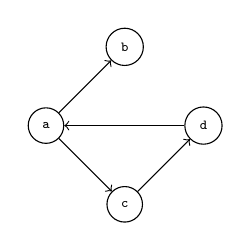
\begin{tikzpicture}
\node[draw, circle] (b) at (0, 0) {\tiny \texttt{b}};
\node[draw, circle] (a) at (-1, -1) {\tiny \texttt{a}};
\node[draw, circle] (d) at (1, -1) {\tiny \texttt{d}};
\node[draw, circle] (c) at (0, -2) {\tiny \texttt{c}};
\draw[->] (a) -- (b);
\draw[->] (a) -- (c);
\draw[->] (c) -- (d);
\draw[->] (d) -- (a);
\end{tikzpicture}
\end{center}
est repr\'{e}sent\'{e} par: \\

\noindent \texttt{link(a, b)}. \\
\texttt{link(a, c)}. \\
\texttt{link(c, d)}. \\
\texttt{link(d, a)}.

\begin{enumerate}
 \item \'{E}crivez un pr\'{e}dicat \texttt{path(X, Y)} qui est vrai s'il exsite un chemin de X \`{a} Y.
 \item Est-ce que l'ordre des pr\'{e}dicats dans votre programme a de l'importance?
 \item Comment calculer le chemin, et pas juste savoir s'il y en a un? Vous pouvez calculer le
 chemin dans l'ordre inverse si c'est plus simple.
 \item Comment on fait pour calculer tous les chemins entre X et Y?
\end{enumerate}

    \subsubsection*{Solution}
    \begin{enumerate}
    \item \textbf{TODO}
    \item \textbf{TODO}
    \item
    \begin{lstlisting}

    /* Partie 1 : Existence */

    link(a, b).
    link(a, c).
    link(c, d).
    link(d, a).

    path(X, Y) :- link(X, Y).
    path(X, Y) :- link(X, Z), path(Z, Y).

    /* Partie 2 : Ordre *

    path(X,Y) :- path(Z, Y), link(X, Z).
    %*\text{\% Fonctionne aussi, mais moins efficace.}*)
    %*\text{\% L’ordre des predicats n’a de l’importance que pour les performances.} *)

    /* Partie 3 : Chemin */

    link(a, b, [a, b]).
    link(a, c, [a, c]).
    link(c, d, [c, d]).

    path(X, Z, P) :- link(X, Z, P).
    path(X, Z, [X|P2]) :- link(X, Y, P1), path(Y, Z, P2).
    \end{lstlisting}

    \item Pour calculer tous les chemins, il suffit de lancer le programme de la partie 3, puis d'attendre une réponse.
    Lorsqu'on a une solution, on peut demander au programme de revenir en arrière et de modifier son dernier choix pour trouver une solution différente.
    En pratique, cela peut se faire en répondant à la réponse du programme par un ";" au lieu d'un ".".
    Il n'y a qu'à réitérer l'opération jusqu'à ce que le programme n'ait plus de choix disponible et qu'il se termine pour de bon.

   \end{enumerate}
\subsection*{Exercice 6}
Le programme suivant d\'{e}cide si un nombre est premier ou pas.

\begin{verbatim}
isPrime(2).
isPrime(3).
isPrime(P) :- P > 3, P mod 2 =\= 0, \+ hasFactor(P,3).
hasFactor(N,L) :- N mod L =:= 0.
hasFactor(N,L) :- L * L < N, L2 is L + 2, hasFactor(N,L2).
\end{verbatim}
Montrez les \'{e}tapes que prolog fait pour r\'{e}pondre aux requ\^{e}tes \texttt{isPrime(15)} et \texttt{isPrime(17)}.

    \subsubsection*{Solution}

    \begin{lstlisting}
    /* Requête initiale */
    r0 = < isPrime(15). >


    /* Résolution 1 */
    s1 = {(P, 15)}        % On sait que la variable P
                          % de la fonction isPrime vaut 15
    r1 = < 15>3, 15 mod 2 =\= 0, \+ hasFactor(15, 3). >
    % On developpe la fonction isPrime

    /* Résolution 2 */
    s2 = s1
    r2 = < 15 mod 2 =\= 0, \+ hasFactor(15, 3). >
    %15 est bien strictement superieur a 3

    /* Résolution 3 */
    s3 = s2
    r3 = < \+ hasFactor(15, 3). >
    %15 n'est pas divisible par 2

    /* Résolution 4 */
    s4 = s3 U {(L, 3)}     %On developpe hasFactor
    r4 = < \+ 3*3 < 15, L2 is 3+2, hasFactor(15, L2). >

    /* Résolution 5 */
    s5 = s4
    r5 = < \+ L2 is 3+2, hasFactor(15, L2). >

    /* Résolution 6 */
    s6 = s5 U {(L2, 5)}
    r6 = < \+ hasFactor(15, 5). >

    /* Résolution 7 */
    s7 = s6
    r7 = < \+ 15 mod 5 =:= 0. >
    %On passe dans le cas de base

    /* Résolution 8 */
    s8 = s7
    r8 = < \+ true >

    %La resolvante s'arrete car on a \+ true
    %(\+ implique que ce qui suit doit etre false)
    \end{lstlisting}

    \begin{lstlisting}
    /* Requête initiale */
    r0 = < isPrime(17). >


    /* Résolution 1 */
    s1 = {(P, 17)}        % Meme debut
    r1 = < 17>3, 17 mod 2 =\= 0, \+ hasFactor(17, 3). >

    /* Résolution 2 */
    s2 = s1
    r2 = < 17 mod 2 =\= 0, \+ hasFactor(17, 3). >

    /* Résolution 3 */
    s3 = s2
    r3 = < \+ hasFactor(17, 3). >

    /* Résolution 4 */
    s4 = s3 U {(L, 3)}     %On developpe hasFactor
    r4 = < \+ 3*3 < 17, L2 is 3+2, hasFactor(17, L2). >

    /* Résolution 5 */
    s5 = s4
    r5 = < \+ L2 is 3+2, hasFactor(17, L2). >

    /* Résolution 6 */
    s6 = s5 U {(L2, 5)}
    r6 = < \+ hasFactor(17, 5). >

    /* Résolution 7 */
    s7 = s6
    r7 = < \+ 5*5 < 17, L2' is 5+2, hasFactor(17, L2'). >
    %25 n'est pas inferieur a 17; false

    /* Résolution 8 */
    s8 = s7
    r8 = < \+ false >

    /* Résolution 9 */
    s9 = s8
    r9 = < >
    %La resolvante est vide
    %La requete renvoie true
    \end{lstlisting}


\section{TP 9}


\subsection*{Exercice 1}
Soient $x, y$ et $z$ trois n\oe{}uds distincts. On dit que $x$ est un \emph{n\oe{}ud pivot} pour $y$ et $z$ si tous les chemins les plus courts entre $y$ et $z$ passent par $x$.

\begin{enumerate}
\item Donnez un exemple d'un graphe o\`{u} tous les n\oe{}uds sont un n\oe{}ud pivot pour au moins une paire de n\oe{}uds.
\item Donnez un exemple d'un graphe o\`{u} tous les n\oe{}uds sont un n\oe{}ud pivot pour au moins trois paires de n\oe{}uds.
\item Soit $G$ un graphe qui repr\'{e}sente les liens d'amiti\'{e} d'un groupe de personnes. Si on suppose que la probabilit\'{e}e que deux personnes qui ne sont pas amies au 
temps $t$ deviennent amies au temps $t + 1$ est inversement proportionelle a la distance entre elles, quel est l'effet sur la probabilit\'{e} de retirer un personne pivot du graphe? 
\item Montrez qui si tous les n\oe{}uds sont un n\oe{}ud pivot pour au moins une paire de n\oe{}uds alors le graphe poss\'{e}de au moins un cycle.
\end{enumerate}

\subsubsection*{Solution}

\begin{enumerate}
	\item On prend $G = $
\begin{center}  
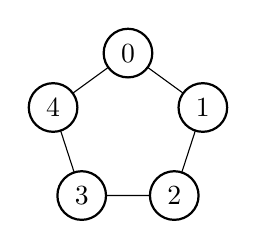
\begin{tikzpicture}
\tikzstyle{node}=[circle,draw,thick,fill=white]
\draw (90:1) node[node]{0}
-- (162:1) node[node]{4}
-- (234:1) node[node]{3}
-- (306:1) node[node]{2}
-- (378:1) node[node]{1}
-- cycle;
\end{tikzpicture}
\end{center}
$\forall i$ le noeud $i$ est pivot de $(i-1)\&(i+1)$ (modulo 5).

	\item On prend $G = $
\begin{center}  
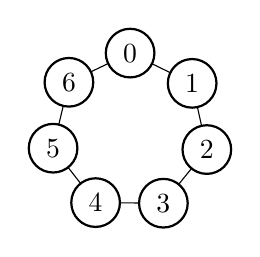
\begin{tikzpicture}
\tikzstyle{node}=[circle,draw,thick,fill=white]
\draw (90:1) node[node]{0}
-- (141:1) node[node]{6}
-- (192:1) node[node]{5}
-- (244:1) node[node]{4}
-- (295:1) node[node]{3}
-- (347:1) node[node]{2}
-- (398:1) node[node]{1}
-- cycle;
\end{tikzpicture}
\end{center}

$\forall i$ le noeud $i$ est pivot de : 
$(i-1) \& (i+1)$, $(i-1) \& (i+2)$ et $(i-2) \& (i+1)$ 
(modulo 7).
	\item Retirer le noeud pivot augmente la distance entre 2 personnes. Donc la probabilité que celles ci deviennent amies au temps $t+1$ diminue.

	\item On prouve d'abord que si un graphe n'a pas de cycle alors il possède au moins un noeud de degré 1.

Supposons que $G$ n'a pas de cycle et $V$ l'ensemble fini de ses noeuds.
Soit $x \in V$. On construit une séquence $P = (x_1, x_2, x_3, ...)$. Pour choisir $x_i (i>1)$, on prend un voisin de $x_{i-1}$ qiu n'a pas encore été choisi. Comme $V$ est fini, ce processus doit finir et on obtient $P= (x_1, x_2, x_3,...,x_k)$. 
Le noeud $k$ a un degré 1 car sinon il a un voisin $y\neq x_{k-1}$. Si $y \in P$ : Contradiction.
Si $y \notin P$, $x_k$ n'est pas la fin de la séquance : Contradiction.

On prouve ensuite que un noeud de degré un ne peu pas etre pivot.

Soit $x\in V$ tel que deg$(x)=1$.
Par hypothèse $x$ est pivot d'une paire $(y,z)$.
Donc il existe un chemin le plus court entre $y$ et $z$ qui passe bien par $x$.
Soit $w$ le seul voisin de $x$.
Mais alors il existe un chemin encore plus court : $(y, ..., w,...,z)$ qui ne passe pas par $x$.

% Insérer graphe 

\end{enumerate}
\subsection*{Exercice 2}
Soient $x, y$ et $z$ trois n\oe{}uds distincts. On dit que $x$ est un \emph{gardien} de $y$ et $z$ si tous les chemins entre $y$ et $z$ passent par $x$.
On dit qu'un n\oe{}ud $x$ est un \emph{gardien locale} s'il existent deux voisins de $x$ qui ne sont pas connect\'{e}s directement.
 
\begin{enumerate}
\item Donnez un exemple d'un graphe o\`{u} au moins la moiti\'{e} des n\oe{}uds sont
gardiens.
\item Donnez un exemple d'un graphe o\`{u} il n'y a pas de gardiens mais chaque n\oe{}ud est un gardien locale.
\item Quel est l'impacte sur un graphe de retirer un gardien?
\end{enumerate}

\subsubsection*{Solution}
\begin{enumerate}
	\item Les noeuds 1 et 2 sont gardien entre 0 et 3 

\begin{center}  
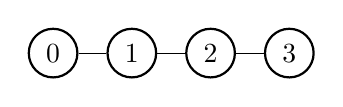
\begin{tikzpicture}
    \tikzstyle{node}=[circle,draw,thick,fill=white]
    \node[node] (0) at (0,0) {0};
    \node[node] (1) at (1,0) {1};
    \node[node] (2) at (2,0) {2};
    \node[node] (3) at (3,0) {3};

    \draw (0) -- (1);
    \draw (1) -- (2);
    \draw (2) -- (3);
\end{tikzpicture}
\end{center}

	\item  \hspace{1em}
	\vspace{1em}

\begin{center}  
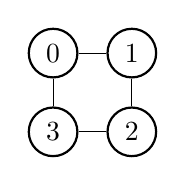
\begin{tikzpicture}
\tikzstyle{node}=[circle,draw,thick,fill=white]
    \node[node] (0) at (0,0) {0};
    \node[node] (1) at (1,0) {1};
    \node[node] (2) at (1,-1) {2};
    \node[node] (3) at (0,-1) {3};

    \draw (0) -- (1);
    \draw (1) -- (2);
    \draw (2) -- (3);
    \draw (3) -- (0);
\end{tikzpicture}
\end{center}

	\item Le graphe n'est plus connexe
\end{enumerate}

\subsection*{Exercice 3}

\begin{enumerate}
 \item Comment peut-on faire pour calculer efficacement les distances d'un n\oe{}uds a tout les autres?
 \item Un graphe est biparti si on peut s\'{e}parer les n\oe{}uds en deux ensembles $V_1$ et $V_2$ tells que
 $V_1 \cap V_2 = \emptyset$, $V_1 \cup V_2 = V$ et il n'y a pas d'ar\^{e}tes entre aucune paire de n\oe{}uds de $V_1$ et
 pas d'ar\^{e}tes entre aucune paire de n\oe{}uds de $V_2$. Soit $G$ un graphe connexe et $d_0(x)$ la distance du n\oe{}ud
 $0$ au n\oe{}ud $x$. Comment peut-on v\'{e}rifier que $G$ est bipartit a partir de $d_0$?
\end{enumerate}

\subsubsection*{Solution}
\begin{enumerate}

	\item On utilise l'algorithme BFS qui utilise une \texttt{Queue FIFO}
\begin{enumerate}
    \item Mettre le n\oe{}ud dans la Queue.
    \item Retirer le n\oe{}ud du début de la Queue pour l'examiner.
    \item Mettre tous les voisins non explorés dans la Queue.
    \item Si la file n'est pas vide reprendre à l'étape 2.
\end{enumerate}

Exemple : 

\begin{tabular}{lll}
    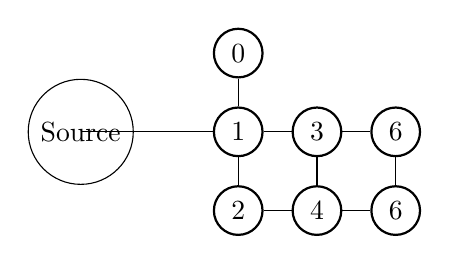
\begin{tikzpicture}
    \tikzstyle{node}=[circle,draw,thick,fill=white]
    \node[node] (2) at (0,0) {2};
    \node[node] (1) at (0,1) {1};
    \node[node] (0) at (0,2) {0};
    \node[node] (4) at (1,0) {4};
    \node[node] (3) at (1,1) {3};
    \node[node] (5) at (2,1) {6};
    \node[node] (6) at (2,0) {6};
    \node[] (S) at (-2,1) {Source};
    
    \draw (S) |- (1.west);
    \draw (0) -- (1);
    \draw (1) -- (2);
    \draw (3) -- (1);
    \draw (2) -- (4);
    \draw (4) -- (3);
    \draw (3) -- (5);
    \draw (6) -- (4);
    \draw (5) -- (6);
\end{tikzpicture}
&
  
&
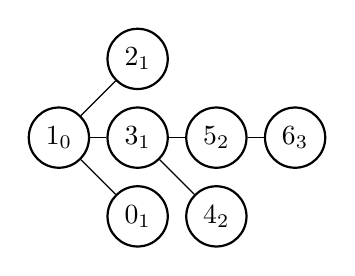
\begin{tikzpicture}
    \tikzstyle{node}=[circle,draw,thick,fill=white]
    \node[node] (1) at (0,1) {$1_{0}$};
    \node[node] (0) at (1,0) {$0_{1}$};
    \node[node] (3) at (1,1) {$3_{1}$};
    \node[node] (2) at (1,2) {$2_{1}$};
    \node[node] (5) at (2,1) {$5_{2}$};
    \node[node] (4) at (2,0) {$4_{2}$};
    \node[node] (6) at (3,1) {$6_{3}$};
    
    \draw (1) -- (0);
    \draw (1) -- (3);
    \draw (1) -- (2);
    \draw (3) -- (5);
    \draw (3) -- (4);
    \draw (5) -- (6);
\end{tikzpicture}
\end{tabular}

\item On vérifie qu'il n'existe pas d'arètes $(x,y)$ tel que $d_0(x)$ et $d_0(y)$ ont la meme parité

\end{enumerate}

% \vspace{0.5cm}
% 
% \subsection*{Exercice }
% Soient $x, y$ et $z$ trois n\oe{}uds distincts. On dit que $x$ est un \emph{gardien} de $y$ et $z$ si tous les chemins entre $y$ et $z$ passent par $x$.
% On dit qu'un n\oe{}ud $x$ est un \emph{gardien locale} s'il existent deux voisins de $x$ qui ne sont pas connect\'{e}s directement.
% 
% \begin{enumerate}
% \item Donnez un exemple d'un graphe o\`{u} au moins la moiti\'{e} des n\oe{}uds sont
% gardiens.
% \item Donnez un exemple d'un graphe o\`{u} il n'y a pas de gardiens mais chaque n\oe{}ud est un gardien locale.
% \end{enumerate}
% 

\subsection*{Exercice 4}
Le \emph{diam\`{e}tre} d'un graphe connexe est la distance maximum entre toutes les paires de n\oe{}uds. 
La \emph{distance moyenne} d'un graphe connexe c'est la moyenne des distances entre toutes les paires de n\oe{}uds. Formellement
$$
diam(G) = \max_{u, v} d(u, v)
$$
et
$$
l_G = \frac{1}{V (V - 1)} \sum_{u \neq v} d(u, v)
$$
o\'{u} $V$ est le nombre de n\oe{}uds de $G$.
\begin{enumerate}
\item Calculez le diam\`{e}tre et la distance moyenne du graphe $G_n$ suivant:
\begin{center}
\begin{tikzpicture}
\node[draw, circle] (A) at (0, 0) {0};
\node[draw, circle] (B) at (2, 0) {1};
\node[draw, circle] (C) at (4, 0) {2};
\node[draw, circle] (D) at (6, 0) {3};
\draw (A) -- (B) -- (C) -- (D);
\draw[dashed] (7, 0) circle (2);
\node at (9.5, 1) {$K_n$};
\draw (D) -- (7, 1);
\node at (7, 0.4) {$\vdots$};
\draw (D) -- (7, -0.5);
\draw (D) -- (7, -1);
\end{tikzpicture}
\end{center}
o\`{u} $K_n$ est le graphe complet avec $n$ n\oe{}uds. Par example, $G_4$ est le graphe:
\begin{center}
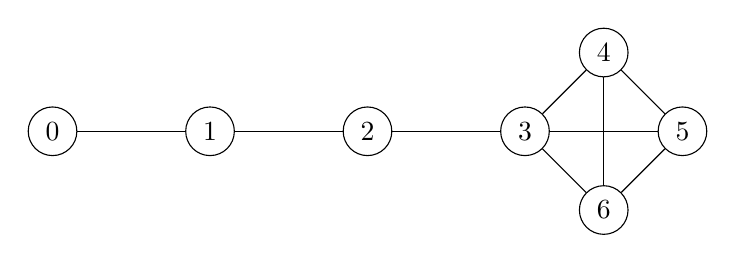
\begin{tikzpicture}
\node[draw, circle] (A) at (0, 0) {0};
\node[draw, circle] (B) at (2, 0) {1};
\node[draw, circle] (C) at (4, 0) {2};
\node[draw, circle] (D) at (6, 0) {3};
\node[draw, circle] (E) at (7, 1) {4};
\node[draw, circle] (F) at (8, 0) {5};
\node[draw, circle] (G) at (7, -1) {6};

\draw (A) -- (B) -- (C) -- (D);
\draw (D) -- (E);
\draw (D) -- (F);
\draw (D) -- (G);
\draw (E) -- (F);
\draw (E) -- (G);
\draw (G) -- (F);
\end{tikzpicture}
\end{center}


\item Montrez qu'il existe un graphe $G$ avec plus de $7$ n\oe{}uds tel que 
$$\frac{diam(G)}{l_G} = 2$$

\end{enumerate}


% \subsection*{Exercice }
% Calculez le coefficient regroupement de A et de B dans le graphe suivant:
% \begin{center}
% \begin{tikzpicture}
% \node[draw, circle] (A) at (0, 0)   {A};
% \node[draw, circle] (B) at (-2, 1)  {B};
% \node[draw, circle] (C) at (2, 1)   {C};
% \node[draw, circle] (D) at (2, -1)  {D};
% \node[draw, circle] (E) at (-2, -1) {E};
% \node[draw, circle] (F) at (-4, 0)  {F};
% \draw (A) -- (B);
% \draw (A) -- (C) -- (D);
% \draw (A) -- (D);
% \draw (A) -- (E) -- (B);
% \draw (B) -- (F) -- (E);
% \end{tikzpicture}
% \end{center}
% 
% 
% \vspace{0.5cm}

\subsubsection*{Solution}
\begin{enumerate}

	\item dim$(G) = 4$

Selon la table des distance:

\begin{tabular}{c|ccccc}
    &0&1&2&3& >3 \\
    \hline
    0 & 0& 1& 2& 3& 4\\
    1 & 1& 0&1& 2& 3\\
    2 & 2& 1& 0& 1&2\\
    3 & 1& 2& 3& 0&1\\
    >3 & 4& 3& 2& 1& 1 (0 si lui meme)\\
\end{tabular}

On peut calculer $\sum_{u\neq v} d(u,v)$.

\begin{align*}
    \sum_{u\neq v} d(u,v) =& 6 + 4(n-1)\\
    &+ 4 + 3(n-1)\\
    &+4+2(n-1)\\
    &+6+(n-1)\\
    &+(n-1)(10 + (n-2))\\
    =& 20 + (n-1)(4+3+2+1) + (n-1)(9 + (n-2))\\
    =& 20 + 10(n-1) + 9(n-1) + (n-1)^2\\
    =& 20 + 19(n-1) + (n-1)^2\\
    & \Rightarrow l_G (n) = \dfrac{n^2 + 17n + 2}{n^2 + 5n + 6}
\end{align*}


	\item $\dfrac{\text{diam}(G)}{l_G} = \dfrac{4}{l_G} =2$
\begin{align*}
    & \dfrac{4n^2 + 20n + 24}{n^2 + 17n + 2} = 2\\
    & \Rightarrow 4n^2 + 20n + 24 = 2n^2 + 34n + 4\\
    & \Rightarrow 2n^2 - 14n + 2\\
    & \Rightarrow n = 5\hspace{1em}\&\hspace{1em} n = 2\\
\end{align*}

Or $G$ doit comporter au moins 7 noeuds donc $G(5)$.

\end{enumerate}

\subsection*{Exercice 5}
On suppose qu'on est dans une communaut\'{e} ou les amiti\'{e}s sont repr\'{e}sent\'{e}es par un graphe $G$ connexe avec $n$ n\oe{}uds. 
Si chaque jour les amis des amis se rencontrent et deviennent amis, on s'interesse au nombre de jours $T(G)$ n\'{e}cessaires
pour que tout le monde deviennent ami, c'est-\`{a}-dire, pour le graphe deviennent $K_n$ (un graphe complet).
\begin{enumerate}
\item Supposons que $G = P_n$ (le chemin avec $n$ n\oe{}uds) et $T(P_n)$.
\item M\^{e}me question pour $G = C_n$ (le cycle avec $n$ n\oe{}uds).
\item Quel est la valeur de $T(G)$ en g\'{e}neral?
\end{enumerate}

\subsubsection*{Solution}
\begin{enumerate}

	\item Soit $A(i)$, les amis de $0$ au jour $i$.
\begin{align*}
    A(0) =& \{1 \} \\
    A(1) =& \{1,2 \}\\
    A(2) =& \{1,2,3,4 \}\\
    A(3) =& \{1,2,3,4,5,6,7,8, \}\\
    A(i) =& \{x+y | x,y \in A(i-1) \} \\
         =& \{1,2,3,..., 2^i \} \\
    T(P_n) =& \lceil \log_2 (n) \rceil
\end{align*}


	\item Le noeud le plus loin de $0$ dans un cycle de $n$ noeuds, est le noeud $\left\lfloor \dfrac{n}{2} \right\rfloor$
$$ T(C_n) = \left\lceil \log_2 \left(\left\lfloor \dfrac{n}{2} \right\rfloor \right) \right\rceil $$

	\item En général les noeuds à distance maximum prennent le plus de temps. Cette distance est le diamètre du graphe. Donc : 
$$ T(G) = \left\lceil \log_2 \left( \text{dim}(G) \right) \right\rceil $$


\end{enumerate}
% 
% \subsection*{Exercice }
% Calculez le coefficient de regroupement d'un n\oe{}ud de $C_n$, o\`{u} $n \geq 3$. Calculez le coefficient de regroupement de ce n\oe{}ud ap\`{e}s avoir ajout\'{e} les ar\^{e}tes entre les amis des amis dans le graphe. Commentez.
% 
% 
% 
% \subsection*{Exercice }
% \'{E}noncez la propri\'{e}t\'{e} de fermeture triadique forte. Est-ce que le graphe suivant poss\`{e}de cette propri\'{e}t\'{e}?
% 
% \begin{center}
% \begin{tikzpicture}
% \node[draw, circle] (A) at (0, 0) {A};
% \node[draw, circle] (B) at (2, 0) {B};
% \node[draw, circle] (C) at (0, -2) {C};
% \node[draw, circle] (D) at (-2, 0) {D};
% \node[draw, circle] (E) at (0, -4) {E};
% \node[draw, circle] (F) at (2, -2) {F};
% \node[draw, circle] (G) at (-2, -4) {G};
% \draw (G) -- (D) -- (A) -- (C) -- (F);
% \draw (C) -- (E);
% \draw[dashed] (G) -- (A) -- (B) -- (F) -- (E) -- (G);
% \draw[dashed] (D) -- (C);
% 
% \draw (4, -1) -- (5, -1) node[anchor = west] {lien fort};
% \draw[dashed] (4, -2) -- (5, -2) node[anchor = west] {lien faible};
% \end{tikzpicture}
% \end{center}
% 
% Supposons qu'un graphe poss\`{e}de la propri\'{e}t\'{e} de fermeture triadique forte. Si un lien faible devient fort, est-ce que cette propri\'{e}t\'{e} se maintien toujours? Et si un lien fort devient faible?
% 
% 

\section{TP 10}
%\addcontentsline{toc}{section}{TP 10}


\subsection*{Exercice 1}
Soit $G = (P, F)$ un graphe d'affiliations ($P$ rep\'{e}sente les personnes et $F$ les focus). On d\'{e}finit le \emph{graphe projet\'{e} sur les personnes} comme \'{e}tant un graphe avec ensemble de sommets $P$ et tel qu'il existe un lien entre deux personnes s'il existe un focus commun aux deux personnes dans $G$. \\

On consid\`{e}re le graphe d'affiliations suivant.
\begin{center}
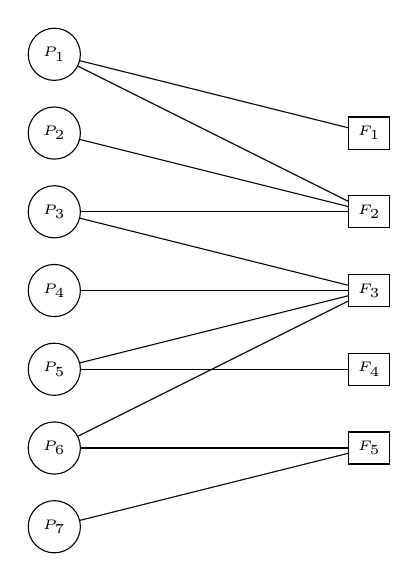
\begin{tikzpicture}
\node[draw, circle] at (0, 0) (P1) {\tiny $P_1$};
\node[draw, circle] at (0, -1) (P2) {\tiny $P_2$};
\node[draw, circle] at (0, -2) (P3) {\tiny $P_3$};
\node[draw, circle] at (0, -3) (P4) {\tiny $P_4$};
\node[draw, circle] at (0, -4) (P5) {\tiny $P_5$};
\node[draw, circle] at (0, -5) (P6) {\tiny $P_6$};
\node[draw, circle] at (0, -6) (P7) {\tiny $P_7$};
\node[draw, rectangle] at (4, -1) (F1) {\tiny $F_1$};
\node[draw, rectangle] at (4, -2) (F2) {\tiny $F_2$};
\node[draw, rectangle] at (4, -3) (F3) {\tiny $F_3$};
\node[draw, rectangle] at (4, -4) (F4) {\tiny $F_4$};
\node[draw, rectangle] at (4, -5) (F5) {\tiny $F_5$};
\draw (P1) -- (F1);
\draw (P1) -- (F2);
\draw (P2) -- (F2);
\draw (P3) -- (F2);
\draw (P3) -- (F3);
\draw (P4) -- (F3);
\draw (P5) -- (F3);
\draw (P5) -- (F4);
\draw (P6) -- (F3);
\draw (P6) -- (F5);
\draw (P7) -- (F5);
\end{tikzpicture}
\end{center}

\begin{enumerate}
\item Calculez le graphe projet\'{e} sur les personnes.

\item Donnez, si possible, un autre graphe d'affiliations avec la m\^{e}me projection sur les personnes.
\end{enumerate}

    \subsubsection*{Solution}
    La projection sur les personnes donne le graphe suivant :
    
    \begin{center}    
    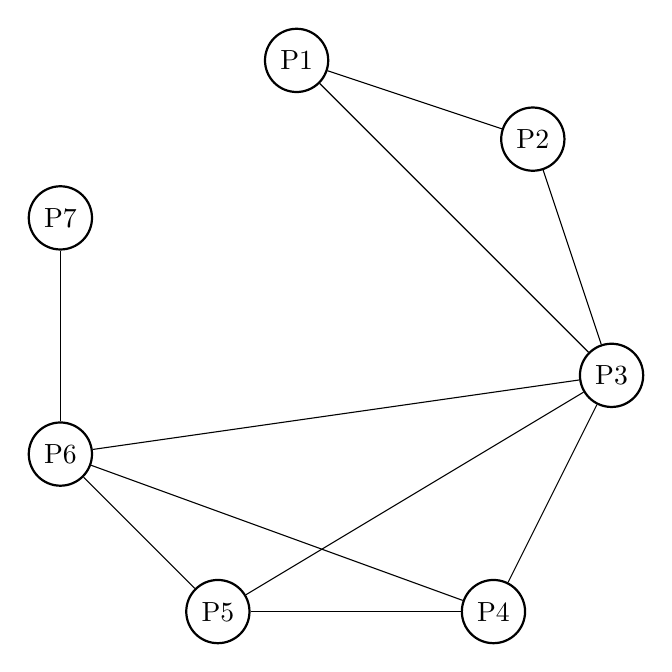
\begin{tikzpicture}
    \tikzstyle{node}=[circle,draw,thick,fill=white]
    \node[node] (P1) at (0,0) {P1};
    \node[node] (P2) at (3,-1) {P2};
    \node[node] (P3) at (4,-4) {P3};
    \node[node] (P4) at (2.5,-7) {P4};
    \node[node] (P5) at (-1,-7) {P5};
    \node[node] (P6) at (-3,-5) {P6};
    \node[node] (P7) at (-3,-2) {P7};
    \draw (P1) -- (P2);
    \draw (P1) -- (P3);
    \draw (P2) -- (P3);
    \draw (P3) -- (P4);
    \draw (P3) -- (P5);
    \draw (P3) -- (P6);
    \draw (P4) -- (P5);
    \draw (P4) -- (P6);
    \draw (P5) -- (P6);
    \draw (P6) -- (P7);
    \end{tikzpicture}
    \end{center}
    
    Il est facile d'obtenir la même projection avec un graphe d'affiliations différent.
    On peut pour cela rajouter un (ou plusieurs) focus relié(s) à une seule personne.
    Il est aussi possible de diviser un focus en 3 focus (vu plus en détail à la question 3).


\subsection*{Exercice 2}
\begin{enumerate}
\item
Calculez de graphe projet\'{e} sur les personnes du graphe d'affiliations suivant.
\begin{center}
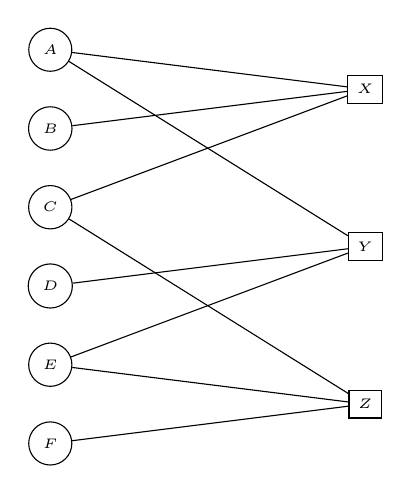
\begin{tikzpicture}
\node[draw, circle] at (0, 0) (A) {\tiny $A$};
\node[draw, circle] at (0, -1) (B) {\tiny $B$};
\node[draw, circle] at (0, -2) (C) {\tiny $C$};
\node[draw, circle] at (0, -3) (D) {\tiny $D$};
\node[draw, circle] at (0, -4) (E) {\tiny $E$};
\node[draw, circle] at (0, -5) (F) {\tiny $F$};
\node[draw, rectangle] at (4, -0.5) (X) {\tiny $X$};
\node[draw, rectangle] at (4, -2.5) (Y) {\tiny $Y$};
\node[draw, rectangle] at (4, -4.5) (Z) {\tiny $Z$};
\draw (A) -- (X);
\draw (A) -- (Y);
\draw (B) -- (X);
\draw (C) -- (X);
\draw (C) -- (Z);
\draw (D) -- (Y);
\draw (E) -- (Y);
\draw (E) -- (Z);
\draw (F) -- (Z);
\end{tikzpicture}
\end{center}
\item Dans le graphe r\'{e}sultant de la projection, expliquez la diff\`{e}rence qualitative entre le triangle $A$-$E$-$C$ et les autes.
\end{enumerate}

    \subsubsection*{Solution}
    Le graphe projeté sur les personnes est le suivant :
    
    \begin{center}    
    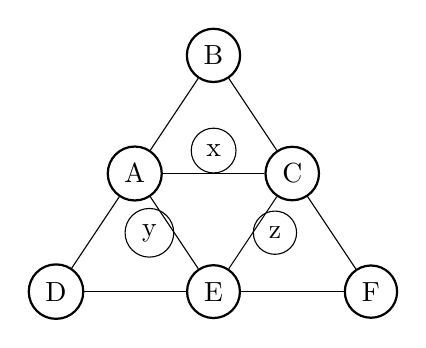
\begin{tikzpicture}
    \tikzstyle{node}=[circle,draw,thick,fill=white]
    \node[node] (A) at (1,1.5) {A};
    \node[node] (B) at (2,3) {B};
    \node[node] (C) at (3,1.5) {C};
    \node[node] (D) at (0,0) {D};
    \node[node] (E) at (2,0) {E};
    \node[node] (F) at (4,0) {F};
    \draw (A) -- (B);
    \draw (A) -- (C) node[midway,above]{x};
    \draw (A) -- (D);
    \draw (A) -- (E) node[midway,left]{y};
    \draw (B) -- (C);
    \draw (C) -- (E) node[midway,right]{z};
    \draw (C) -- (F);
    \draw (D) -- (E);
    \draw (E) -- (F);
    \end{tikzpicture}
    \end{center}
    
    La différence entre le triangle A-E-C et les autres est que celui-ci ne correspond pas à 1 seul et unique focus.
    En effet, A-C correspond à x, A-E à y, et C-E à z.\\
    Il y a d'ailleurs un théorème important qui signale que lorsque la projection sur les personnes contient un sous-graphe complet, cela n'implique pas l'existence d'un focus commun à tous ses noeuds.
    

\subsection*{Exercice 3}
Quel est le nombre minimum de focus qu'il faut avoir dans un graphe d'affiliation
pour que sa projection sur les personnes soit le graphe complet si il n'y a pas de focus commum \`{a} toutes les personnes?

    \subsubsection*{Solution}
    Il faut au minimum \textbf{trois} focus pour que la projection sur les personnes donne un graphe complet sans avoir de focus commun à tous.
    
    On prouve tout d'abord que cela ne fonctionne pas avec moins de 3 focus.\\
    Si l'on prend 1 seul focus, le seul moyen d'obtenir le graphe complet est de relier toutes les personnes à ce focus, et on aura donc 1 focus commun à tous.\\
    Si l'on prend 2 focus, on peut démarrer avec 3 personnes et voir qu'il est impossible d'obtenir $K_3$ avec la projection sur les personnes.
    En effet, pour éviter d'avoir un focus commun, on prend 2 de ces personnes et on les relie chacune à un focus différent.
    La $3^{\text{ème}}$ personne est reliée aux 2 focus, et donc aux 2 autres.
    Mais il est donc impossible de connecter les 2 premières sans que toutes aient un focus commun.\\
    On a donc montré qu'on ne pourra pas employer moins de 3 focus.
    
    Prouvons maintenant que 3 focus suffisent.\\
    On reprend le principe de la construction effectuée précédemment pour 2 focus et 3 personnes.
    On relie 2 personnes à 2 focus différents.
    Ensuite, on relie la $3^{\text{ème}}$ à ces 2 focus.
    Il ne reste qu'à connecter les 2 premières grâce au $3^{\text{ème}}$ focus inoccupé.
    Chaque focus n'est donc commun qu'à 2 personnes, et donc aucun n'est commun à toutes les personnes.\\
    Si l'on ajoute une personne, il ne faut le relier qu'à 2 focus pour le relier aux autres.
    On peut par exemple l'attacher aux mêmes focus que la $3^{\text{ème}}$ personne, de sorte qu'il soit connecté à toutes les autres.
    Le focus commun aux 2 premières reste uniquement lié à ces 2 personnes.
    On peut donc continuer à rajouter des personnes sans déroger à cette règle.\\
    On a donc montré que 3 focus suffisent à obtenir le résultat souhaité, ceci termine la preuve.
    

\subsection*{Exercice 4}
Dans une \'{e}tude sur trois petits villages $A, B$ et $C$ chacun habit\'{e} par 30 personnes, on a construit un r\'{e}seau social avec les personnes des trois villages et on a
constat\'{e} que chaque personne est amie avec les personnes du m\^{e}me village mais enemie des personnes des deux autres villages. 
\begin{enumerate}
\item Est-ce que le graph satisfait la propri\'{e}t\'{e} de balance structurelle? 
\item Et la prori\'{e}t\'{e} de balance structurelle faible?
\item Est-ce qu'il existent des triangles $(-,-,-)$? Et $(+,+,-)$?
\end{enumerate}

    \subsubsection*{Solution}
    \noindent \underline{Rappel} :\\
    Un graphe contenant $N$ n\oe{}uds, satisfait la propriété d'équilibre structurel si et seulement si il peut être séparé en deux parties telles que chaque partie contient uniquement des $+$, et qu'il n'y a que des $-$ entre ces deux parties, chaque partie contenant entre $0$ et $N$ n\oe{}uds.\\
    La propriété d'équilibre structurel faible correspond à un graphe qui peut être séparé en plus de deux parties qui respectent les conditions sus-mentionnées.

    Exemples de graphes équilibrés :
    \begin{center}    
    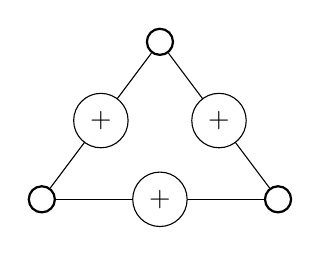
\begin{tikzpicture}
    \tikzstyle{node}=[circle,draw,thick,fill=white]
    \node[node] (A) at (0,0) {};
    \node[node] (B) at (1.5,-2) {};
    \node[node] (C) at (-1.5,-2) {};
    \draw (A) -- (B) node[midway,fill=white]{+};
    \draw (A) -- (C) node[midway,fill=white]{+};
    \draw (B) -- (C) node[midway,fill=white]{+};
    \end{tikzpicture}
    \hspace{2cm}
    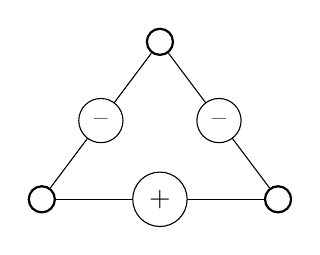
\begin{tikzpicture}
    \tikzstyle{node}=[circle,draw,thick,fill=white]
    \node[node] (A) at (0,0) {};
    \node[node] (B) at (1.5,-2) {};
    \node[node] (C) at (-1.5,-2) {};
    \draw (A) -- (B) node[midway,fill=white]{--};
    \draw (A) -- (C) node[midway,fill=white]{--};
    \draw (B) -- (C) node[midway,fill=white]{+};
    \end{tikzpicture}
    \end{center}
    
    Exemples de graphes faiblement équilibrés :
    \begin{center}    
    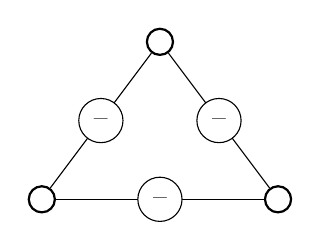
\begin{tikzpicture}
    \tikzstyle{node}=[circle,draw,thick,fill=white]
    \node[node] (A) at (0,0) {};
    \node[node] (B) at (1.5,-2) {};
    \node[node] (C) at (-1.5,-2) {};
    \draw (A) -- (B) node[midway,fill=white]{--};
    \draw (A) -- (C) node[midway,fill=white]{--};
    \draw (B) -- (C) node[midway,fill=white]{--};
    \end{tikzpicture}
    \hspace{2cm}
    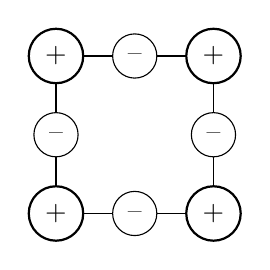
\begin{tikzpicture}
    \tikzstyle{node}=[circle,draw,thick,fill=white]
    \node[node] (A) at (0,0) {+};
    \node[node] (B) at (2,0) {+};
    \node[node] (C) at (2,-2) {+};
    \node[node] (D) at (0,-2) {+};
    \draw (A) -- (B) node[midway,fill=white]{--};
    \draw (A) -- (D) node[midway,fill=white]{--};
    \draw (B) -- (C) node[midway,fill=white]{--};
    \draw (C) -- (D) node[midway,fill=white]{--};
    \end{tikzpicture}
    \end{center}
    
    Exemple de graphe non équilibré :
    \begin{center}    
    \hspace{2cm}
    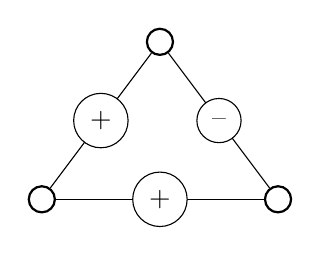
\begin{tikzpicture}
    \tikzstyle{node}=[circle,draw,thick,fill=white]
    \node[node] (A) at (0,0) {};
    \node[node] (B) at (1.5,-2) {};
    \node[node] (C) at (-1.5,-2) {};
    \draw (A) -- (B) node[midway,fill=white]{--};
    \draw (A) -- (C) node[midway,fill=white]{+};
    \draw (B) -- (C) node[midway,fill=white]{+};
    \end{tikzpicture}
    \end{center}
    
    \noindent \underline{Solution}:
    
    Le graphe de cette situation peut être représenté comme suit :
    \begin{center}    
    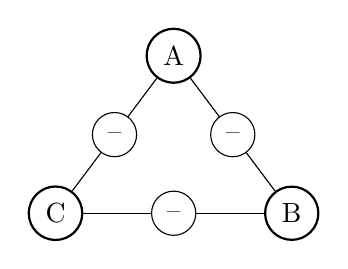
\begin{tikzpicture}
    \tikzstyle{node}=[circle,draw,thick,fill=white]
    \node[node] (A) at (0,0) {A};
    \node[node] (B) at (1.5,-2) {B};
    \node[node] (C) at (-1.5,-2) {C};
    \draw (A) -- (B) node[midway,fill=white]{--};
    \draw (A) -- (C) node[midway,fill=white]{--};
    \draw (B) -- (C) node[midway,fill=white]{--};
    \end{tikzpicture}
    \end{center}
    
    Avec les noeuds A, B et C tels qu'ils ne contiennent que des $+$.
    On peut donc le retracer :
    
    \begin{center}
    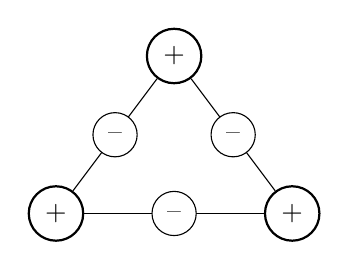
\begin{tikzpicture}
    \tikzstyle{node}=[circle,draw,thick,fill=white]
    \node[node] (A) at (0,0) {+};
    \node[node] (B) at (1.5,-2) {+};
    \node[node] (C) at (-1.5,-2) {+};
    \draw (A) -- (B) node[midway,fill=white]{--};
    \draw (A) -- (C) node[midway,fill=white]{--};
    \draw (B) -- (C) node[midway,fill=white]{--};
    \end{tikzpicture}
    \end{center}
    
    Ce graphe ne satisfait pas la propriété de balance structurelle.
    En revanche, il respecte l'équilibre faible.\\
    On constate qu'il existe des triangles ($-$, $-$, $-$) : il suffit de prendre 3 personnes issues de 3 villages différents.
    Il n'y a pas de triangles ($+$, $+$, $-$) : pour avoir un lien $-$, il faut prendre 2 personnes de 2 villages différents, et pour avoir un lien $+$ il faut 2 personnes du même village. D'autre part, la présence de tels triangles donnerait un graphe non-équilibré.


\subsection*{Exercice 5}
Soit $K_n$ le graphe complet avec $n \geq 5$ sommets. Supposons que les liens $(1, 2)$, $(2, 3)$, $(3, 4)$, $\ldots$ $(n - 1, n)$, $(n, 1)$ sont positifs et que tous les autres
liens sont n\'{e}gatifs. Pour chaque lien comptez le nombre de triangles balanc\'{e}s et non balanc\'{e}s auxquelles il appartient.

    \subsubsection*{Solution}
    Il y a deux types de triangles balancés :
    \begin{enumerate}
        \item Les triangles composés uniquement de liens positifs : ce graphe n'en compte aucun.
        \item Les triangles composés d'un seul lien positif et de deux liens négatifs : à chaque lien positif correspondent $n-4$ triangles de cette sorte (on retire les 2 noeuds incidents au lien, ainsi que les 2 noeuds qui leur sont adjacents par un lien positif).
    \end{enumerate}
    
    Il n'y a par contre qu'un seul type de triangle non-balancé contenant un lien positif : les triangles contenant deux liens positifs et un négatif.
    Pour chaque lien positif il y en a $2$ ("un de chaque côté").
    
    Puisqu'il y a $n$ lien positifs, il y a donc au total $n(n-4)$ triangles balancés. Il y a également $\dfrac{2n}{2}$ triangles non balancés pour ces liens positifs. On divise par deux, car chacun de ces triangles emploie 2 liens positifs.
    
    On peut vérifier tout cela en comptant le nombre total de triangles possédant un lien positif.
    Ce nombre est $n(n-2) - n = n(n-3)$. Le terme $(n-2)$ vient du fait qu'on compte ici les triangles en prenant les deux noeuds incidents à chaque lien positif. On doit ensuite en retirer $n$, sinon on compterait deux fois chaque triangle composé de deux liens positifs.
    On vérifie donc bien $n(n-4) + n = n(n-3)$, le compte est bon.

\subsection*{Exercice 6}
Si $G$ est complet et non \'{e}quilibr\'{e} est-ce possible d'introduire un nouveau sommet tel que tout les triangles auxquels ce sommet appartient soient \'{e}quilibr\'{e}s?
Si oui donnez une procedure pour le faire. Sinon donnez une preuve.

    \subsubsection*{Solution}
    Si G est complet et non équilibré il est impossible d’introduire un nouveau sommet tel que tous les triangles auxquels ce sommet appartient soient équilibrés en gardant le caractère complet de G.
    En revanche, si l'on ne conserve pas cette propriété, l'opération est possible.\\
    Si G ne possède que des liens négatifs, il suffit de relier un sommet au nouveau par un lien positif, et un autre sommet par un lien négatif.
    On obtiendra ainsi un (et un seul, il est impossible d'en créer plus) triangle ($+$, $-$, $-$), qui est équilibré.\\
    Si G possède des triangles du type ($+$, $+$, $-$), on peut relier le nouveau sommet à deux sommets liés par un lien négatif comme dans le cas précédent ($+$, $-$, $-$) ; ou à deux sommets liés par un lien positif avec deux liens positifs ($+$, $+$, $+$) ; ou à deux sommets liés par un lien positif avec un lien positif et un lien négatif ($+$, $-$, $-$).
    

\subsection*{Exercice 7}
Soit $G$ un triangle \'{e}quilibr\'{e}. De combien de fa\c{c}ons peut-on ajouter un sommet en gardant l'\'{e}quilibre structurel?

    \subsubsection*{Solution}
    Commençons par le premier type de triangles équilibrés :
    \begin{center}    
    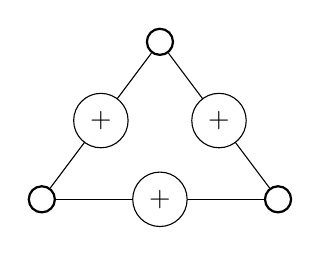
\begin{tikzpicture}
    \tikzstyle{node}=[circle,draw,thick,fill=white]
    \node[node] (A) at (0,0) {};
    \node[node] (B) at (1.5,-2) {};
    \node[node] (C) at (-1.5,-2) {};
    \draw (A) -- (B) node[midway,fill=white]{+};
    \draw (A) -- (C) node[midway,fill=white]{+};
    \draw (B) -- (C) node[midway,fill=white]{+};
    \end{tikzpicture}
    \end{center}
    
    \begin{center}    
    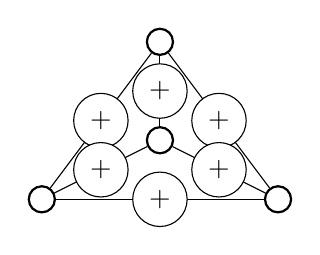
\begin{tikzpicture}
    \tikzstyle{node}=[circle,draw,thick,fill=white]
    \node[node] (A) at (0,0) {};
    \node[node] (B) at (1.5,-2) {};
    \node[node] (C) at (-1.5,-2) {};
    \node[node] (D) at (0,-1.25) {};
    \draw (A) -- (B) node[midway,fill=white]{+};
    \draw (A) -- (C) node[midway,fill=white]{+};
    \draw (B) -- (C) node[midway,fill=white]{+};
    \draw (D) -- (A) node[midway,fill=white]{+};
    \draw (D) -- (B) node[midway,fill=white]{+};
    \draw (D) -- (C) node[midway,fill=white]{+};
    \end{tikzpicture}
    \hspace{0.5cm}
    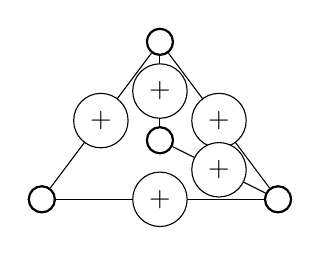
\begin{tikzpicture}
    \tikzstyle{node}=[circle,draw,thick,fill=white]
    \node[node] (A) at (0,0) {};
    \node[node] (B) at (1.5,-2) {};
    \node[node] (C) at (-1.5,-2) {};
    \node[node] (D) at (0,-1.25) {};
    \draw (A) -- (B) node[midway,fill=white]{+};
    \draw (A) -- (C) node[midway,fill=white]{+};
    \draw (B) -- (C) node[midway,fill=white]{+};
    \draw (D) -- (A) node[midway,fill=white]{+};
    \draw (D) -- (B) node[midway,fill=white]{+};
    \end{tikzpicture}
    \hspace{0.5cm}
    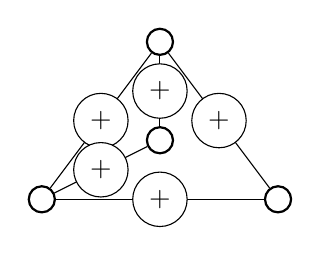
\begin{tikzpicture}
    \tikzstyle{node}=[circle,draw,thick,fill=white]
    \node[node] (A) at (0,0) {};
    \node[node] (B) at (1.5,-2) {};
    \node[node] (C) at (-1.5,-2) {};
    \node[node] (D) at (0,-1.25) {};
    \draw (A) -- (B) node[midway,fill=white]{+};
    \draw (A) -- (C) node[midway,fill=white]{+};
    \draw (B) -- (C) node[midway,fill=white]{+};
    \draw (D) -- (A) node[midway,fill=white]{+};
    \draw (D) -- (C) node[midway,fill=white]{+};
    \end{tikzpicture}
    \hspace{0.5cm}
    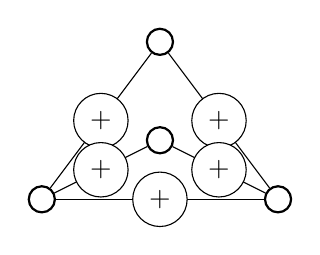
\begin{tikzpicture}
    \tikzstyle{node}=[circle,draw,thick,fill=white]
    \node[node] (A) at (0,0) {};
    \node[node] (B) at (1.5,-2) {};
    \node[node] (C) at (-1.5,-2) {};
    \node[node] (D) at (0,-1.25) {};
    \draw (A) -- (B) node[midway,fill=white]{+};
    \draw (A) -- (C) node[midway,fill=white]{+};
    \draw (B) -- (C) node[midway,fill=white]{+};
    \draw (D) -- (B) node[midway,fill=white]{+};
    \draw (D) -- (C) node[midway,fill=white]{+};
    \end{tikzpicture}
    
    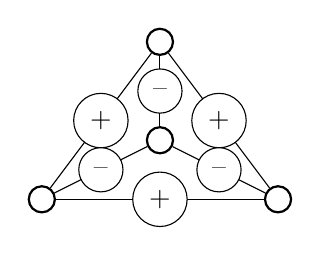
\begin{tikzpicture}
    \tikzstyle{node}=[circle,draw,thick,fill=white]
    \node[node] (A) at (0,0) {};
    \node[node] (B) at (1.5,-2) {};
    \node[node] (C) at (-1.5,-2) {};
    \node[node] (D) at (0,-1.25) {};
    \draw (A) -- (B) node[midway,fill=white]{+};
    \draw (A) -- (C) node[midway,fill=white]{+};
    \draw (B) -- (C) node[midway,fill=white]{+};
    \draw (D) -- (A) node[midway,fill=white]{--};
    \draw (D) -- (B) node[midway,fill=white]{--};
    \draw (D) -- (C) node[midway,fill=white]{--};
    \end{tikzpicture}
    \hspace{0.5cm}
    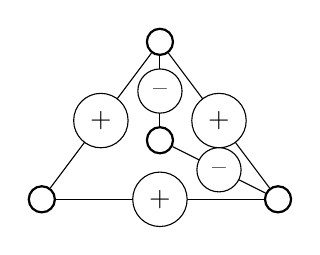
\begin{tikzpicture}
    \tikzstyle{node}=[circle,draw,thick,fill=white]
    \node[node] (A) at (0,0) {};
    \node[node] (B) at (1.5,-2) {};
    \node[node] (C) at (-1.5,-2) {};
    \node[node] (D) at (0,-1.25) {};
    \draw (A) -- (B) node[midway,fill=white]{+};
    \draw (A) -- (C) node[midway,fill=white]{+};
    \draw (B) -- (C) node[midway,fill=white]{+};
    \draw (D) -- (A) node[midway,fill=white]{--};
    \draw (D) -- (B) node[midway,fill=white]{--};
    \end{tikzpicture}
    \hspace{0.5cm}
    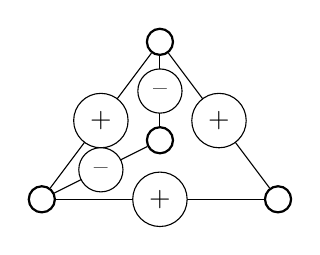
\begin{tikzpicture}
    \tikzstyle{node}=[circle,draw,thick,fill=white]
    \node[node] (A) at (0,0) {};
    \node[node] (B) at (1.5,-2) {};
    \node[node] (C) at (-1.5,-2) {};
    \node[node] (D) at (0,-1.25) {};
    \draw (A) -- (B) node[midway,fill=white]{+};
    \draw (A) -- (C) node[midway,fill=white]{+};
    \draw (B) -- (C) node[midway,fill=white]{+};
    \draw (D) -- (A) node[midway,fill=white]{--};
    \draw (D) -- (C) node[midway,fill=white]{--};
    \end{tikzpicture}
    \hspace{0.5cm}
    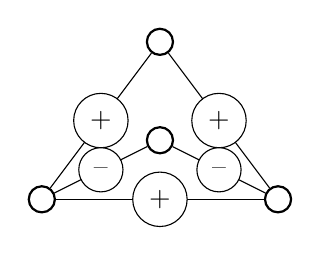
\begin{tikzpicture}
    \tikzstyle{node}=[circle,draw,thick,fill=white]
    \node[node] (A) at (0,0) {};
    \node[node] (B) at (1.5,-2) {};
    \node[node] (C) at (-1.5,-2) {};
    \node[node] (D) at (0,-1.25) {};
    \draw (A) -- (B) node[midway,fill=white]{+};
    \draw (A) -- (C) node[midway,fill=white]{+};
    \draw (B) -- (C) node[midway,fill=white]{+};
    \draw (D) -- (B) node[midway,fill=white]{--};
    \draw (D) -- (C) node[midway,fill=white]{--};
    \end{tikzpicture}
    \end{center}
    
    Pour le second type de triangles équilibrés :
    \begin{center}    
    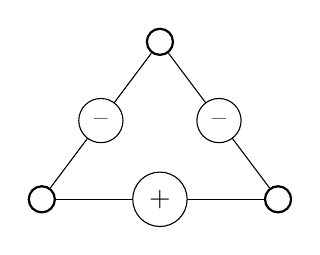
\begin{tikzpicture}
    \tikzstyle{node}=[circle,draw,thick,fill=white]
    \node[node] (A) at (0,0) {};
    \node[node] (B) at (1.5,-2) {};
    \node[node] (C) at (-1.5,-2) {};
    \draw (A) -- (B) node[midway,fill=white]{--};
    \draw (A) -- (C) node[midway,fill=white]{--};
    \draw (B) -- (C) node[midway,fill=white]{+};
    \end{tikzpicture}
    
    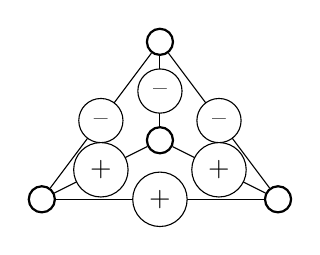
\begin{tikzpicture}
    \tikzstyle{node}=[circle,draw,thick,fill=white]
    \node[node] (A) at (0,0) {};
    \node[node] (B) at (1.5,-2) {};
    \node[node] (C) at (-1.5,-2) {};
    \node[node] (D) at (0,-1.25) {};
    \draw (A) -- (B) node[midway,fill=white]{--};
    \draw (A) -- (C) node[midway,fill=white]{--};
    \draw (B) -- (C) node[midway,fill=white]{+};
    \draw (D) -- (A) node[midway,fill=white]{--};
    \draw (D) -- (B) node[midway,fill=white]{+};
    \draw (D) -- (C) node[midway,fill=white]{+};
    \end{tikzpicture}
    \hspace{0.5cm}
    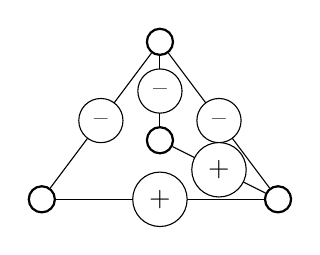
\begin{tikzpicture}
    \tikzstyle{node}=[circle,draw,thick,fill=white]
    \node[node] (A) at (0,0) {};
    \node[node] (B) at (1.5,-2) {};
    \node[node] (C) at (-1.5,-2) {};
    \node[node] (D) at (0,-1.25) {};
    \draw (A) -- (B) node[midway,fill=white]{--};
    \draw (A) -- (C) node[midway,fill=white]{--};
    \draw (B) -- (C) node[midway,fill=white]{+};
    \draw (D) -- (A) node[midway,fill=white]{--};
    \draw (D) -- (B) node[midway,fill=white]{+};
    \end{tikzpicture}
    \hspace{0.5cm}
    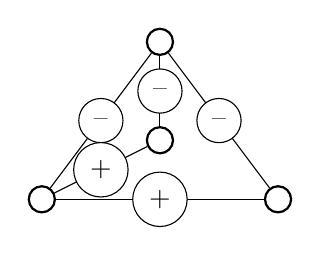
\begin{tikzpicture}
    \tikzstyle{node}=[circle,draw,thick,fill=white]
    \node[node] (A) at (0,0) {};
    \node[node] (B) at (1.5,-2) {};
    \node[node] (C) at (-1.5,-2) {};
    \node[node] (D) at (0,-1.25) {};
    \draw (A) -- (B) node[midway,fill=white]{--};
    \draw (A) -- (C) node[midway,fill=white]{--};
    \draw (B) -- (C) node[midway,fill=white]{+};
    \draw (D) -- (A) node[midway,fill=white]{--};
    \draw (D) -- (C) node[midway,fill=white]{+};
    \end{tikzpicture}
    \hspace{0.5cm}
    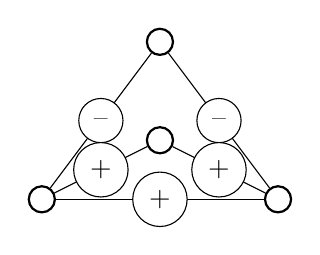
\begin{tikzpicture}
    \tikzstyle{node}=[circle,draw,thick,fill=white]
    \node[node] (A) at (0,0) {};
    \node[node] (B) at (1.5,-2) {};
    \node[node] (C) at (-1.5,-2) {};
    \node[node] (D) at (0,-1.25) {};
    \draw (A) -- (B) node[midway,fill=white]{--};
    \draw (A) -- (C) node[midway,fill=white]{--};
    \draw (B) -- (C) node[midway,fill=white]{+};
    \draw (D) -- (B) node[midway,fill=white]{+};
    \draw (D) -- (C) node[midway,fill=white]{+};
    \end{tikzpicture}
    
    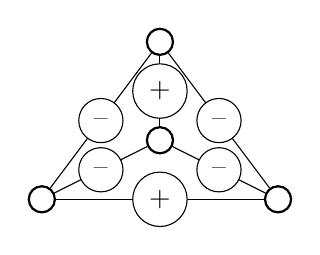
\begin{tikzpicture}
    \tikzstyle{node}=[circle,draw,thick,fill=white]
    \node[node] (A) at (0,0) {};
    \node[node] (B) at (1.5,-2) {};
    \node[node] (C) at (-1.5,-2) {};
    \node[node] (D) at (0,-1.25) {};
    \draw (A) -- (B) node[midway,fill=white]{--};
    \draw (A) -- (C) node[midway,fill=white]{--};
    \draw (B) -- (C) node[midway,fill=white]{+};
    \draw (D) -- (A) node[midway,fill=white]{+};
    \draw (D) -- (B) node[midway,fill=white]{--};
    \draw (D) -- (C) node[midway,fill=white]{--};
    \end{tikzpicture}
    \hspace{0.5cm}
    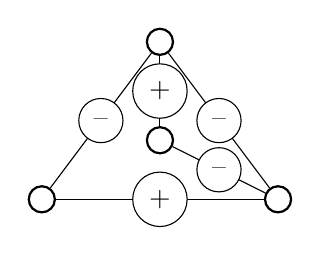
\begin{tikzpicture}
    \tikzstyle{node}=[circle,draw,thick,fill=white]
    \node[node] (A) at (0,0) {};
    \node[node] (B) at (1.5,-2) {};
    \node[node] (C) at (-1.5,-2) {};
    \node[node] (D) at (0,-1.25) {};
    \draw (A) -- (B) node[midway,fill=white]{--};
    \draw (A) -- (C) node[midway,fill=white]{--};
    \draw (B) -- (C) node[midway,fill=white]{+};
    \draw (D) -- (A) node[midway,fill=white]{+};
    \draw (D) -- (B) node[midway,fill=white]{--};
    \end{tikzpicture}
    \hspace{0.5cm}
    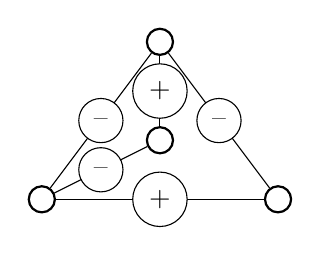
\begin{tikzpicture}
    \tikzstyle{node}=[circle,draw,thick,fill=white]
    \node[node] (A) at (0,0) {};
    \node[node] (B) at (1.5,-2) {};
    \node[node] (C) at (-1.5,-2) {};
    \node[node] (D) at (0,-1.25) {};
    \draw (A) -- (B) node[midway,fill=white]{--};
    \draw (A) -- (C) node[midway,fill=white]{--};
    \draw (B) -- (C) node[midway,fill=white]{+};
    \draw (D) -- (A) node[midway,fill=white]{+};
    \draw (D) -- (C) node[midway,fill=white]{--};
    \end{tikzpicture}
    \hspace{0.5cm}
    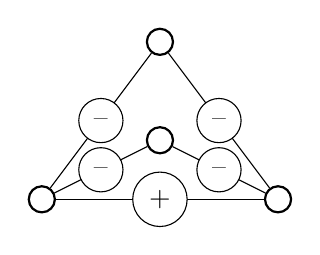
\begin{tikzpicture}
    \tikzstyle{node}=[circle,draw,thick,fill=white]
    \node[node] (A) at (0,0) {};
    \node[node] (B) at (1.5,-2) {};
    \node[node] (C) at (-1.5,-2) {};
    \node[node] (D) at (0,-1.25) {};
    \draw (A) -- (B) node[midway,fill=white]{--};
    \draw (A) -- (C) node[midway,fill=white]{--};
    \draw (B) -- (C) node[midway,fill=white]{+};
    \draw (D) -- (B) node[midway,fill=white]{--};
    \draw (D) -- (C) node[midway,fill=white]{--};
    \end{tikzpicture}
    \end{center}


\subsection*{Exercice 8}
Est-ce que les graphes suivants ont la propri\'{e}t\'{e} d'\'{e}quilibre structurel? Et d'\'{e}quilibre stucturel faible?
\begin{center}
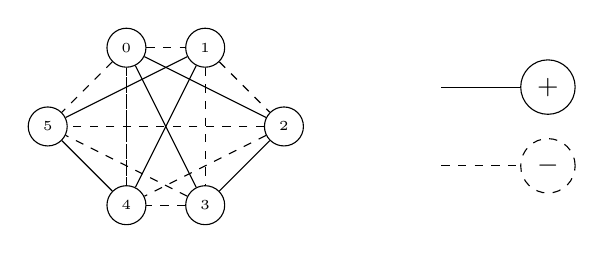
\begin{tikzpicture}
\node[draw, circle] at (0, 0) (a) {\tiny $0$};
\node[draw, circle] at (1, 0) (b) {\tiny $1$};
\node[draw, circle] at (2, -1) (c) {\tiny $2$};
\node[draw, circle] at (1, -2) (d) {\tiny $3$};
\node[draw, circle] at (0, -2) (e) {\tiny $4$};
\node[draw, circle] at (-1, -1) (f) {\tiny $5$};
%\draw (a) -- (0.5, -1) node[anchor=east] {\tiny $+$} -- (d);
%\draw (c) -- (1.5, -1.5) node[anchor=east] {\tiny $+$} -- (d);
%\draw (f) -- (0, -0.5) node {\tiny $+$} -- (b);
%\draw (b) -- (0.5, -1) node {\tiny $+$} -- (e);
\draw (a) -- (d) -- (c) -- (a);
\draw (f) -- (b) -- (e) -- (f);
\draw[dashed] (a) -- (b);
\draw[dashed] (a) -- (e);
\draw[dashed] (a) -- (f);
\draw[dashed] (b) -- (c);
\draw[dashed] (b) -- (d);
\draw[dashed] (c) -- (e);
\draw[dashed] (c) -- (f);
\draw[dashed] (d) -- (e);
\draw[dashed] (d) -- (f);
\draw[dashed] (e) -- (a);

\draw (4, -0.5) -- (5, -0.5) node[anchor = west] {$+$};
\draw[dashed] (4, -1.5) -- (5, -1.5) node[anchor = west] {$-$};
\end{tikzpicture}
\end{center}

\begin{center}
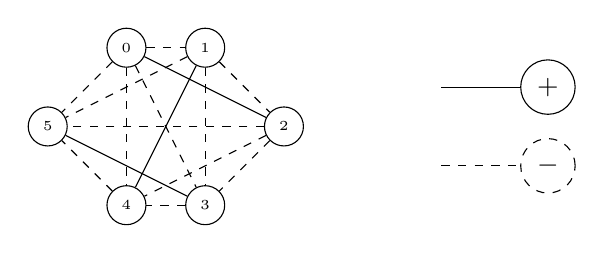
\begin{tikzpicture}
\node[draw, circle] at (0, 0) (a) {\tiny $0$};
\node[draw, circle] at (1, 0) (b) {\tiny $1$};
\node[draw, circle] at (2, -1) (c) {\tiny $2$};
\node[draw, circle] at (1, -2) (d) {\tiny $3$};
\node[draw, circle] at (0, -2) (e) {\tiny $4$};
\node[draw, circle] at (-1, -1) (f) {\tiny $5$};
%\draw (a) -- (0.5, -1) node[anchor=east] {\tiny $+$} -- (d);
%\draw (c) -- (1.5, -1.5) node[anchor=east] {\tiny $+$} -- (d);
%\draw (f) -- (0, -0.5) node {\tiny $+$} -- (b);
%\draw (b) -- (0.5, -1) node {\tiny $+$} -- (e);
\draw[dashed] (a) -- (b);
\draw[] (a) -- (c);
\draw[dashed] (a) -- (d);
\draw[dashed] (a) -- (e);
\draw[dashed] (a) -- (f);
\draw[dashed] (b) -- (c);
\draw[dashed] (b) -- (d);
\draw[] (b) -- (e);
\draw[dashed] (b) -- (f);
\draw[dashed] (c) -- (d);
\draw[dashed] (c) -- (e);
\draw[dashed] (c) -- (f);
\draw[dashed] (d) -- (e);
\draw[] (d) -- (f);
\draw[dashed] (e) -- (f);
\draw (4, -0.5) -- (5, -0.5) node[anchor = west] {$+$};
\draw[dashed] (4, -1.5) -- (5, -1.5) node[anchor = west] {$-$};
\end{tikzpicture}
\end{center}

\begin{center}
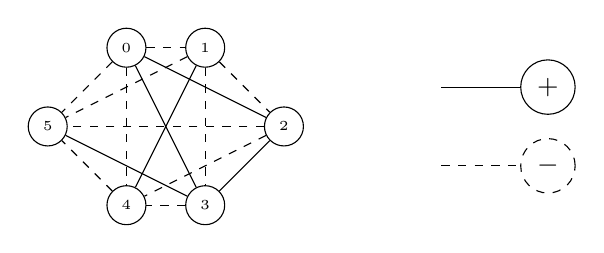
\begin{tikzpicture}
\node[draw, circle] at (0, 0) (a) {\tiny $0$};
\node[draw, circle] at (1, 0) (b) {\tiny $1$};
\node[draw, circle] at (2, -1) (c) {\tiny $2$};
\node[draw, circle] at (1, -2) (d) {\tiny $3$};
\node[draw, circle] at (0, -2) (e) {\tiny $4$};
\node[draw, circle] at (-1, -1) (f) {\tiny $5$};
%\draw (a) -- (0.5, -1) node[anchor=east] {\tiny $+$} -- (d);
%\draw (c) -- (1.5, -1.5) node[anchor=east] {\tiny $+$} -- (d);
%\draw (f) -- (0, -0.5) node {\tiny $+$} -- (b);
%\draw (b) -- (0.5, -1) node {\tiny $+$} -- (e);
\draw[dashed] (a) -- (b);
\draw[] (a) -- (c);
\draw[] (a) -- (d);
\draw[dashed] (a) -- (e);
\draw[dashed] (a) -- (f);
\draw[dashed] (b) -- (c);
\draw[dashed] (b) -- (d);
\draw[] (b) -- (e);
\draw[dashed] (b) -- (f);
\draw[] (c) -- (d);
\draw[dashed] (c) -- (e);
\draw[dashed] (c) -- (f);
\draw[dashed] (d) -- (e);
\draw[] (d) -- (f);
\draw[dashed] (e) -- (f);
\draw (4, -0.5) -- (5, -0.5) node[anchor = west] {$+$};
\draw[dashed] (4, -1.5) -- (5, -1.5) node[anchor = west] {$-$};
\end{tikzpicture}
\end{center}

    \subsubsection*{Solution}
    \begin{itemize}
        \item Ce graphe satisfait la propriété d'équilibre structurel.
        On peut séparer les noeuds en deux groupes : (0, 2, 3) et (1, 4, 5).
        Ces groupes ne contiennent que des liens positifs, et ne sont liés que par des liens négatifs.
        \item Ce graphe ne satisfait pas la propriété d'équilibre.
        Il contient des triangles faiblement équilibrés : (0, 4, 5), (1, 2, 3), (2, 3, 4), ...
        En revanche, il satisfait la propriété d'équilibre faible.
        On peut le séparer en 3 groupes : (0, 2), (1, 4) et (3, 5).
        \item Ce graphe ne satisfait pas la propriété d'équilibre.
        Il contient un triangle non-équilibré : (0, 3, 5).
    \end{itemize}
    

\subsection*{Exercice 9}
On prends un groupe de $n$ personnes et on ajoute des liens entre chaque paire de personnes avec le signe du lien choisi aléatoirement. Chaque lien est positif avec probabilit\'{e} $\frac{1}{2}$.
Quel est la probabilit\'{e} que le graphe soit structurellement \'{e}quilibr\'{e}? 
%Pour quels valeurs de $n$ est-ce que cette probabilit\'{e} est plus grande que $\frac{1}{2}$?

    \subsubsection*{Solution}
    On cherche le rapport du nombre de cas favorables sur le nombre de cas total.\\
    Puisque chaque arête prend 1 valeur parmi 2, et que le graphe est complet, il y a $2^{|E|} = 2^{\frac{n(n-1)}{2}} = 2^{\frac{n^2-n}{2}}$ cas possibles.\\
    On a $\frac{2^n}{2}$ cas favorables. \textbf{TODO : RAISONNEMENT}\\
    On a donc une probabilité de :
    $$ \dfrac{\dfrac{2^n}{2}}{2^{\frac{n^2-n}{2}}} = \dfrac{1}{2^{\frac{n^2-3n+2}{2}}}$$
    \noindent Cette probabilité vaut donc 0.5 dans le cas où $n=3$.
    Ce qui est logique, puisque dans ce cas on a 8 triangles possibles, dont 4 sont équilibrés.
    
    
    
\section{TP 11}
%\addcontentsline{toc}{section}{TP 11}

% \section*{Rappel}

% Structure du web:

% \begin{center}
% 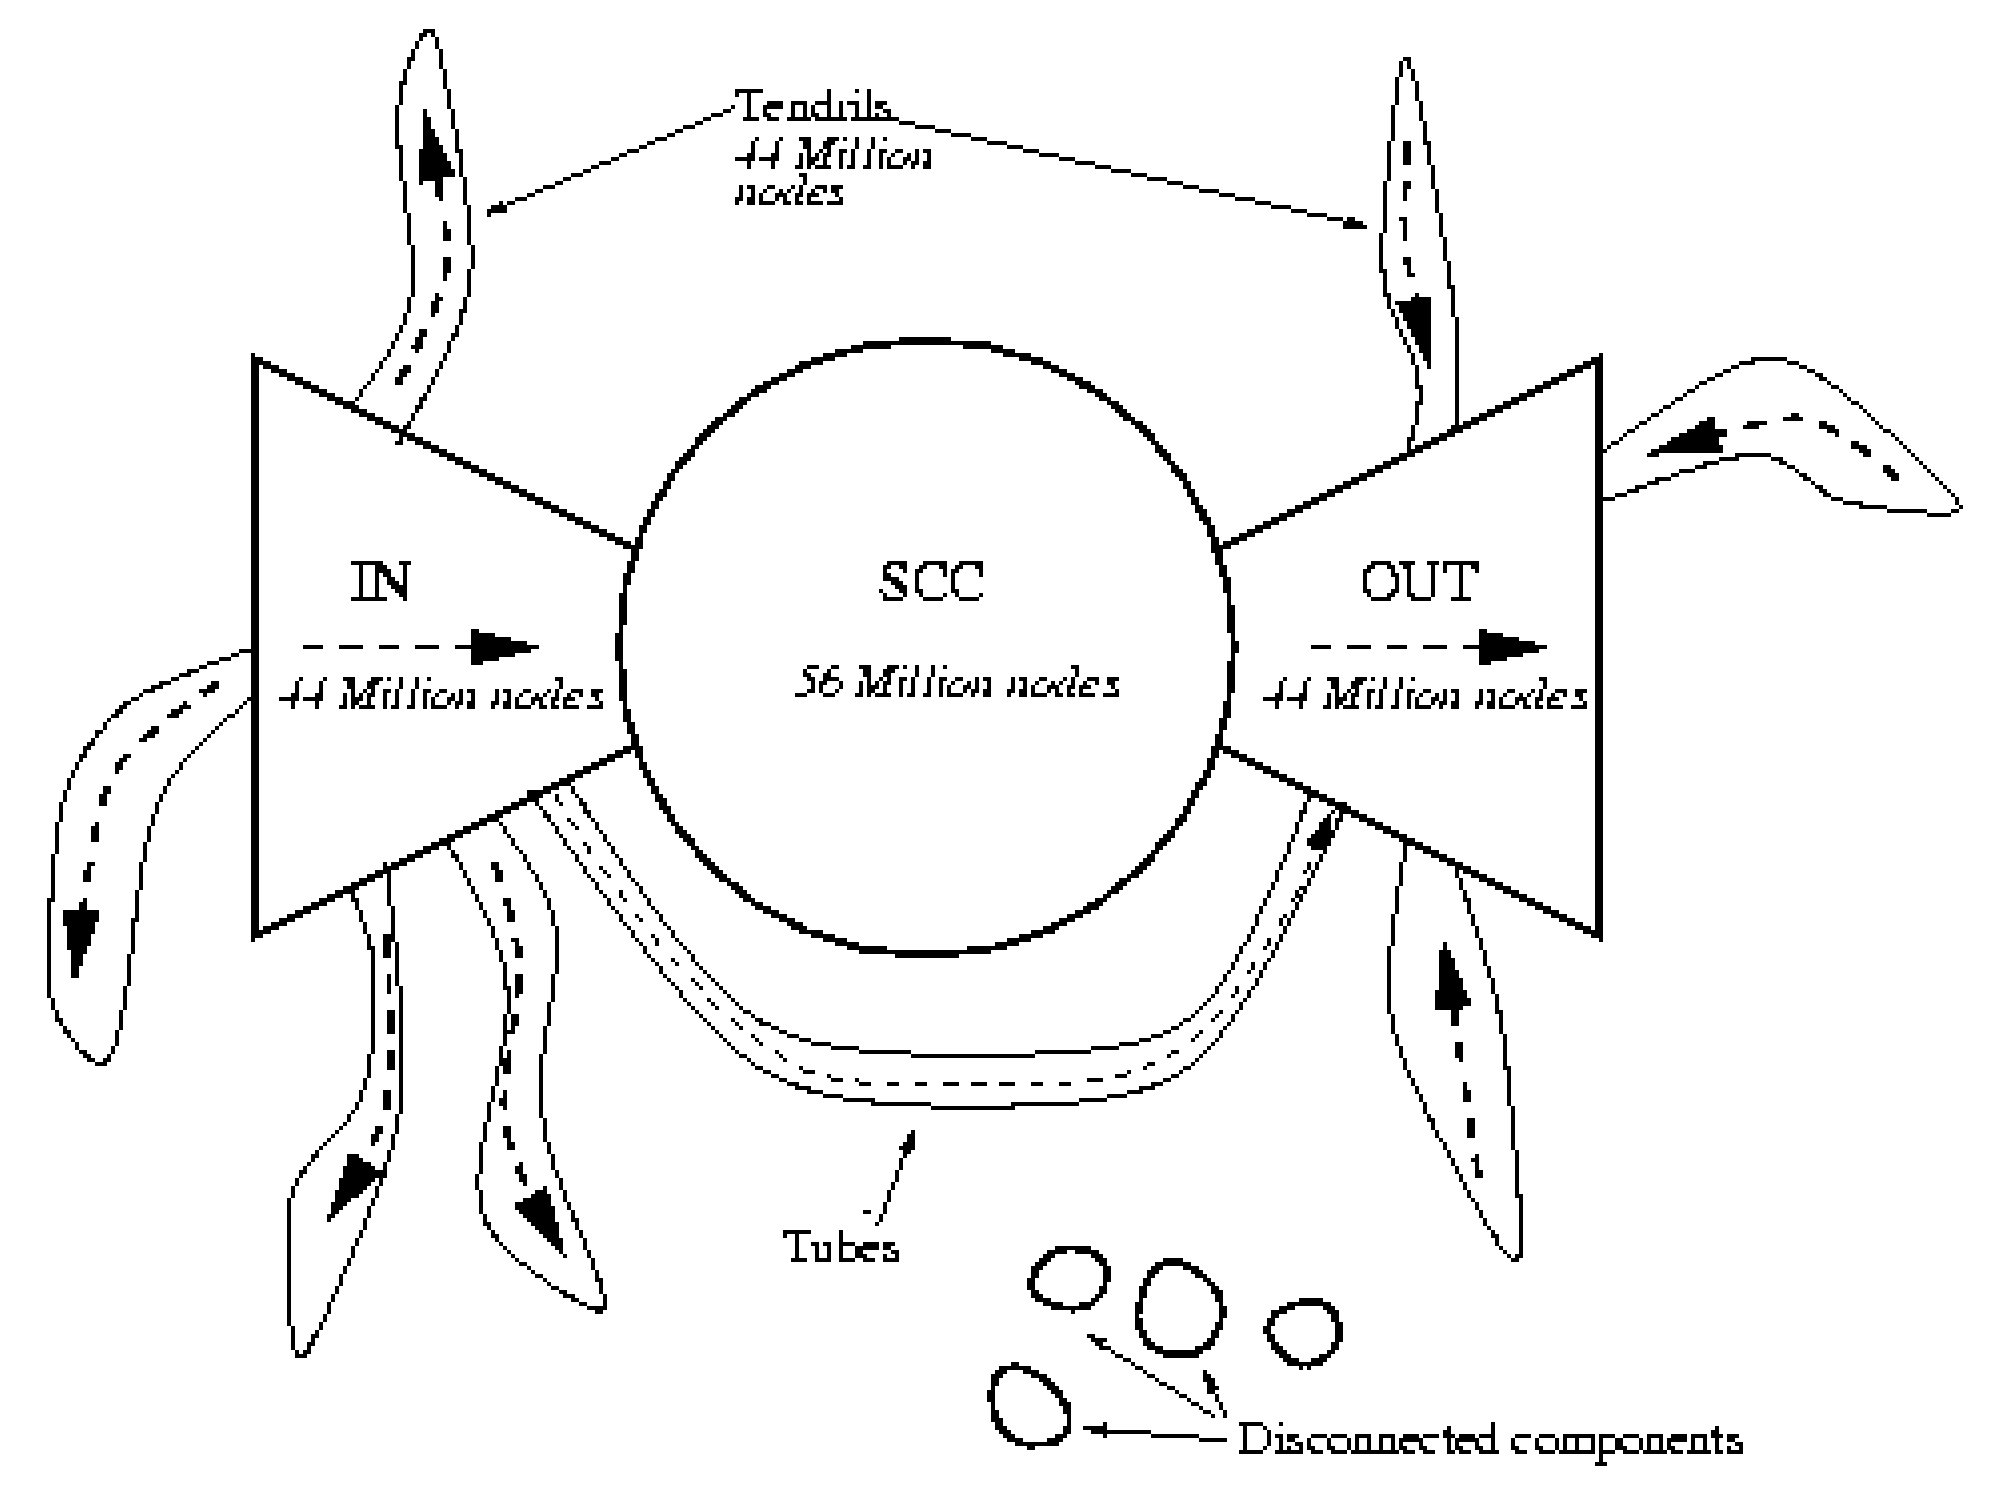
\includegraphics[scale = 0.5]{figs/web.png}
% \end{center}

% On repère trois composants principaux:
% \begin{itemize}
%  \item Un composant \textbf{in}, qui contient des liens hypertextes sortants.
%  \item Un composant fortement connecté principal, qui forme un \textbf{noyau} (SCC).
%  \item Un composant \textbf{out}, qui contient beaucoup de liens hypertextes entrants.
% \end{itemize}


% \newpage

% \section*{Exercices}


\subsection*{Exercice 1}
Considèrer de graphe avec 18 pages Web dans la Figure \ref{fig:webg}. Quels sont les noeuds qui font partie du noyau, les noeuds IN et les noeuds
OUT ?

    \begin{figure}[h!]
    \begin{center}
    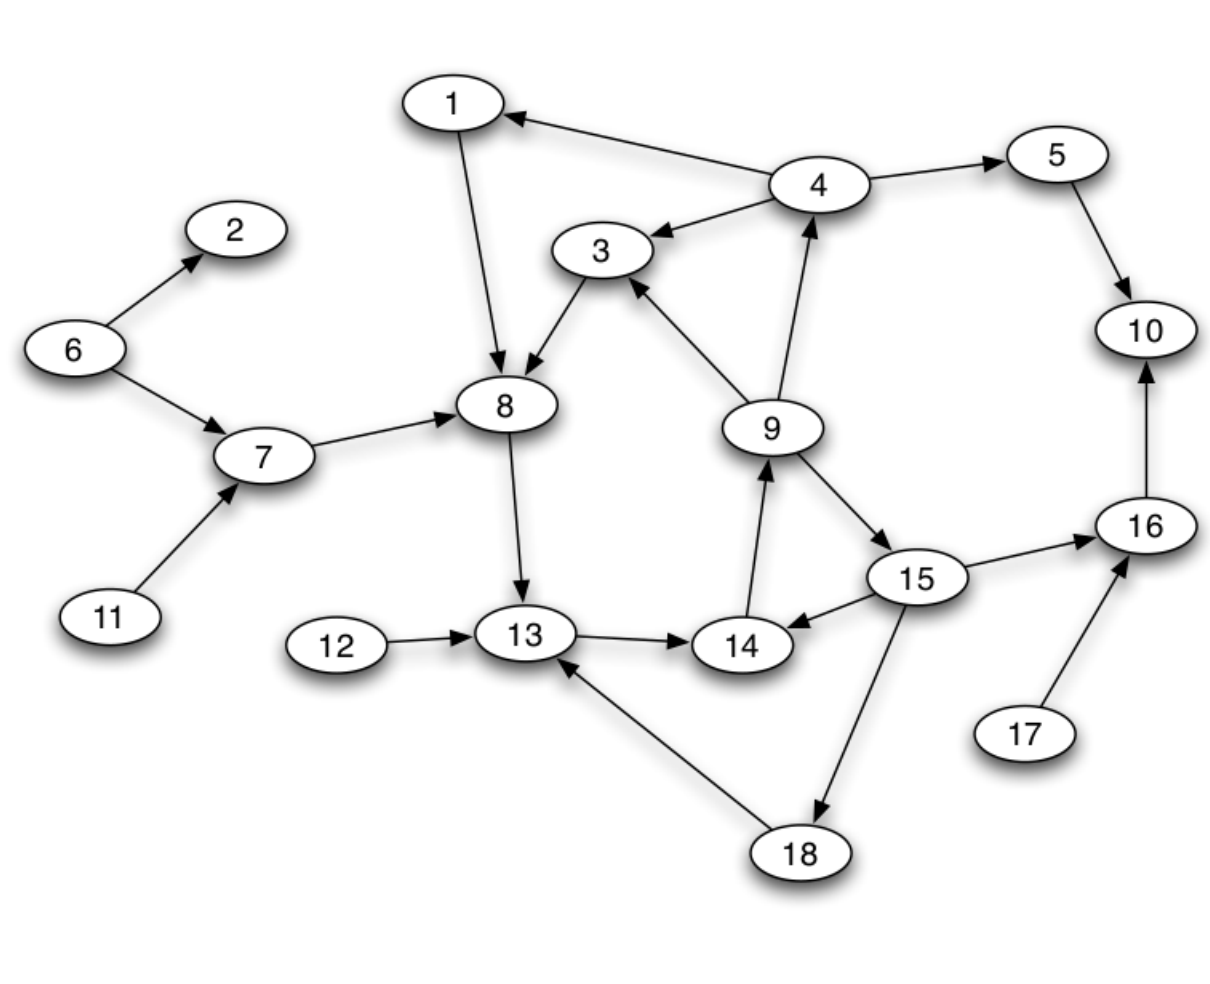
\includegraphics[scale = 0.3]{figs/graph.png}
    \end{center}
    \caption{Un graphe des pages web.}
    \label{fig:webg}
    \end{figure}

    \subsubsection*{Solution}

    \begin{center}
    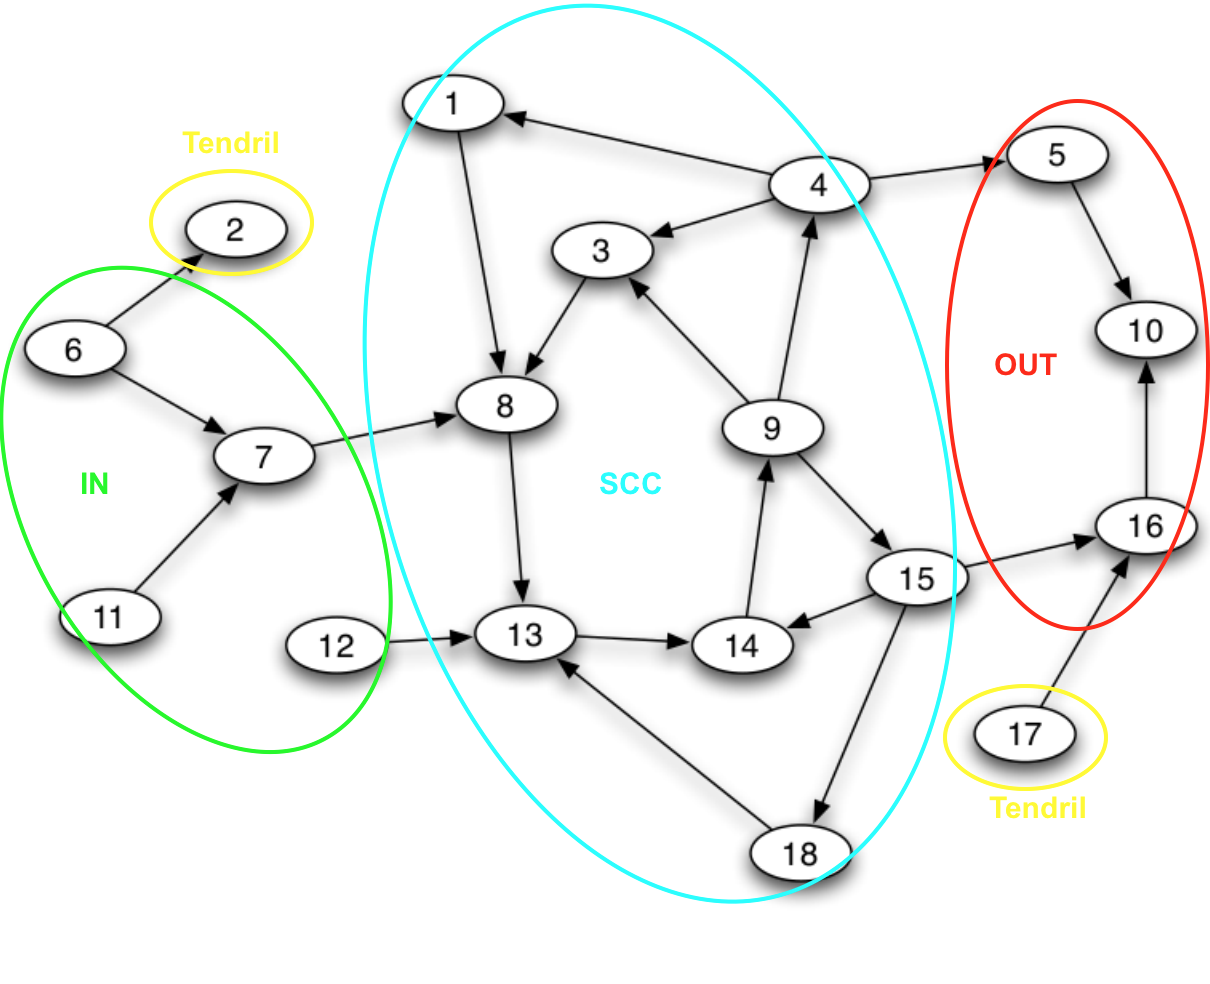
\includegraphics[scale=0.5]{figs/TP11Q1.png}
    \end{center}


\subsection*{Exercice 2}
Pour le graphe de la Figure \ref{fig:webg}.
\begin{enumerate}
 \item Montrez une arête tel que si on l'ajoute ou on la retire, on augmente la taille du noyau.
 \item Montrez une arête tel que si on l'ajoute ou on la retire, on augmente la taille de IN.
 \item Montrez une arête tel que si on l'ajoute ou on la retire, on augmente la taille de OUT.
\end{enumerate}

    \subsubsection*{Solution}

    \begin{center}
    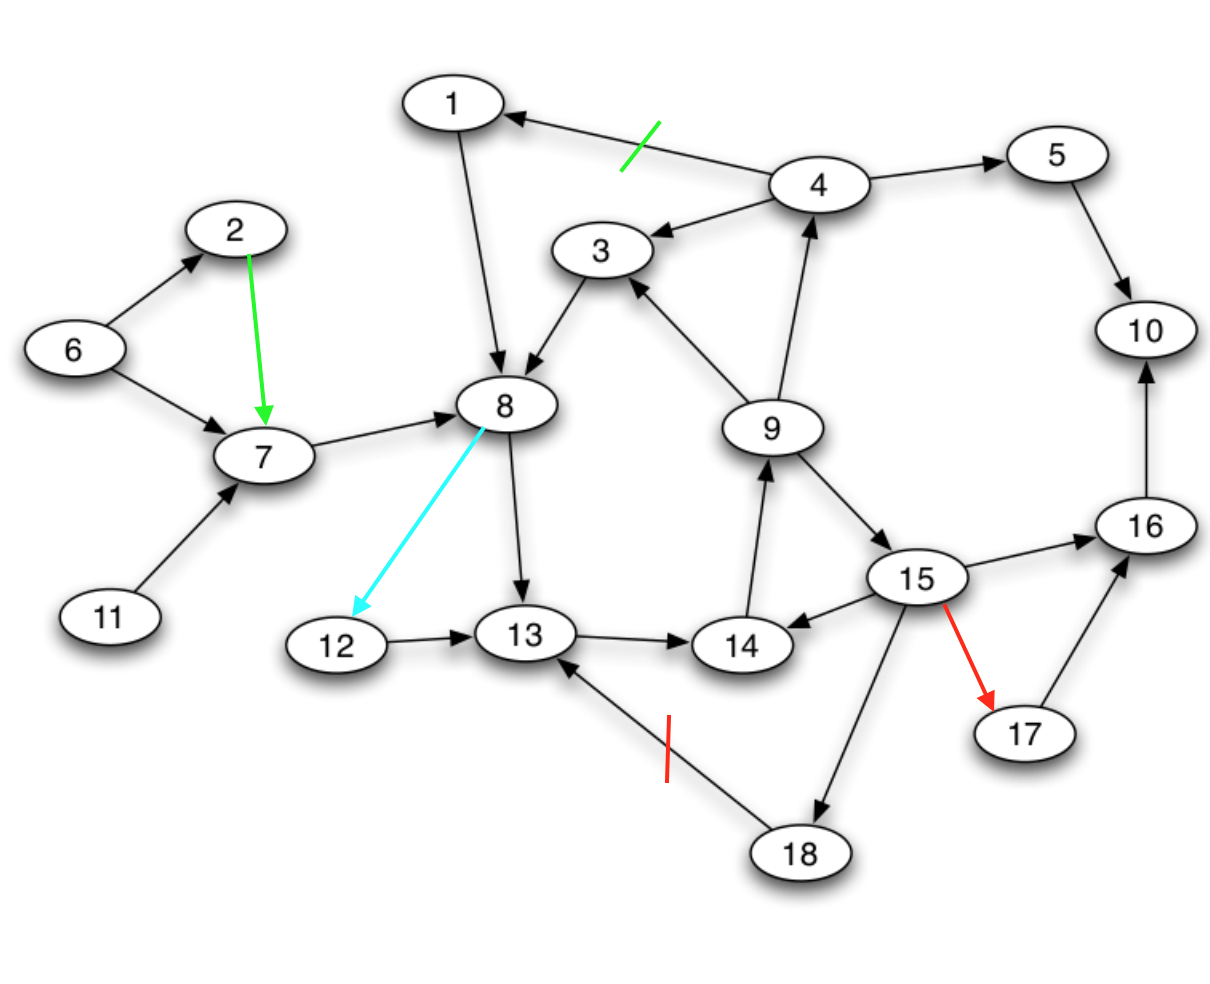
\includegraphics[scale=0.5]{figs/TP11Q2.png}
    \end{center}

    \begin{itemize}
        \item Le vert indique une arête à rajouter/retirer pour augmenter la taille du IN.
        \item Le rouge indique une arête à rajouter/retirer pour augmenter la taille du OUT.
        \item Le bleu indique une arête à rajouter pour augmenter la taille du SCC. Il n'est pas possible d'augmenter la taille du SCC en retirant une arête.
    \end{itemize}
    Il y a bien sûr d'autres possibilités que celles-là.


\subsection*{Exercice 3}
Décrivez un graphe tel qu'il existe une arête dont le retrait diminue la taille du noyeau d'au moins 1000 noeuds.

    \subsubsection*{Solution}
    Il faut pour cela un noyau qui possède un ensemble de 1000 noeuds ou plus qui n'est pas relié au IN ni au OUT et qui est relié au reste du noyau par seulement 2 arêtes : une entrante et une sortante.
    Supprimer l'arête qui va de cet ensemble au reste revient à rajouter l'ensemble au IN, tandis que supprimer l'autre arête revient à l'ajouter au OUT.


\subsection*{Exercice 4}
Décrivez un graphe tel qu'il existe une arête dont l'ajout diminue la taille de OUT d'au moins 1000 noueds.

    \subsubsection*{Solution}
    Il faut que le OUT possède une chaîne de 1000 noeuds ou plus et dont au moins un des noeuds de départ est directement lié au noyau.
    Il suffit de rajouter une arête au dernier noeud de cette chaîne pour qu'elle fasse partie intégrante du noyau, et donc pour diminuer la taille de OUT.

\subsection*{Exercice 5}
	\begin{enumerate}
	\item Calculez les valeurs de concentrateurs et d'autorités pour les pages dans le graphe présenté à la Figure \ref{fig:auth} après deux itérations.
	\item Quelles sont les valeurs une fois que la normalisation a été effectuée.
\end{enumerate}

\begin{figure}[!h]
	\centering
	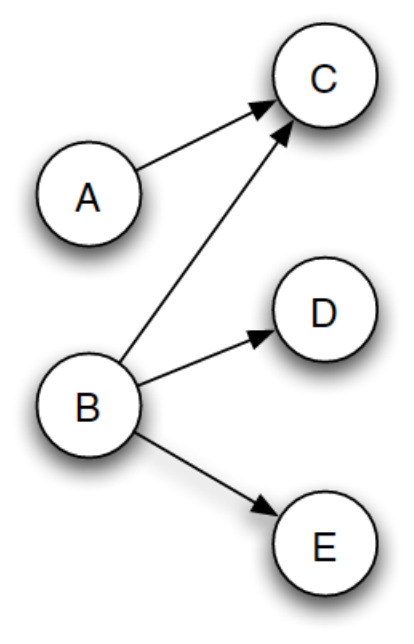
\includegraphics[scale=0.4]{figs/auth-hub.png}
	\caption{graphe de page web}
	\label{fig:auth}
\end{figure}

    \subsubsection*{Algorithme de normalisation}

    \begin{itemize}
        \item \textbf{Init} :  $ \forall x \: auth(x) = hub(x) = 1 $
        \item \textbf{Steps}: \\
            $\forall x \: auth(x) = \sum_{y \in hub(x)} hub(y)  $ \\
            $\forall x \: hub(x) = \sum_{y \in auth(x)} auth(y)  $
        \item \textbf{Normalisation} : \\
            $ \forall x \: auth(x) = \frac{auth(x)}{\sum auth} $ \\
            $ \forall x \: hub(x) = \frac{hub(x)}{\sum hub} $
    \end{itemize}

    \subsubsection*{Solution}
    \begin{itemize}
        \item \textbf{Auth} : authorité : liens entrants
        \item \textbf{Conc} : concentrateur : liens sortants
    \end{itemize}

    \begin{center}
    	\begin{tabular}{c|ccccc}
    	     & A & B & C & D & E\\ \hline
    	Auth & 1 & 1 & 1 & 1 & 1\\
    	Conc & 1 & 1 & 1 & 1 & 1\\ \hline
    	Auth & 0 & 0 & 2 & 1 & 1\\
    	Conc & 1 & 3 & 0 & 0 & 0\\ \hline
    	Auth & 0 & 0 & 4 & 3 & 3\\
    	Conc & 2 & 4 & 0 & 0 & 0\\ \hline
    	\end{tabular}
    \end{center}

    Normalisation :
    \begin{center}
    	\begin{tabular}{c|ccccc}
    	     & A & B & C & D & E\\ \hline
    	Auth & 0 & 0 & 0.4 & 0.3 & 0.3\\
    	Conc & $\frac{1}{3}$ & $\frac{2}{3}$ & 0 & 0 & 0\\ \hline
    	\end{tabular}
    \end{center}


\subsection*{Exercice 6}
Calculez les valeurs de PageRank pour chaque page dans le graphe présenté à la Figure \ref{fig:pagerank} après deux itérations avec S = 1.


\begin{figure}[ht!]
	\centering
	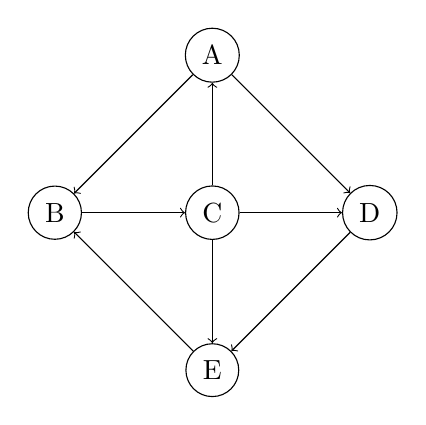
\begin{tikzpicture}[node distance=2cm]
		\tikzstyle{every node}=[draw=black,shape=circle]
		\node (c) at (0,0){C};
		\node[above of=c](a){A};
		\node[below of=c](e){E};
		\node[right of=c](d){D};
		\node[left of=c](b){B};

		\draw[->](a) -- (b);
		\draw[->](a) -- (d);
		\draw[->](b) -- (c);
		\draw[->](c) -- (a);
		\draw[->](c) -- (d);
		\draw[->](c) -- (e);
		\draw[->](d) -- (e);
		%\draw[->](d) -- (c);
		\draw[->](e) -- (b);
	\end{tikzpicture}
	\caption{graphe de page web}
	\label{fig:pagerank}
\end{figure}

    \subsubsection*{Solution}
    Règle de mise à jour : $Pr'(p) = S\ Pr(p) + (1-S) \frac{1}{n} = Pr(p)$.
    Seule la probabilité de suivre un lien à partir d'une page web entre en compte ici.\\
    À chaque itération k, on effectue les mises à jour suivantes :
    \begin{description}
        \item $Pr(A) = \frac{1}{3} Pr(C)$
        \item $Pr(B) = \frac{1}{2} Pr(A) + Pr(E)$
        \item $Pr(C) = Pr(B)$
        \item $Pr(D) = \frac{1}{2} Pr(A) + \frac{1}{3} Pr(C)$
        \item $Pr(E) = \frac{1}{3} Pr(C) + Pr(D)$
    \end{description}

    \begin{center}
        \begin{tabular}{c|ccccc}
        k & A & B & C & D & E\\ \hline
    	0 & $\frac{1}{5}$ & $\frac{1}{5}$ & $\frac{1}{5}$ & $\frac{1}{5}$ & $\frac{1}{5}$\\ \\
    	1 & $\frac{1}{15}$ & $\frac{3}{10}$ & $\frac{1}{5}$ & $\frac{1}{6}$ & $\frac{4}{15}$\\ \\
    	2 & $\frac{1}{15}$ & $\frac{3}{10}$ & $\frac{3}{10}$ & $\frac{1}{10}$ & $\frac{7}{30}$\\
    	\end{tabular}
    \end{center}

\subsection*{Exercice 7}
Dans la Figure \ref{fig:equi}, les nombres à coté des noeuds représentent la valeur de PageRank de la page. Avec ce graphe, les valeurs de PageRank forment-elles un ensemble équilibré? Si oui pourquoi? Si non pourquoi?

\begin{figure}[ht!]
	\centering
	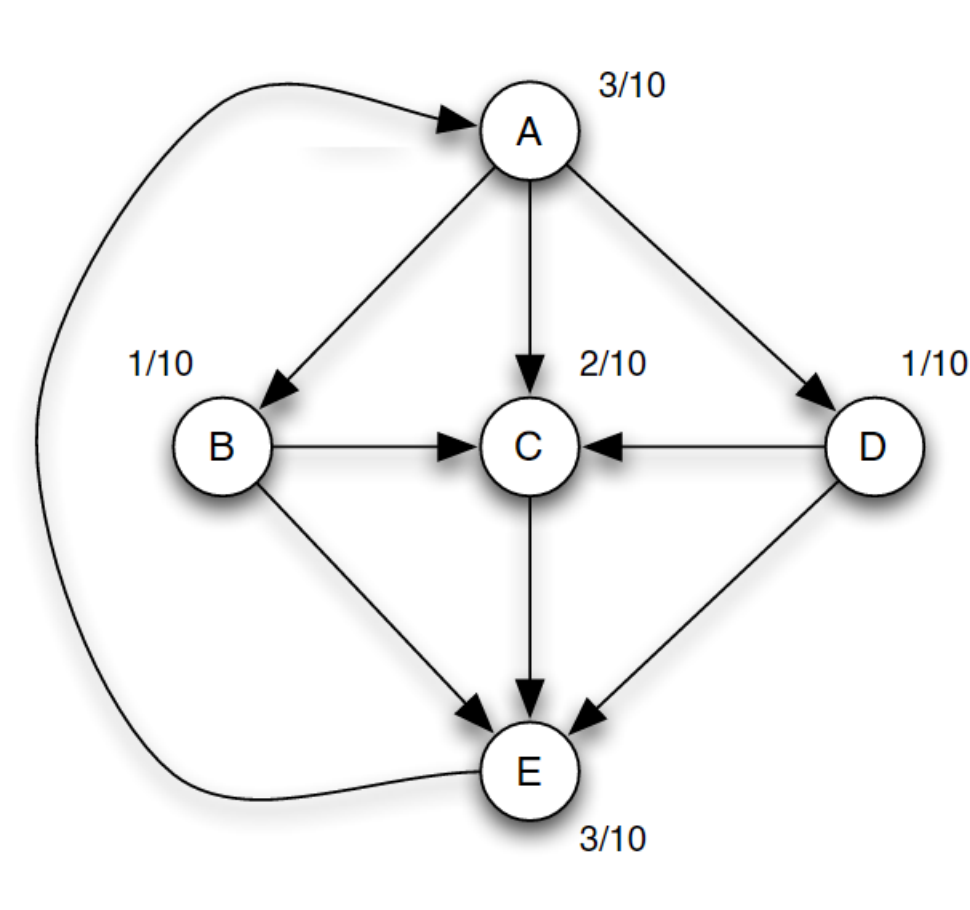
\includegraphics[scale=0.3]{figs/equi.png}
	\caption{graphe de page web}
	\label{fig:equi}
\end{figure}

    \subsubsection*{Solution}
    Il y a deux conditions à respecter pour que les valeurs de PageRank d'un graphe forment un ensemble équilibré :
    \begin{enumerate}
        \item La somme des valeurs doit valoir 1 : $\sum Pr(p_i) = 1$
        \item Une nouvelle itération doit donner les mêmes valeurs : $Pr'(p_i) = Pr(p_i) \ \forall p_i$\\
    \end{enumerate}

    Vérifions tout d'abord la première condition :
    $$ \sum Pr(p_i) = \frac{3}{10} + \frac{1}{10} + \frac{2}{10}  + \frac{1}{10}+  \frac{3}{10} = \frac{10}{10} = 1 $$

    Ensuite la seconde :
    \begin{description}
        \item $Pr'(A) = Pr(E) = \frac{3}{10} = Pr(A)$
        \item $Pr'(B) = \frac{1}{3} Pr(A) = \frac{1}{10} = Pr(B)$
        \item $Pr'(C) = \frac{1}{3} Pr(A) + \frac{1}{2} Pr(B) + \frac{1}{2} Pr(D) = \frac{2}{10} = Pr(C)$
        \item $Pr'(D) = \frac{1}{3} Pr(A) = \frac{1}{10} = Pr(D)$
        \item $Pr'(E) = \frac{1}{2} Pr(B) + Pr(C) + \frac{1}{2} Pr(D) = \frac{3}{10} = Pr(E)$\\
    \end{description}

    Nous pouvons donc conclure que nous cet ensemble de valeurs PageRank forme bien un ensemble équilibré.


\subsection*{Exercice 8}
		\begin{enumerate}
				\item Calculez les valeurs de PageRank pour chaque page dans le graphe présenté à la Figure \ref{fig:blackhole} après trois itérations avec S = 1.
				\item Que remarquez-vous? Selon vous comment vont évoluer les valeurs
						de PageRank pour un nombre d'itérations de plus en plus grand
				\item Calculez à nouveau les valeurs de PageRank pour chaque page mais pour 2 itérations avec S = 0.5.
		\end{enumerate}

    \begin{figure}[ht!]
	\centering

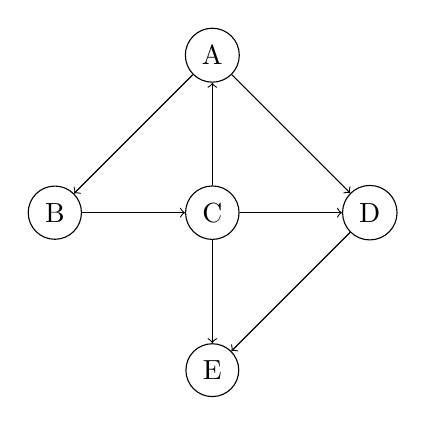
\begin{tikzpicture}[node distance=2cm]
	\tikzstyle{every node}=[draw=black,shape=circle]
	\node (c) at (0,0){C};
	\node[above of=c](a){A};
	\node[below of=c](e){E};
	\node[right of=c](d){D};
	\node[left of=c](b){B};

	\draw[->](a) -- (b);
	\draw[->](a) -- (d);
	\draw[->](b) -- (c);
	\draw[->](c) -- (a);
	\draw[->](c) -- (d);
	\draw[->](c) -- (e);
	\draw[->](d) -- (e);
	%\draw[->](d) -- (c);
	%\draw[->](e) -- (b);
\end{tikzpicture}
\caption{graphe de page web}
\label{fig:blackhole}
\end{figure}

    \subsubsection*{Solution}
    \begin{enumerate}

    \item Pour S=1, à chaque itération k, on effectue les mises à jour suivantes :
    \begin{description}
        \item $Pr(A) = \frac{1}{3} Pr(C)$
        \item $Pr(B) = \frac{1}{2} Pr(A)$
        \item $Pr(C) = Pr(B)$
        \item $Pr(D) = \frac{1}{2} Pr(A) + \frac{1}{3} Pr(C)$
        \item $Pr(E) = \frac{1}{3} Pr(C) + Pr(D) + Pr(E)$ \\
        \textit{(On ajoute $Pr(E)$ au calcul de E car c'est un noeud "cul-de-sac". Lors d'une itération, il faut prendre en compte le fait qu'une transition est bloquée au niveau de E et retombera donc vers E.)}
    \end{description}

    On obtient le résultat qui suit :
    \begin{center}
        \begin{tabular}{c|ccccc}
        k & A & B & C & D & E\\ \hline
    	0 & $\frac{6}{30}$ & $\frac{6}{30}$ & $\frac{6}{30}$ & $\frac{6}{30}$ & $\frac{6}{30}$\\ \\
    	1 & $\frac{2}{30}$ & $\frac{3}{30}$ & $\frac{6}{30}$ & $\frac{5}{30}$ & $\frac{14}{30}$\\ \\
    	2 & $\frac{2}{30}$ & $\frac{1}{30}$ & $\frac{3}{30}$ & $\frac{3}{30}$ & $\frac{21}{30}$\\ \\
    	3 & $\frac{1}{30}$ & $\frac{1}{30}$ & $\frac{1}{30}$ & $\frac{2}{30}$ & $\frac{25}{30}$\\
    	\end{tabular}
    \end{center}

    \item On remarque qu'il y a une accumulation au niveau du noeud E.
    Sa valeur va tendre vers 1 alors que toutes les autres tendent vers 0.

    \item Pour S=0.5, à chaque itération k, on effectue les mises à jour suivantes :
    \begin{description}
        \item $Pr'(A) = \frac{1}{6} Pr(C) + \frac{1}{10}$
        \item $Pr'(B) = \frac{1}{4} Pr(A) + \frac{1}{10}$
        \item $Pr'(C) = \frac{1}{2} Pr(B) + \frac{1}{10}$
        \item $Pr'(D) = \frac{1}{4} Pr(A) + \frac{1}{6} Pr(C) + \frac{1}{10}$
        \item $Pr'(E) = \frac{1}{6} Pr(C) + \frac{1}{2} Pr(D) + \frac{1}{2} Pr(E) + \frac{1}{10}$
    \end{description}

    Le tableau résultant est :
    \begin{center}
        \begin{tabular}{c|ccccc}
        k & A & B & C & D & E\\ \hline
    	0 & $\frac{6}{30}$ & $\frac{6}{30}$ & $\frac{6}{30}$ & $\frac{6}{30}$ & $\frac{6}{30}$\\ \\
    	1 & $\frac{4}{30}$ & $\frac{4.5}{30}$ & $\frac{6}{30}$ & $\frac{5.5}{30}$ & $\frac{10}{30}$\\ \\
    	2 & $\frac{4}{30}$ & $\frac{4}{30}$ & $\frac{5.25}{30}$ & $\frac{5}{30}$ & $\frac{11.75}{30}$\\
    	\end{tabular}
    \end{center}


\end{enumerate}


\end{document}
